\documentclass[a4paper,12pt, oneside]{book}

% \usepackage{fullpage}
\usepackage[italian]{babel}
\usepackage[utf8]{inputenc}
\usepackage{amssymb}
\usepackage{amsthm}
\usepackage{graphics}
\usepackage{amsfonts}
\usepackage{listings}
\usepackage{amsmath}
\usepackage{amstext}
\usepackage{engrec}
\usepackage{rotating}
\usepackage{verbatim}
\usepackage[safe,extra]{tipa}
%\usepackage{showkeys}
\usepackage{multirow}
\usepackage{hyperref}
\usepackage{microtype}
\usepackage{fontspec}
\usepackage{enumerate}
\usepackage{physics}
\usepackage{braket}
\usepackage{marginnote}
\usepackage{pgfplots}
\usepackage{cancel}
\usepackage{polynom}
\usepackage{booktabs}
\usepackage{enumitem}
\usepackage{framed}
\usepackage{pdfpages}
\usepackage{pgfplots}
\usepackage{algorithm}
% \usepackage{algpseudocode}
\usepackage[cache=false]{minted}
\usepackage{mathtools}
\usepackage[noend]{algpseudocode}

\usepackage{tikz}\usetikzlibrary{er}\tikzset{multi  attribute /.style={attribute
    ,double  distance =1.5pt}}\tikzset{derived  attribute /.style={attribute
    ,dashed}}\tikzset{total /.style={double  distance =1.5pt}}\tikzset{every
  entity /.style={draw=orange , fill=orange!20}}\tikzset{every  attribute
  /.style={draw=MediumPurple1, fill=MediumPurple1!20}}\tikzset{every
  relationship /.style={draw=Chartreuse2,
    fill=Chartreuse2!20}}\newcommand{\key}[1]{\underline{#1}}
  \usetikzlibrary{arrows.meta}
  \usetikzlibrary{decorations.markings}
  \usetikzlibrary{arrows,shapes,backgrounds,petri}
\tikzset{
  place/.style={
        circle,
        thick,
        draw=black,
        minimum size=6mm,
    },
  transition/.style={
    rectangle,
    thick,
    fill=black,
    minimum width=8mm,
    inner ysep=2pt
  },
  transitionv/.style={
    rectangle,
    thick,
    fill=black,
    minimum height=8mm,
    inner xsep=2pt
    }
  } 
\usetikzlibrary{automata,positioning,chains,fit,shapes}
\usepackage{fancyhdr}
\pagestyle{fancy}
\fancyhead[LE,RO]{\slshape \rightmark}
\fancyhead[LO,RE]{\slshape \leftmark}
\fancyfoot[C]{\thepage}
\usepackage[usenames,dvipsnames]{pstricks}
\usepackage{epsfig}
\usepackage{pst-grad} % For gradients
\usepackage{pst-plot} % For axes
\usepackage[space]{grffile} % For spaces in paths
\usepackage{etoolbox} % For spaces in paths
\makeatletter % For spaces in paths
\patchcmd\Gread@eps{\@inputcheck#1 }{\@inputcheck"#1"\relax}{}{}
\makeatother

\title{Teoria della Computazione}
\author{UniShare\\\\Davide Cozzi\\\href{https://t.me/dlcgold}{@dlcgold}}
\date{}

\pgfplotsset{compat=1.13}
\begin{document}
\maketitle

\definecolor{shadecolor}{gray}{0.80}
\setlist{leftmargin = 2cm}
\newtheorem{teorema}{Teorema}
\newtheorem{definizione}{Definizione}
\newtheorem{esempio}{Esempio}
\newtheorem{corollario}{Corollario}
\newtheorem{lemma}{Lemma}
\newtheorem{osservazione}{Osservazione}
\newtheorem{nota}{Nota}
\newtheorem{esercizio}{Esercizio}
\algdef{SE}[DOWHILE]{Do}{doWhile}{\algorithmicdo}[1]{\algorithmicwhile\ #1}
\tableofcontents
\renewcommand{\chaptermark}[1]{%
  \markboth{\chaptername
    \ \thechapter.\ #1}{}}
\renewcommand{\sectionmark}[1]{\markright{\thesection.\ #1}}
\newcommand{\floor}[1]{\lfloor #1 \rfloor}
\newcommand{\MYhref}[3][blue]{\href{#2}{\color{#1}{#3}}}%
\chapter{Introduzione}
\textbf{Questi appunti sono presi a lezione. Per quanto sia stata fatta
  una revisione è altamente probabile (praticamente certo) che possano
  contenere errori, sia di stampa che di vero e proprio contenuto. Per
  eventuali proposte di correzione effettuare una pull request. Link: }
\url{https://github.com/dlcgold/Appunti}.\\
\chapter{Prerequisiti di computazione}
L'informatica è costruita su una logica matematica. Il punto di partenza è stato
dettato da Turing (con la \textbf{macchina di Turing} (\textit{TM})) e questo
pensiero si è poi sviluppato nel tempo. Turing, con la sua macchina logica, ha
dimostrato che ci sono funzioni non calcolabili, verità logiche non
dimostrabili.\\ Subito dopo la macchina di Turing nasce la teoria della
\textbf{complessità   computazionale}, col fine di classificare il problemi in
base alla difficoltà delle soluzioni mediante macchine di calcolo. Tale
\textit{difficoltà} viene stimata rispetto a \textbf{spazio e tempo}. La teoria
della \textbf{complessità computazionale} si riferisce a varie \textbf{classi
  di complessità} che 
classificano, in un primo approccio, \textit{problemi decisionali} descritti da
funzioni binarie che hanno in input una stringa sull'alfabeto $\{0,1\}$ e
restituiscono un bit (o 0 o 1). Questo perché le macchine di Turing ragionano in
binario. Si ha quindi:
\[f:\{0,1\}^*\to {0,1}\]
\textbf{Esistono problemi che si è dimostrato non essere risolvibili in tempo
  efficiente.}\\
Tra le classi abbiamo i \textbf{problemi NP} e \textbf{problemi P}. Inoltre i
problemi NP sono a loro volta classificabili tra loro cercando i più difficili,
ottenendo \textbf{problemi NP-hard} e \textbf{problemi NP-complete} (esistono
varie dimostrazioni per la \textit{NP-completezza}).
\section{Tempo di calcolo di una TM}
\begin{definizione}
  Sia $T:\mathbb{N}\to \mathbb{N}$ una funzione calcolabile da TM e $L\pi$ un
  linguaggio di decisione (dove $\pi$ sta per ``problema'' e ``di decisione'' ci
  ricorda che il risultato sarà binario) allora una \textbf{TM deterministica}
  $M$ accetta L$\pi$ in tempo $T(n)$ se, $\forall x\in L\pi$, con $|x|=n$, $M$
  accetta $x$ in $T(n)$ mosse o configurazioni
\end{definizione}
\begin{definizione}
  Un \textbf{problema di decisione} $\pi$ riceve in input un'istanza $x$ e
  l'output è:
  \begin{itemize}
    \item 0 che vuole dire \textit{no}
    \item 1 che vuole dire \textit{yes}
  \end{itemize}
  Un linguaggio $L\pi$ restituisce 1 per tutti gli $x$ che appartengono al
  linguaggio. Quindi $L\pi$ è l'insieme degli input di $\pi$ su cui l'output è
  1 (è l'analogo della \emph{funzione caratteristica} di un insieme, ovvero la
  funzione che risponde 1 sse un certo elemento appartiene all'insieme di
  riferimento).\\
  La \textbf{funzione associata al problema} si chiama $f\pi$ ed è la funzione
  che dato un input restituisce 1 sse l'input appartiene al $L\pi$.
\end{definizione}
Approfondiamo ora lo studio della \textbf{classe P}.
\begin{definizione}
  La classe dei linguaggi di decisione accettati in tempo
  $T(n)=cn^p,\,p\in\mathbb{N},\, p\neq 0$ da una TM deterministica è detta
  \textbf{classe P}, quindi in un tempo polinomiale sulla dimensione dell'input
  $n$, è detta \textbf{classe P}. Quindi P è una classe di \textbf{problemi di
    decisione}. \\
  Potenzialmente $p$ potrebbe anche non essere un intero in quanto si potrebbero
  avere tempi frazionari.
\end{definizione}
\begin{definizione}
  Si definisce che $L\pi$ è accettato da una TM in tempo $T(n)$ se $\exists
  \,\,T :\mathbb{N}\to \mathbb{N}$ calcolabile da TM e $\forall x\in L\pi$, con
  $|x|=n$, la TM accetta $x$ e risponde 1 (\textit{yes}) in al più $T(n)$ mosse
  di calcolo (dette anche configurazioni).\\
  Nel caso del modello della macchina RAM si ha la stessa situazione con però
  $T(n)$ \textbf{istruzioni RAM} e si dice che $L\pi$ è accettato dalla macchina
  RAM (si può dire che è anche deciso dell'algoritmo A della macchina RAM). In
  caso contrario la macchina RAM restituisce \textit{no}, in quanto si parla di
  ``decisione'' oltre che di ``accettazione'' (a differenza della TM, dove però
  si può ottenere lo stesso discorso parlando di TM complementare $M'$, che in
  $T(n)$ mi risponderà yes alla richiesta che un input non appartenga a
  $L\pi$, altrimenti bisogna fissare un limite di tempo per ottenere yes).\\
  È dimostrabile che se $L\pi$ è accettabile in tempo polinomiale allora nello
  stesso tempo è anche decidibile.\\
  La differenza tra accettazione e decisione sarà fondamentale nel
  \textbf{modello non deterministico}.
\end{definizione}
\begin{shaded}
  Si ricordi che il \textbf{modello RAM (\textit{Random Access Machine})} è
  usato per studiare il tempo di calcolo di 
  uno pseudocodice. È un modello teorico (una macchina teorica ``simile'' a
  quelle reali) dotato di istruzioni come
  \textit{load, store, add, etc$\ldots$} dove un codice (ipoteticamente in
  qualsiasi linguaggio incluso lo pseudocodice) viene tradotto in una sorta di
  linguaggio macchina (linguaggio RAM), dove $n$ è un intero rappresentante il
  numero di istruzioni RAM necessarie per ottenere l'output ($n$ è detto
  \textbf{tempo uniforme}). Sul linguaggio RAM si può studiare anche lo spazio
  calcolato come numero di bit necessari per la computazione (è detto
  \textbf{costo logaritmico}). In questo secondo punto il costo di
  un'istruzione, come ad esempio \textit{load(n)}, è logaritmico rispetto
  all'operando $n$ ($\,\log_2 n$), studia quindi la \emph{dimensione}
  dell'input.
\end{shaded}
Consideriamo ora un modello basato su algoritmi.
\begin{definizione}
  Sia $L\pi$ un linguaggio di decisione e $t:\mathbb{N}\to\mathbb{N}$ una
  funzione calcolabile, allora un algoritmo $A$ accetta $L\pi$ in tempo $T(n)$
  sse $\forall x\in L\pi$, con $|x|=n$, $A$ termina su input $x$ dopo $T(|x|)$
  passi di calcolo, ovvero istruzioni esguite, producendo 1 come output. Quindi
  P è la classe dei linguaggi di decisione accettati in tempo
  $T(n)=cn^p,\,p\in\mathbb{N}$ (con lo stesso discorso di sopra su $p$) da un
  algoritmo $A$ in tempo polinomiale.
\end{definizione}
\chapter{Complessità computazionale}
Si cerca di catalogare dal punto di vista computazionale i \textbf{problemi
  intrattabili}, ovvero problemi risolvibili ma non in modo \textbf{efficiente}
(ovvero in tempo polinomiale). In alcuni casi si pensa che non esista una
soluzione ma non si hanno dimostrazioni in merito mentre in altri casi è
addirittura dimostrato. Abbiamo quindi delle categorie informali per i problemi:
\begin{itemize}
  \item \textbf{facili}, so risolverli in modo efficiente. È la \textbf{classe P}
  \item \textbf{difficili} o, più formalmente, \textbf{intrattabile}, so
  risolverli ma non in modo efficiente e non ho una 
  dimostrazione che mi assicuri che non siano risolvibili in modo efficiente. È
  la \textbf{classe NP} e la sua sottoclasse \textbf{NP-complete}
  \item \textbf{dimostrabilmente difficili}, so risolverli ma so che non esiste
  un algoritmo efficiente in quanto è stato dimostrato che non può esistere
  \item \textbf{impossibili}, non so risolverli sempre neanche in modo non
  efficiente (esiste almeno un input che manda in crisi l'algoritmo ma esiste
  almeno un caso in cui funzioni)
\end{itemize}
Come formalismo useremo la \textbf{Macchina di Turing (\textit{TM})},
\textit{deterministica} e \textit{non deterministica}. Analizzeremo in primis
\textbf{problemi sui grafi}. Un grafo è definito come $G=(V,E)$, con $V$ insieme
dei vertici e $E$ insieme degli archi. Un grafo può essere \textit{orientato} o
\textit{non orientato}. Un \textbf{cammino} tra due vertici è una sequenza di
archi che mi porta da un vertice all'altro. Un cammino è detto \textbf{ciclo} se
il vertice sorgente coincide con quello di destinazione. Due vertici sono
\textbf{connessi} se esiste un cammino che li collega. Un \textbf{grafo
  connesso} è un grafo dove per ogni coppia di vertici si ha che essi sono
connessi. Se questo cammino è di un solo arco si parla di \textbf{grafo
  completo}, ovvero ogni vertice è \textbf{adiacente} ad ogni altro. Si parla di
\textbf{grafo pesato} se si ha una funzione $W$ che associa un peso ad ogni
arco. \\
Useremo anche la teoria dei linguaggi formali con $V$ alfabeto e stringhe
costruite su $V$. Con $\varepsilon$ abbiamo la stringa vuota e con $V^*$ è
l'insieme di tutte le possibili stringhe costruibili con quell'alfabeto, inclusa
la stringa vuota. $V^*$ è un insieme infinito. Con $V^+$ indico
$V^*/\varepsilon$, ovvero senza la stringa vuota. Un \textbf{linguaggio} $L$ è
un sottoinsieme di $V^*$, quindi $L\subseteq V^*$, che comprende tutti gli
elementi di $V^*$ che seguono una certa \textbf{proprietà} (o più
proprietà). Anche $L$ è un insieme infinito.\\
Un'altra nozione è quella di \textbf{problema}. Un problema computazionale è una
``questione'' a cui si cerca risposta. Più formalmente un problema è specificato
da \textbf{parametri} (l'input del problema) e le \textbf{proprietà} che deve
soddisfare la \textbf{soluzione} (l'output). L'\textbf{istanza} di un problema
specificando certi parametri in input al problema (input che devono essere
coerenti ai parametri richiesti).\\
Cominciamo con degli esempi di problemi comunque risolvibili.
\begin{esempio}
  Considero il problema \emph{arco minimo}. Come parametro ho un grafo pesato
  sugli archi $G=(V,E)$. Le proprietà della soluzione è che voglio l'arco con
  peso minimo.\\
  Per risolvere guardo tutti gli archi è vedo quello di peso minimo. Dato che
  basta iterare su tutti gli archi quindi la soluzione è in $O(n)$ (in realtà
  $\Theta(n)$), quindi in \textbf{tempo lineare} sul numero di archi (è quindi
  in \textbf{tempo polinomiale})
\end{esempio}
\begin{esempio}
  Considero il problema \emph{raggiungibilità}. Come parametro ho un grafo non
  pesato $G=(V,E)$ e due vertici, uno sorgente e uno destinazione, tali che
  $v_s,v_d\in V$. Le proprietà della soluzione è che voglio sapere se posso
  arrivare a $v_d$ partendo da $v_s$.\\
  Per risolvere studio tutti i cammini che partono da $v_s$ e posso dare la
  risposta. Una soluzione del genere è in tempo $O(2^{|E|})$. Il tempo quindi
  cresce in \textbf{modo esponenziale}. Una soluzione migliore è quella di usare
  un \textbf{algoritmo di visita} che richiede tempo $O(|V|+|E|)$, ovvero un
  \textbf{tempo polinomiale}. Quindi per quanto all'inizio si pensi
  che sia un \textbf{problema intrattabile} si scopre che è un \textbf{problema
    facile} 
\end{esempio}
\begin{esempio}
  Considero il problema \emph{TSP}. Come parametro ho un grafo pesato sugli
  archi e completo $G=(V,E)$. Le proprietà della soluzione è che voglio sapere
  il \emph{cammino minimo} (in realtà un ciclo) che tocca tutti i vertici una e
  una sola volta (una volta trovata la soluzione non mi interessa la sorgente
  essendo il grafo completo). \\
  Sarebbe facile determinare \textbf{un} ciclo ma non quello di peso minimo e
  per farlo devo trovare tutti i cicli e trovare quello di peso minimo. Ho
  quindi un algoritmo che è $O(2^n)$ (nella realtà è circa $O(n!)$ che è
  comunque esponenziale per l'\textbf{approssimazione di Stirling}). In questo
  caso non si riesce a pensare ad una soluzione che non sia esponenziale nel
  tempo (anche se per alcuni input sia di facile risoluzione, basti pensare ad
  avere tutti gli archi di peso 1, ma mi basta avere un input problematico). Non
  potendo però dimostrare che sia irrisolvibile si dice che è un
  \textbf{problema intrattabile}. \textit{TSP} è uno dei 10 problemi famosi per
  i quali ti danno un milione di dollari se dimostri che è o \emph{facile} o
  \emph{impossibile}
\end{esempio}
Per completezza definiamo un \textbf{algoritmo} come una sequenza di
\textbf{istruzioni elementari} (supportate dal calcolatore) che, eseguite in
sequenza, mi portano alla soluzione di un problema. Si ha quindi che un
algoritmo $A$ risolve un problema $\Pi$ se per ogni possibile istanza di $\Pi$
l'algoritmo $A$ mi da la risposta corretta. Distinguo però:
\begin{itemize}
  \item \textbf{algoritmo efficiente}, che mi da la soluzione in \textbf{tempo
    polinomiale} rispetto alla \textbf{dimensione dell'input}. Ho un
  \textit{caso peggiore} limitato superiormente da un \textbf{polinomiale}:
  $O(p(n))$. Ho una crescita di tempo accettabile all'aumentare
  dell'input. Diciamo comunque che è dura anche solo raggiungere $O(n^{10})$
  quindi anche se dire polinomiale potrebbe voler dire $O(n^{10000000})$ non si
  hanno casi reali di questo tipo
  \item \textbf{algoritmo non efficiente}, che mi da la soluzione ma in tempo
  superiore a quello \textbf{polinomiale}. Ho un \textit{caso peggiore} limitato
  superiormente da un \textbf{esponenziale}: $O(2^n)$. Ho una crescita di tempo
  assolutamente non accettabile (esponenziale appunto) all'aumentare dell'input 
\end{itemize}
\textit{Se ho anche solo un caso di input che porta a tempo esponenziale ho
  comunque un algoritmo non efficiente}.\\
Spesso \textbf{problemi intrattabili} vengono risolti tramite approssimazioni
per arrivare ad una soluzione accettabile anche se non la migliore ma non sempre
è possibile effettuare delle approssimazioni.\\
Anche se avessi ha che fare con un computer mille volte migliore di quelli
attuali, un problema esponenziale avrà comunque tempi non accettabili in
proporzione ad un problema polinomiale. Quindi non sarà il miglioramento
hardware a permettere di rendere accettabile la soluzione di problemi
esponenziali.\\
Un \textbf{algoritmo intrattabile} quindi non risolve in modo efficiente tutti
gli input. Bisognerà trovare un modo per capire se un algoritmo è
\textbf{intrattabile} per davvero.\\
Studiamo ora il tempo di calcolo di una \textbf{macchina di Turing non
  deterministica (\textit{NTDM})}:
\begin{definizione}
  Sia $T:\mathbb{N}\to\mathbb{N}$ una funziona calcolabile da TM. Dato $L\pi$ un
  linguaggio di decisione allora una $NDTM$ $M$. $M$ accetta $L\pi$ in tempo
  $T(n)$ se per ogni $x$ in $L\pi$ ,con $|x|=n$,  $M$ accetta $x$ in $T(n)$
  mosse (o configurazioni).\\
  Quindi la \textbf{classe NP} è la classe dei linguaggi di decisione accettati
  in tempo $T(n)=cn^p,\,\,\,p\in \mathbb{N}$ da una $NDTM$
\end{definizione}
Diamo una definizione alternativa di NP:
\begin{definizione}
  Sia $L\pi$ un linguaggio di decisione, $N:n\to n$ una funzione calcolabile,
  $y$ una stringa di lunghezza polinomiale nell'input, allora un algoritmo $A$
  con ``certificato'' accetta $L\pi$ in tempo $t(n)$ se per ogni $x$ in $L\pi$,
  con $|x|=n$, A termina su input $(x,y)$ dopo $t(|x|)$ passi di calcolo
  (istruzioni eseguite) producendo 1 in output.
  Quindi la \textbf{classe NP} è la classe dei linguaggi (o problemi) di
  decisione accettati in tempo $T(n)=cn^p,\,\,\,p\in\mathbb{N}$ da un algoritmo
  $A$ ``certificato''
\end{definizione}
Resta da capire il significato del termine ``certificato''.
\begin{definizione}
  Preso un algoritmo $A$ definiamo cosa significa che sia ``certificato'' si
  compone di un input $(x,y)$ con $y$ che è una stringa, nel dettaglio una
  \textbf{dimostrazione}, che garantisce che $x\in L\pi$.
\end{definizione}
Vediamo un esempio:
\begin{esempio}
  Uso un problema NP come esempio, quindi $\pi\in NP$, per avere un algoritmo
  che ammette certificato (non ho alternative). \\
  Prendo il problema $\pi$ \emph{vertex-cover}. Come input si ha un grafo
  $G=(V,E)$ e un intero $k$. Come output ho o 1 o 0, essendo un problema di
  decisione, e si cerca di capire se $\exists\, V'\subseteq V$ tale che $V'$ è
  una copertura di $G$. Il sottoinsieme è copertura di un grafo quando $forall\,
  e\in E$ almeno un estremo dell'arco $e=(u,v)$ è in $V'$. La copertura con il
  minor numero di vertici è detta \textbf{minima copertura}.\\
  Il problema \emph{vertex-cover} chiede se esiste una copertura del grafo di
  dimensione $k$. È quindi un \textbf{problema di decisione}. Qualora trovassi
  una copertura di cardinalità minore di $k$ mi basterà aggiungere vertici
  arbitrari fino al raggiungimento di $k$. Ovviamente può non esistere una
  copertura di cardinalità $k$.\\
  Il problema di \emph{vertex-cover} è il problema di decisione del problema di
  trovare la minima copertura di un grafo, che è un \textbf{problema di
    ottimizzazione (o problema di ottimo)} (ogni problema di ottimizzazione può
  essere trasformato in uno di decisione aggiungendo un parametro $k$ e
  richiedendo un risultato booleano).\\
  \emph{vertex-cover} decisionale è nella classe \textbf{NP} con ``certificato''
  e, in questo caso, il parametro $y$ è la dimostrazione che posso dare risposta
  affermativa, per esempio la certezza di avere un sottoinsieme di vertici che
  effettivamente copre tutto il grafo, quindi $y=V''\subseteq V$ tale per cui
  $V''$ copre $G$ con cardinalità $k$. Bisogna capire come trovare e come usare
  $y$, sapendo che $A$ lavora in tempo polinomiale e che la lunghezza di $y$ è
  polinomiale in dimensione di $x$.\\ 
  Vedendo che la cardinalità di $y$ è minore di $k$ l'algoritmo A verifica che
  con i vertici passati con $y$ si è in grado di rispondere al problema in modo
  affermativo, problema che ha in input $G$ e $k$. In poche parole $A$, per ogni
  arco, esamina se ogni estremo è in $y$ e, se tutti gli archi hanno un estremo
  in $y$ allora si ha che usando $y$ si è in grado di verificare l'input $G,
  k$ è \textbf{accettato}. Questa verifica è in tempo polinomiale e si ha che
  $|y|=O(|G,k|)$, soprattutto se $|y|$ è una costante.\\
  Ad oggi non si è dimostrato che \emph{vertex-cover} si risolvibile in tempo
  polinomiale. È quindi un problema \textbf{NP-hard}.
\end{esempio}
\begin{esempio}
  Per l'algoritmo TSP la versione di ottimo è trovare il \emph{tour} di costo
  minimo. Il problema di decisione è se esiste un \emph{tour} di massimo peso
  $k$. In questo caso già il problema di decisione è già in \textbf{NP} e lo è
  anche il problema di ottimo. La verifica con ``certificato'' ha comunque costo
  polinomiale nel caso di richiesta di verifica di un dato \emph{tour} con costo
  minore di $k$. 
\end{esempio}
\textbf{Il problema di decisione è una restrizione di quello di ottimo.}\\
Per notazione dato un algoritmo $A$ chiamiamo $A_d$ la sua versione di
decisione.\\

\textbf{Senza ``certificato'' non potrei accettare un problema NP}.\\
Un problema di \textbf{classe NP} quindi ammette verifica in tempo polinomiale,
ammettendo un ``verificatore'' in tempo polinomiale per i problemi
specificati.\\
Non è così scontato trovare ``certificato'', di dimensione polinomiale
nell'input, e trovare il ``verificatore''. Per esempio la classe
\textbf{exptime} non esiste $A$ con ``certificato'' che sia polinomiale (la
verifica potrebbe richiedere tempo esponenziale).\\
Quindi per un problema \textbf{NP} con ``certificato'' non posso trovare
soluzione in tempo polinomiale ma posso verificare una soluzione data in tempo
polinomiale.\\
Posso quindi dimostrare che un problema $\pi$, con in input una struttura
combinatoria discreta (come un grafo) e un intero, è in \textbf{NP}.\\
Si ha quindi che \textbf{P} è vista come sottoclasse la \textbf{NP} dove i
problemi di decisione sono risolvibili in tempo polinomiale anche senza
``certificato''. Per dimostrare che $P\subseteq NP$ devo far vedere che ogni
$L\pi\in P$ ammette un algoritmo $A$ con ``certificato'' in tempo
polinomiale. Ma questo è vero perché $L\pi$ è accettato da un algoritmo $A$, in
tempo polinomiale con $y=\emptyset$ e quindi $y$ non è necessario.\\
Si ha quindi che $P\subseteq NP$. Pensando poi, per esempio,
all'\textit{isomorfismo di grafi} nessuno sa se sia $P$ o $NP$. Questo
problema ha in input due grafi e come output se sono isomorfi tra loro.
\begin{figure}[H]
  \centering
  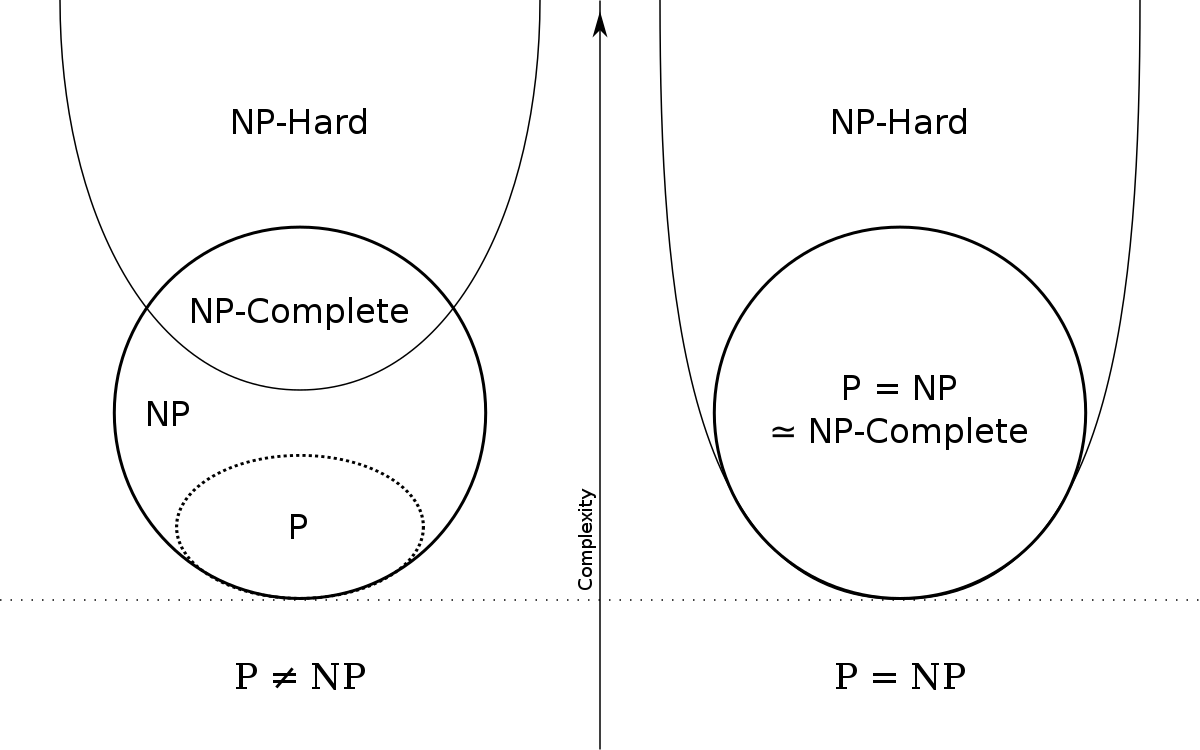
\includegraphics[scale = 0.3]{img/problem.png}
  \caption{Diagramma di \emph{Eulero Venn} per le classi di complessità}
  \label{fig:complexity}
\end{figure}
\begin{shaded}
  \textit{Tratto dagli appunti di Metodi Formali:}\\
\begin{center}
  \textit{Si parla di isomorfismo quando due strutture complesse si possono
    applicare l'una sull'altra, cioè far corrispondere l'una all'altra, in modo
    tale che per ogni parte di una delle strutture ci sia una parte
    corrispondente nell'altra struttura; in questo contesto diciamo che due
    parti sono corrispondenti se hanno un ruolo simile nelle rispettive
    strutture.}
\end{center}
Diamo ora una definizione formale di isomorfismo tra sistemi di transizione
etichettati, che possono quindi essere grafi dei casi o grafi dei casi
sequenziali.
\begin{definizione}
  Siano dati due sistemi di transizione etichettati:\\
  $A_1 = (S_1,E_1,T_1,s_{01})$ e $A_2 = (S_2 , E_2 , T_2 , s_{02})$.\\
  e siano date due \textbf{mappe biunivoche}:
  \begin{enumerate}
    \item $\alpha:S_1\to S_2$, ovvero che passa dagli stati del primo sistema a
    quelli del secondo
    \item $\beta:E_1\to E_2$, ovvero che passa dagli eventi del primo sistema a
    quelli del secondo
  \end{enumerate}
  allora:
  \[\langle \alpha,\beta\rangle:A_1= (S_1 , E_1 , T_1 ,s_{01})\to A_2 = (S_2 ,
    E_2 , T_2 , s_{02})\]
  è un \textbf{isomorfismo} sse:
  \begin{itemize}
    \item $\alpha(s_{01})=s_{02}$, ovvero l'immagine dello stato iniziale del
    primo sistema coincide con lo stato iniziale del secondo
    \item $\forall s,s'\in S_1,\forall e\in E_1:\,(s,e,s')\in T_1
    \Leftrightarrow (\alpha(s),\beta(e),\alpha(s'))\in T_2$ ovvero per ogni
    coppia di stati del primo sistema, tra cui esiste un arco etichettato $e$,
    vale che esiste un arco, etichettato con l'immagine di $e$, nel secondo
    sistema che va dall'immagine del primo stato considerato del primo sistema
    all'immagine del secondo stato considerato del secondo sistema, e viceversa
  \end{itemize}
\end{definizione}
\begin{definizione}
  Si definiscono due \textbf{sistemi equivalenti} sse hanno grafi dei casi
  sequenziali, e quindi di conseguenza anche grafi dei casi, \emph{isomorfi}.\\
  Due sistemi equivalenti accettano ed eseguono le stesse sequenze di eventi
\end{definizione}
\end{shaded}
\section{Riduzioni polinomiali}
Si hanno alcuni problemi che sono in grado di risolvere qualunque problema di
decisione in \textbf{NP}. Serviranno prima le definizioni di \textbf{NP-hard} e
\textbf{NP-complete}.\\
Vediamo innanzitutto il problema \textit{independent-set} che ci aiuterà
analisi.
\begin{definizione}
  L'\textit{independent-set } di un grafo non orientato è un sottoinsieme
  $I\subseteq V$ tale che $\forall u,v\in I$ $(u,v)\not\in E$. Il problema
  \textit{ind\_set}, nella versione di ottimo, è quello di trovare
  l'\textit{independent-set} di cardinalità massima di un grafo non
  orientato. Nella versione di decisione $ind\_set_d$ si ha anche il parametro
  $k$ intero e si cerca se esiste un \textit{independent-set} di cardinalità
  uguale a $k$. L'\textit{independent-set} di cardinalità massima può essere
  usato come ``certificato''.
\end{definizione}
Questo problema è legato alla \textit{copertura dei vertici}, infatti sappiamo
che se dall'insieme dei vertici togliamo un sottoinsieme di minima copertura
troviamo un \textit{independent-set} di cardinalità massima perché sto facendo
il complemento di un insieme di copertura di cardinalità minima, infatti tra i
vertici non nell'insieme di copertura di cardinalità minima, ovvero nel
complemento, non posso avere un arco per definizione e quindi se il primo è di
cardinalità minima allora il secondo, che è l'\textit{independent-set}, è di
cardinalità massima. Infatti i vertici nella copertura sono vertici che toccano
tutti gli archi.\\
Dal punto di vista delle applicazioni pratiche questi problemi si prestano allo
studio, per esempio, delle telecomunicazioni.
\begin{proof}
  Dimostriamo che $ind\_set_d$ è \textbf{NP}, infatti esiste un algoritmo $A$
  che in costo polinomiale prende in ingresso il grafo, $k$, e un
  ``certificato'' $y$ e i vertici in $y$, che sono vertici di un
  \textit{independent\_set} per il grafo $G$ di cardinalità $k$. L'algoritmo
  verifica che $y$ è un \textit{independent-set} e il costo della verifica è
  quadratico su $|y|$, ovvero $|y|^2$ che nel caso peggiore è $|V|^2$. So anche
  che, per l'input $x$, $O(|x|)=O(|E|+|V|)=O(|V^2|+|V|)$ nel caso peggiore,
  quindi il tempo di verifica è \textbf{polinomiale}.
\end{proof}
\begin{definizione}
  Vediamo ora il problema di \textbf{soddisfacibilità} $SAT$. Questo problema
  prende in input una formula booleana $\phi$ in \textbf{forma normale congiunta
    (CNF)}, ovvero che ha una congiunzione ($\land$) come legame tra le
  \textbf{clausole}. Una clausola è un $\lor$ di \textbf{letterali}, ovvero di
  variabili booleane $x_i$ o $\neg x_i$. In output ho se la forma sia
  soddisfacibile o meno. 
  \begin{esempio}
    Prendo 3 variabili, $x_1,x_2,x_3$. Creo i letterali  $x_1,x_2,x_3$ e anche
    $\neg x_1,\neg x_2,\neg x_3$. Creo quindi le clausole $c_1=x_1\lor x_2$,
    $c_2=x_1\lor \neg x_2$ e $c_3=x_1\lor \neg x_2$. Definisco quindi la CNF
    $\phi$:
    
    \[\phi=(x_1\lor x_2)\land (x_1\lor \neg x_2)\land
      (x_1\lor \neg x_2)=c_1\land c_2\land c_3\]
    Quindi in ogni clausola almeno un letterale deve essere vero, cosicché tutte
    le clausole siano vere rendendo vera la CNF.\\
    Avendo due letterali a clausola si è definito un $2SAT$.
  \end{esempio}
  Il numero di letterali $k$ che compongono la clausola definsice un problema
  $kSAT$. Si ha che $2SAT\in P$ ma con $k>2$ si ha che $kSAT\in NP$ (in
  realtà è in \textbf{NP-hard})
\end{definizione}
\begin{definizione}
  Definiamo un problema \textbf{NP-hard} come un problema difficile almeno
  quanto un problema \textbf{NP}. Ogni che problema $A$ in \textbf{NP} può
  essere risolto con un chiamata di procedura a $B$, che è un problema
  \textbf{NP-hard} a cui tutti gli altri ``chiedono aiuto'' per trovare una
  soluzione. \\
  Ad esempio \textit{vertex-cover} è un problema \textbf{NP-hard} e quindi posso
  risolvere ogni problema $A$ in \textbf{NP} con il problema
  \textit{vertex-cover} $B$.\\
  Trasformo quindi l'input $w$ di $A$ in un input
  $f(w)$ per $B$ in tempo polinomiale. La risposta di $B$ con input $f(w)$ è la
  stessa che $A$ da su input $w$.\\
  Non tutti i problemi \textbf{NP-hard} sono dentro la classe \textbf{NP}
\end{definizione}
\begin{definizione}
  Definiamo quindi il concetto di \textbf{riduzione}, rappresentato in figura
  \ref{fig:rid}.\\
  La riduzione è la trasformazione dell'input di $w$ in $A$ in un input $f(w)$
  per $B$, in tempo polinomiale. La risposta di $B$ con input $f(w)$ è la stessa
  che $A$ da su input $w$.\\
  Si ha che $A$ si riduce polinomialmente a $B$, e si scrive:
  \[A\leq_p B\]
  se $\exists\,f$ tale che:
  \[w \in L_A\mbox{ sse } f(w)\in L_B\]
  con $f$ calcolabile in tempo polinomiale, infatti il calcolo di $f(w)$ è
  $=(|w|^p)$, con $p\in\mathbb{N}$ per semplicità. Non devo introdurre una
  complessità superiore nel contesto di confronto tra problemi (??).\\ 
  \begin{figure}
    \centering
    
    \psscalebox{0.9 0.9} % Change this value to rescale the drawing.
    {
      \begin{pspicture}(0,-2.8)(15.0,2.8)
        \definecolor{colour1}{rgb}{0.34901962,0.6627451,0.3019608}
        \definecolor{colour0}{rgb}{0.8784314,0.20392157,0.20392157}
        \definecolor{colour2}{rgb}{0.3254902,0.38039216,0.99607843}
        \psframe[linecolor=colour1, linewidth=0.04, dimen=outer]
        (13.52,2.8)(1.52,-2.8)
        \psframe[linecolor=colour0, linewidth=0.04, dimen=outer]
        (6.32,1.2)(2.72,-1.2)
        \psframe[linecolor=colour0, linewidth=0.04, dimen=outer]
        (6.32,1.2)(2.72,-1.2)
        \psframe[linecolor=colour2, linewidth=0.04, dimen=outer]
        (11.52,1.2)(7.92,-1.2)
        \psline[linecolor=black, linewidth=0.04, arrowsize=0.05291667cm 2.0,
        arrowlength=1.4,arrowinset=0.0]{->}(6.32,0.0)(7.92,0.0)
        \psline[linecolor=black, linewidth=0.04, arrowsize=0.05291667cm 2.0,
        arrowlength=1.4,arrowinset=0.0]{->}(0.72,0.0)(2.72,0.0)
        \psline[linecolor=black, linewidth=0.04, arrowsize=0.05291667cm 2.0,
        arrowlength=1.4,arrowinset=0.0]{->}(11.52,0.4)(14.32,0.4)
        \psline[linecolor=black, linewidth=0.04, arrowsize=0.05291667cm 2.0,
        arrowlength=1.4,arrowinset=0.0]{->}(11.52,-0.4)(14.32,-0.4)
        \rput[bl](3.7,1.3){Riduzione}
        \rput[bl](0.0,-0.14){$w$}
        \rput[bl](4.1,-0.08){$f(w)$}
        \rput[bl](9.42,-0.08){$B$}
        \rput[bl](12.26,0.6){yes}
        \rput[bl](14.42,0.25){yes}
        \rput[bl](12.34,-0.74){no}
        \rput[bl](14.42,-0.5){no}
        \rput[bl](9.24,1.3){$SAT$}
        \rput[bl](6.72,0.4){$f(w)$}
      \end{pspicture}
    }
    \caption{Rappresentazione grafica della riduzione}
    \label{fig:rid}
  \end{figure}
  Ogni problema $A$ che in \textbf{NP} può essere risolto con una chiamata di
  procedura a $B$, quindi posso risolvere ogni problema $A\in NP$ con
  \textit{vertex-cover}, essendo esso un problema \textbf{NP-hard}.
  
\end{definizione}
\begin{definizione}
  $B$ è \textbf{NP-hard} sse $\forall A\in NP$ $A$ si riduce a $B$ in tempo
  polinomiale:
  \[A\leq_p B,\,\,\forall A\]
  Un problema $NP-hard$ può non essere in $NP$, in quanto potrebbe non avere un
  ``certificato'' per consentire la verifica in tempo polinomiale.
\end{definizione}
\begin{definizione}
  Un problema \textbf{NP-hard} e anche \textbf{NP} si dice che il problema è
  \textbf{NP-complete} 
\end{definizione}
$kSAT$ è il primo problema che si è dimostrato essere anche
\textbf{NP-complete}.
\begin{esempio}
  Vediamo un esempio di riduzione, rappresentata in figura \ref{fig:ride}:
  \[3SAT\leq_p ind\_set_d\]
  arrivando e alla conclusione che $ind\_set_d$ è \textbf{NP-completo}.\\
  \begin{figure}
    \centering
    
    \psscalebox{0.9 0.9} % Change this value to rescale the drawing.
    {
      \begin{pspicture}(0,-2.8)(15.0,2.8)
        \definecolor{colour1}{rgb}{0.34901962,0.6627451,0.3019608}
        \definecolor{colour0}{rgb}{0.8784314,0.20392157,0.20392157}
        \definecolor{colour2}{rgb}{0.3254902,0.38039216,0.99607843}
        \psframe[linecolor=colour1, linewidth=0.04, dimen=outer]
        (13.52,2.8)(1.52,-2.8)
        \psframe[linecolor=colour0, linewidth=0.04, dimen=outer]
        (6.32,1.2)(2.72,-1.2)
        \psframe[linecolor=colour0, linewidth=0.04, dimen=outer]
        (6.32,1.2)(2.72,-1.2)
        \psframe[linecolor=colour2, linewidth=0.04, dimen=outer]
        (11.52,1.2)(7.92,-1.2)
        \psline[linecolor=black, linewidth=0.04, arrowsize=0.05291667cm 2.0,
        arrowlength=1.4,arrowinset=0.0]{->}(6.32,0.0)(7.92,0.0)
        \psline[linecolor=black, linewidth=0.04, arrowsize=0.05291667cm 2.0,
        arrowlength=1.4,arrowinset=0.0]{->}(0.72,0.0)(2.72,0.0)
        \psline[linecolor=black, linewidth=0.04, arrowsize=0.05291667cm 2.0,
        arrowlength=1.4,arrowinset=0.0]{->}(11.52,0.4)(14.32,0.4)
        \psline[linecolor=black, linewidth=0.04, arrowsize=0.05291667cm 2.0,
        arrowlength=1.4,arrowinset=0.0]{->}(11.52,-0.4)(14.32,-0.4)
        \rput[bl](3.7,1.3){Riduzione}
        \rput[bl](0.35,-0.15){$\phi$}
        \rput[bl](4.1,-0.08){$f(\phi)$}
        \rput[bl](9.42,-0.08){$B$}
        \rput[bl](14.42,0.25){1}
        \rput[bl](14.42,-0.5){0}
        \rput[bl](9.0,1.3){$ind\_set_d$}
        \rput[bl](6.85,0.2){$G_\phi$}
      \end{pspicture}
    }
    \caption{Rappresentazione grafica del'esempio \ref{es:1}}
    \label{fig:ride}
  \end{figure}
  e vediamo che $\phi$ è soddisfacibile sse $G_\phi$ ha un
  \textit{independent-set} di dimensione $k=|\phi|$, con $|\phi|$ pari al numero
  di clausole della formula.\\
  Costruisco quindi un grafo che ha un vertice per ogni letterale della
  clausola. Collego i tre letterale della clausola ottenendo un
  ``triangolo'', detto \textit{gadget}, che rappresenta una clausola. Infine
  collego ogni letterale al suo negato.
  \newpage
  Quindi per la formula:
  \[\phi=(\neg x_1\lor x_2\lor x_3)\land(x_1\lor \neg x_2\lor x_3)\land(\neg
    x_1\lor x_2\lor x_4)\]
  avrò il grafo $G_\phi$ che codifica la formula $\phi$:
  \begin{figure}[H]
    \centering
    \psscalebox{1.0 1.0} % Change this value to rescale the drawing.
    {
      \begin{pspicture}(0,-1.5798438)(12.92,1.5798438)
        \pscircle[linecolor=black, linewidth=0.04, fillstyle=solid,
        fillcolor=black, dimen=outer](1.6,0.9050586){0.4}
        \pscircle[linecolor=black, linewidth=0.04, fillstyle=solid,
        fillcolor=black, dimen=outer](0.4,-0.6949414){0.4}
        \pscircle[linecolor=black, linewidth=0.04, fillstyle=solid,
        fillcolor=black, dimen=outer](2.8,-0.6949414){0.4}
        \psline[linecolor=black, linewidth=0.02](1.6,0.5050586)(2.4,-0.6949414)
        \psline[linecolor=black, linewidth=0.02](1.6,0.5050586)(0.8,-0.6949414)
        \psline[linecolor=black, linewidth=0.02](0.8,-0.6949414)(2.4,-0.6949414)
        \rput[bl](1.2,1.3050586){$\neg x_1$}
        \rput[bl](2.6,-1.4949414){$x_3$}
        \rput[bl](0.2,-1.4949414){$x_2$}
        \pscircle[linecolor=black, linewidth=0.04, fillstyle=solid,
        fillcolor=black, dimen=outer](6.4,0.9050586){0.4}
        \pscircle[linecolor=black, linewidth=0.04, fillstyle=solid,
        fillcolor=black, dimen=outer](5.2,-0.6949414){0.4}
        \pscircle[linecolor=black, linewidth=0.04, fillstyle=solid,
        fillcolor=black, dimen=outer](7.6,-0.6949414){0.4}
        \psline[linecolor=black, linewidth=0.02](6.4,0.5050586)(7.2,-0.6949414)
        \psline[linecolor=black, linewidth=0.02](6.4,0.5050586)(5.6,-0.6949414)
        \psline[linecolor=black, linewidth=0.02](5.6,-0.6949414)(7.2,-0.6949414)
        \rput[bl](6,1.3050586){$\neg x_2$}
        \rput[bl](7.4,-1.4949414){$x_3$}
        \rput[bl](5.0,-1.4949414){$x_1$}
        \pscircle[linecolor=black, linewidth=0.04, fillstyle=solid,
        fillcolor=black, dimen=outer](11.2,0.9050586){0.4}
        \pscircle[linecolor=black, linewidth=0.04, fillstyle=solid,
        fillcolor=black, dimen=outer](10.0,-0.6949414){0.4}
        \pscircle[linecolor=black, linewidth=0.04, fillstyle=solid,
        fillcolor=black, dimen=outer](12.4,-0.6949414){0.4}
        \psline[linecolor=black,linewidth=0.02](11.2,0.5050586)(12.0,-0.6949414)
        \psline[linecolor=black,linewidth=0.02](11.2,0.5050586)(10.4,-0.6949414)
        \psline[linecolor=black,linewidth=0.02]
        (10.4,-0.6949414)(12.0,-0.6949414)
        \rput[bl](10.8,1.3050586){$\neg x_1$}
        \rput[bl](12.2,-1.4949414){$x_4$}
        \rput[bl](9.8,-1.4949414){$x_2$}
        \psline[linecolor=black, linewidth=0.02](0.8,-0.6949414)(6.0,0.9050586)
        \psline[linecolor=black, linewidth=0.02](2.0,0.9050586)(4.8,-0.6949414)
        \psline[linecolor=black, linewidth=0.02](5.6,-0.6949414)(10.8,0.9050586)
        \psline[linecolor=black, linewidth=0.02](6.8,0.9050586)(9.6,-0.6949414)
      \end{pspicture}
    }
    \label{es:1}
  \end{figure}
  Quindi un \textbf{gadget} è una rappresentazione dell'input del problema $A$
  di partenza e ogni \textbf{gadget} rappresenta una clausola.\\
  Ricordiamo che $\phi$ è soddisfacibile sse esiste un assegnamento delle
  variabili della formula tale per cui almeno un letterale di ogni clausola è
  vero. Nel grafo relativo alla formula lego quindi un letterale ad ogni suo
  complemento al fine di poter identificare i valori di verità e avendo il
  calcolo di \textit{independent-set} (per la \textbf{riduzione}) prendo uno
  solo degli estremi di un arco, e quindi uno solo tra $x_i$ e $\neg x_i$,
  codificando l'assegnamento di verità. Il concetto di \textbf{riduzione} è
  quindi ritrovabile nella capacità di rappresentare un problema in un'altra
  forma, studiabile con un altro algoritmo.
  \begin{proof}
    Indichiamo con $A$ $3SAT$ e con $B$ \textit{independent-set}.\\
    Effettuiamo quindi la prova finale, la dimostrazione vera e propria. A
    questo livello di comprensione abbiamo dimostrato
    l'esistenza della funzione $f$, che trasforma $\phi$ (ovvero l'input di $A$)
    in $\langle G, k\rangle$, ovvero l'input di $B$, e che essa è in tempo
    polinomiale. Abbiamo quindi che $w\in L_A$ sse $f(w)\in L_B$. Se $\phi$ è
    vera allora esiste un \textit{independent-set} di dimensione $k$ per
    $\langle G, k\rangle$.\\ 
    Nell'\,''altro verso'' abbiamo che se esiste un \textit{independent-set} di
    dimensione $k$ per $\langle G, k\rangle$ allora $\phi$ è vera. Dimostrare
    questi due ``versi'' equivale a dimostrare la riduzione.\\
    Il \textbf{primo verso} si dimostra dicendo che dato un assegnamento di
    verità si seleziona un letterale vero da ogni triangolo. Questi letterali
    veri scelti formano l'\textit{independent-set} $S$, che ha dimensione
    $k$. Questo può accadere sse $\phi$ è vera, infatti per ogni clausola $c_i$
    $\exists \,\,l_{ij}$, letterale, che rende vera $c_i$, a questo punto tale
    letterale è un vertice del triangolo, ovvero del gadget $g_{c_i}$, (mi basta
    infatti un letterale vero per triangolo) e, poiché
    tutte le clausole sono vere, ho la scelta di $k$ vertici se $k$ è il numero
    delle clausole. Esiste quindi un \textit{independent-set} di dimensione
    $k$.\\
    Per questo si potrebbe fare una \textbf{dimostrazione per costruzione},
    ovvero se rendo vera $c_y$ con $l_y$ significa che la variabile $x_i$ può
    essere usata o come 1 o come 0 nell'assegnamento di verità in un altro
    letterale $l_z$, che rende vera la clausola $c_z$. Ma $x_i$, se già usata,
    non posso più usarla con valore opposto a quello scelto per $c_y$ e quindi
    non esiste un arco di collegamento tra $l_y$ e $l_z$.\\
    Si può dimostrare anche per \textbf{assurdo}. Se esiste un arco tra i due
    letterali $l_z$ e $l_y$ che rendono vere le clausole $c_z$ e $c_y$,
    allora ottengo una contraddizione sugli assegnamenti di verità, asserendo
    che i due letterali sono uno la negazione dell'altro ma entrambi sono
    veri, per poter rendere vere le clausole. 
    \\
    \\
    Il \textbf{secondo verso} si dimostra dicendo che, dato un
    \textit{independent-set} 
    $S$ di dimensione $k$, $S$ deve contenere un vertice per triangolo. Ponendo
    quindi i letterali contenuti in $S$ come veri si ottiene un assegnamento di
    verità che è \textbf{consistente} e tutte le clausole sono soddisfatte.
    Quindi se esiste un \textit{independent-set} di dimensione $k$ allora trovo
    un assegnamento alle variabili $x_i,\,\,\forall \,\,1\ldots n$ che rende
    vera $\phi$, ovvero assegno 0 o 1 a ciascuna variabile (ovviamente o 1 o 0,
    non entrambi). Se esiste l'\textit{independent-set} di dimensione $k$ pari
    al numero delle clausole, allora per ogni gadget $g_{c_i}$,
    che rappresenta una clausola, esiste un vertice nel gadget che si trova
    anche nell'\textit{independent-set}, quindi esiste un letterale, per ogni
    clausola $c_i$ tale che non è collegato ad un altro letterale
    dell'\textit{independent-set}, ovvero non è collegato ad un altro letterale
    di un'altra clausola (ovvero ho un nodo per gadget che non ha un arco verso
    un nodo di un altro gadget). Quindi per ogni letterale vedo la variabile che
    rende vero il letterale e con il valore dato alla variabile costruisco
    l'assegnamento o 0 o 1 a quella variabile (se $l_i=\neg x_j$ allora
    $x_j=0$ e se $l_i= x_j$ allora $x_j=1$). Trovo quindi l'assegnamento delle
    variabili che è di verità per $\phi$, dimostrando quindi che $\phi$ è vera.
  \end{proof}
\end{esempio}
Siccome $3SAT$ è \textbf{NP-complete} allora anche \textit{independent-set} è
\textbf{NP-complete}, infatti:
\[\forall\,\, A_{\in NP}\leq_p 3SAT\leq_p \mbox{ \textit{independent-set}}\]
in quanto la riduzione $\leq_p$ è \textbf{transitiva}, e quindi:
\[\forall\,\, A_{\in NP}\leq_p \mbox{ \textit{independent-set}}\in NP\]
\begin{teorema}
  Se un problema $\Pi$ \textbf{NP-complete} è in \textbf{P} allora si può dire
  $P=NP$, implicando che ogni problema $A\in NP$ è risolvibile da $\Pi\in P$.
  Questa cosa non è stata ancora dimostrata (e probabilmente si riuscirà
  a dimostrare l'opposto).
\end{teorema}
\begin{proof}
  Per ogni problema $A$ in \textbf{NP} so che $A\leq_p \Pi$, ovvero $\Pi$ è una
  procedura che risolve $A$, con trasformazione dell'input $x$ di $A$ nell'input
  $f(x)$ di $\Pi$, con $f(x)$ calcolabile in tempo polinomiale.\\
  Assumendo quindi che $\Pi\in P$ allora anche ogni $A\in P$, e quindi $NP=P$.
\end{proof}
\begin{teorema}
  La riduzione polinomiale è transitiva. Ovvero se $A\leq_p B$ e $B\leq_p C$
  allora:
  \[A\leq_p C\]
\end{teorema}
\begin{proof}
  Infatti $A\leq_p B$ implica l'esistenza di $f$ tale che $x\in L_A$ sse
  $f(x)=L_B$. Ugualmente $B\leq_p C$ implica l'esistenza di $g$ tale che $x\in
  L_B$ sse $g(x)=L_C$.\\
  Devo dimostrare che $\exists\,\,f'$ tale che $x\in L_A$ sse $f'(x)\in
  L_C$. Per ottenere $f'$ compongo $f$ e $g$. Assumendo che $x$ appartiene
  all'input di ha compongo le funzioni, quindi ho che $f'=g\circ f$,
  e ho che $x\in L_A$ e che $f(x)\in L_B$ (quindi $f(x)$ è un input per $B$) ma
  quindi $g(f(x))\in L_C$ (quindi $g(f(x))$ è un input per $C$). Ho quindi
  dimostrato la transitività.\\
  Se $f$ e $g$ sono costruibili in tempo polinomiale, la prima sulla dimensione
  di $x$ e la seconda su quella di $f(x)$, allora anche $f'=g\circ f$
  è costruibile in tempo polinomiale, proporzionalmente alla cardinalità di $x$.
\end{proof}
Quindi per dimostrare che un problema $\Pi'$ è \textbf{NP-hard} devo ridurre
$\Pi'$ ad un problema qualsiasi \textbf{NP-hard} (in base alla somiglianza del
problema), sapendo che $\forall A\in NP$ $A$ si riduce ad un problema
\textbf{NP-hard}, come $SAT$.\\
In modo equivalente per dire che è un problema è \textbf{NP-complete} faccio
quanto fatto per \textbf{NP-hard} ma devo aggiungere che esso sia in $NP$,
dovendo quindi aggiungere il ``certificato''.
% immagine slide 6(teorema cook)
\begin{teorema}
  Si ha che $SAT\leq_p 3SAT$
\end{teorema}
\begin{proof}
  \textbf{Dimostrazione solo parziale, solo l'inizio è stato fatto in aula.\\}
  Prendo una $\phi$ con $k\geq 4$ letterali. Ogni clausola deve diventare una
  clausola con al più 3 letterali (introducendo nuovi letterali ogni volta che
  viene negato uno). 
\end{proof}
\subsection{Problema set-cover}
Questo problema si applica bene allo studio, nel campo delle telecomunicazioni,
dei ripetitori e dello studio della copertura per reti mobili.
\begin{definizione}
  Dato un universo $U$ di $n$ elementi sia $S=\{S_1,\ldots,S_M\}$ una collezione
  di sottoinsiemi di $U$. Sia anche data una funzione di costo
  $c:S\to\mathbb{Q}^+$. Il problema \textbf{set-cover} consiste nel trovare una
  collezione $C$ di sottoinsiemi di $S$ di costo minimo che copra tutti gli
  elementi di $U$.
\end{definizione}
\begin{esempio}
  Se ho $U=\{1,2,3,4,5\}$, $S_1=\{1,2,3\}$, $S_2=\{2,3\}$, $S_3=\{4,5\}$ e
  $S_4=\{1,2,4\}$, con $S=\bigcup S_i$ . Per praticità assumo costo
  uniforme, ovvero che  $c_1=c_2=c_3=c_4=1$.\\
  Quindi la soluzione $C$ è $\{S_1,S_3\}$, in quanto questi due insiemi coprono
  tutti gli elementi di $U$, con costo pari a $5$ (che è il minimo che posso
  avere).
\end{esempio}
\begin{definizione}
  Qualora il costo sia uniforme allora il \textbf{set-cover} diventa la ricerca
  di una sotto-collezione che copra tutti gli elementi di $U$ con minima
  dimensione.
\end{definizione}

\begin{teorema}
  \textit{set-cover}, nella versione decisionale e nella
  versione con peso uniforme, è \textbf{NP-complete} (quindi se esiste una
  collezione $C$ di sottoinsiemi di $S$ 
  la cui unione sia $U$ con cardinalità minore uguale di $k$).
\end{teorema}
\begin{proof}
  Posso facilmente dimostrare che $|C|\leq k$ in tempo polinomiale e che
  l'unione degli insieme di $C$ include tutti gli elementi di $U$, in
  tempo polinomiale su $|U|$. Posso aggiungere anche un ``certificato'', nella
  forma di una collezione che copre tutto $U$ (e quindi la verifica è in tempo
  polinomiale sulla dimensione del ``certificato'' più quella di $U$). Quindi
  \textbf{set-cover} è in \textbf{NP}.\\
  Per dimostrare che \textbf{set-cover} è \textbf{NP-hard} dimostro che:
  \[\mbox{vertex-cover} \leq_p \mbox{set-cover}\]
  ovvero uso un problema che so già essere \textbf{NP-hard}, appunto
  \textit{vertex-cover} (avendo già dimostrato che $\forall A\in NP, \,\,A\leq_p
  \mbox{vertex-cover}$, dimostrando che \textit{set-cover} dimostra tutti i
  problemi in \textbf{NP}).\\
  Faccio vedere che posso usare \textit{set-cover} per dimostrare
  \textit{vertex-cover}.\\
  Devo quindi trasformare un'istanza di \textit{vertex-cover} $C=\langle
  G=(V,E), j\rangle$ in un'istanza $C'$ di \textit{set-cover}, in tempo
  polinomiale, tale che $C$ è soddisfacibile sse $C'$ è soddisfacibile.\\
  Procedo quindi con la trasformazione. Pongo innanzitutto $U=E$. Per quanto
  riguarda la collezione $S$ procedo nel seguente modo. Etichetto i vertici in
  $V$ da $1$ a $n$. A questo punto $S_i$ diventa l'insieme degli archi incidenti
  al vertice $i$-simo. A questo punto basta porre $k=j$ per concludere la
  costruzione polinomiale dell'istanza di \textit{set-cover}.\\
  In poche parole ciascun arco è un elemento di $U$ e ciascun vertice è un
  insieme di $S$.\\
  Vediamo anche la dimostrazione formale che \textit{vertex-cover} risponde
  ``yes'', per $j$, sse istanza di \textit{set-cover} risponde ``yes'' per
  $k=j$.\\
  Innanzitutto se \textit{vertex-cover} risponde ``yes'' per $j$ allora trovo
  una collezione di \textit{set-cover} buona di cardinalità $j$. Suppongo
  infatti $G$ ha una copertura C di al più $j$ vertici e quindi $C$ corrisponde
  ad una collezione di $C'$ di sottoinsiemi $U$. Poiché assumo $k=j$ allora
  $|C'|\leq k$. Inoltre $C'$ copre tutti gli elementi di $U$ coprendo tutti gli
  archi di $G$, in quanto ogni elemento di $U$ è un arco in $G$. Poiché $C$ è
  una copertura, almeno un estremo dell’arco è in $C$  e quindi l’arco è in un
  insieme di $C'$.\\
  Dimostriamo anche l'altro verso della dimostrazione, ovvero devo garantire
  l'esistenza della copertura. Suppongo di avere un set cover $C'$ di dimensione
  $k$. Dato che ad ogni insieme di $C'$ ho associato un vertice in $G$ allora
  $|C|=|C'|\leq k=j$. Inoltre, $C$ è una copertura di $G$ poiché $C'$ è un
  set-cover, poiché, preso un arco $e$ ho che $e\in U$ e quindi $C'$ deve
  contenere almeno un insieme che contiene $e$ e tale insieme è quello che
  corrisponde ai nodi che sono estremi di $e$. Quindi $C$ deve contenere almeno
  un estremo di $e$. Quindi posso concludere dicendo che $C$ è copertura di $G$.
\end{proof}
Si continua la ricerca di una dimostrazioni di \textbf{NP-completezza}, ambito
di studio nato dopo la scoperta di Cook di $SAT\in$ \textbf{NP-complete}.\\
Partiamo ricordando che:
\begin{teorema}
  Se $B$ è un problema tale che $A\leq_p B$, con $A$
  \textbf{NP-hard} (o ovviamente anche \textbf{NP-complete}), allora $B$ è
  \textbf{NP-hard} e se inoltre $B\in NP$ allora $B$ è \textbf{NP-complete}.  
\end{teorema}
\begin{proof}
  Con la transitività della riduzione $\leq_p$ si ha che $\forall\pi\in
  NP,\,\,\, \pi\leq_p A$ e quindi $A$ è \textbf{NP-hard}. Inoltre avendo
  $A\leq_p B$ ho che  $\pi\leq_p B$ e quindi $B$ è \textbf{NP-hard}, inoltre,
  avendo $B\in NP$, ho che è \textbf{NP-complete}
\end{proof}


\subsection{Problemi di ottimizzazione}
\subsubsection{Clique-problem}
\begin{definizione}
  Definisco \textbf{clique (\textup{cricca})} di un grafo non orientato
  $G=(V,E)$ come un sottoinsieme $V'\subseteq V$ di vertici tale che:
  \[\forall \,v_1,v_2\in V' (v_1,v_2)\in E\]
  quindi un sottoinsieme di vertici con solo vertici collegati da un arco.
\end{definizione}
Definisco quindi il problema.
\begin{definizione}
  Il \textbf{clique-problem} è un problema di ottimizzazione (nel
  dettaglio di massimo) in cui si cerca la \textbf{clique} di dimensione massima
  di un grafo (ovvero $|V'|$ è massimo). Nella versione decisionale chiedo se
  esiste una \textbf{clique} di dimensione $k$.\\
  Il problema è \textbf{NP-complete}
\end{definizione}
\begin{proof}
  Dimostriamo che sia \textbf{NP-complete} (nella versione decisionale). Cerco
  quindi un algoritmo 
  polinomiale, con``certificato''. Uso quindi un insieme $V'\subseteq V$ come
  vertici della \textbf{clique} come ``certificato'' per il grafo in input. Per
  verificare che $V'$ è una \textbf{clique} controllo che:
  \[\forall\,v_1,v_2\in    V' (v_1,v_2)\in E\]
  e questa verifica è polinomiale, infatti è $O(|V'|^2)$ e
  quindi è quadratico nella dimensione dell'input.\\
  Bisogna ora trovare un problema $A\in \mbox{NP-complete}$ tale che $A$ si
  riduce in tempo polinomiale al \textbf{clique-problem} (quindi
  \textbf{clique-problem} risolve $A$).  \\
  Notiamo che una \textbf{clique} è l'opposto di \textbf{independent-set}, che
  avevamo dimostrato tramite $3SAT$ (che può risolvere
  \textbf{independent-set}).\\
  Quindi per \textbf{clique-problem} provo ancora ad usare $3SAT$. Devo fare in
  modo che $\phi\in 3SAT$ sse il grafo $G_\phi$ ha una \textbf{clique} di
  dimensione uguale al numero di clausole di $\phi$. Quindi avendo $k$ clausole
  in $\phi$ avrò che ciascuna clausola sarà un gadget e da ogni gadget estrarrà
  un vertice che comporrà la \textbf{clique} di dimensione $k$.\\
  Il grafo $G_\phi$ è costruito come nel caso di \textit{independent-set} coi
  letterali come vertici.\\
  Bisogna studiare il collegamento tra tali vertici (che sarà diverso al caso di
  \textit{independent-set}, non avendo quindi i triangoli).\\
  Ipotizzo:
  \[\phi=c_1\land c_2\land c_3\]
  con:
  \[c_1=x_1\lor \neg x_2\lor \neg x_3\]
  \[c_2=\neg x_1\lor x_2\lor x_3\]
  \[c_3=x_1\lor x_2\lor x_3\]
  Per ogni clausola faccio i vertici per ogni letterale (distinti anche per lo
  stesso letterale, come nel caso di \textit{independent-set}).\\
  Per ora abbiamo vertici isolati e i tre vertici isolati di ogni clausola sono
  il gadget. A questo punto collego ogni letterale di ogni clausola con ogni
  altro letterale di ogni altra clausola (non della stessa) che non sia
  l'opposto, collegando quindi solo vertici \textbf{consistenti} (in quanto non
  potrei avere una \textbf{clique} connettendo due vertici non consistenti). Sto
  facendo esattamente l'opposto di \textit{independent-set}. 
  \begin{figure}
    \centering
    \psscalebox{0.9 0.9} % Change this value to rescale the drawing.
    {
      \begin{pspicture}(0,-4.3798437)(8.58,4.3798437)
        \definecolor{colour0}{rgb}{0.003921569,0.003921569,0.003921569}
        \pscircle[linecolor=black, linewidth=0.04,
        fillstyle=solid,fillcolor=colour0, dimen=outer](2.8,3.3050585){0.4}
        \pscircle[linecolor=black, linewidth=0.04,
        fillstyle=solid,fillcolor=colour0, dimen=outer](6.8,3.3050585){0.4}
        \pscircle[linecolor=black, linewidth=0.04,
        fillstyle=solid,fillcolor=colour0, dimen=outer](4.8,3.3050585){0.4}
        \pscircle[linecolor=black, linewidth=0.04,
        fillstyle=solid,fillcolor=colour0, dimen=outer](1.2,2.1050587){0.4}
        \pscircle[linecolor=black, linewidth=0.04,
        fillstyle=solid,fillcolor=colour0, dimen=outer](1.2,-1.8949414){0.4}
        \pscircle[linecolor=black, linewidth=0.04,
        fillstyle=solid,fillcolor=colour0, dimen=outer](1.2,0.105058596){0.4}
        \pscircle[linecolor=black, linewidth=0.04,
        fillstyle=solid,fillcolor=colour0, dimen=outer](2.8,-3.0949414){0.4}
        \pscircle[linecolor=black, linewidth=0.04,
        fillstyle=solid,fillcolor=colour0, dimen=outer](6.8,-3.0949414){0.4}
        \pscircle[linecolor=black, linewidth=0.04,
        fillstyle=solid,fillcolor=colour0, dimen=outer](4.8,-3.0949414){0.4}
        \rput[bl](2.65,3.9050587){$x_1$}
        \rput[bl](4.4,3.9050587){$\neg x_2$}
        \rput[bl](6.4,3.9050587){$\neg x_3$}
        \rput[bl](0.0,2.0050587){$\neg x_1$}
        \rput[bl](0.2,0.0405058596){$x_2$}
        \rput[bl](0.2,-2.0949414){$x_3$}
        \rput[bl](2.63,-3.8949413){$x_1$}
        \rput[bl](4.63,-3.8949413){$x_2$}
        \rput[bl](6.63,-3.8949413){$x_3$}
        \psline[linecolor=black, linewidth=0.04](4.8,2.9050586)(2.8,-2.6949415)
        \psline[linecolor=black, linewidth=0.04](4.8,2.9050586)(6.8,-2.6949415)
        \psline[linecolor=black, linewidth=0.04](4.8,2.9050586)(1.6,2.1050587)
        \psline[linecolor=black, linewidth=0.04](4.8,2.9050586)(1.6,-1.8949414)
        \psline[linecolor=black, linewidth=0.04](6.8,2.9050586)(4.8,-2.6949415)
        \psline[linecolor=black, linewidth=0.04](6.8,2.9050586)(2.8,-2.6949415)
        \psline[linecolor=black, linewidth=0.04](6.8,2.9050586)(1.6,0.105058596)
        \psline[linecolor=black, linewidth=0.04](6.8,2.9050586)(1.6,2.1050587)
        \psline[linecolor=black, linewidth=0.04](1.6,2.1050587)(4.8,-2.6949415)
        \psline[linecolor=black, linewidth=0.04](1.6,2.1050587)(6.8,-2.6949415)
        \psline[linecolor=black, linewidth=0.04]
        (1.6,0.105058596)(2.8,-2.6949415)
        \psline[linecolor=black, linewidth=0.04]
        (1.6,0.105058596)(4.8,-2.6949415)
        \psline[linecolor=black, linewidth=0.04]
        (1.6,0.105058596)(6.8,-2.6949415)
        \psline[linecolor=black, linewidth=0.04](1.6,-1.8949414)(2.8,-2.6949415)
        \psline[linecolor=black, linewidth=0.04](1.6,-1.8949414)(4.8,-2.6949415)
        \psline[linecolor=black, linewidth=0.04](1.6,-1.8949414)(6.8,-2.6949415)
        \psline[linecolor=black, linewidth=0.04](2.8,2.9050586)(2.8,-2.6949415)
        \psline[linecolor=black, linewidth=0.04](2.8,2.9050586)(4.8,-2.6949415)
        \psline[linecolor=black, linewidth=0.04](2.8,2.9050586)(6.8,-2.6949415)
        \psline[linecolor=black, linewidth=0.04](2.8,2.9050586)(1.6,0.105058596)
        \psline[linecolor=black, linewidth=0.04](2.8,2.9050586)(1.6,-1.8949414)
      \end{pspicture}
    }
    \caption{Grafo $G_\phi$ per \textbf{clique-problem}, con le due righe di
      nodi e la colonna che rappresentano i tre gadget}
    \label{fig:cli}
  \end{figure}
  Costruito il grafo $G_\phi$ cerco almeno una \textbf{clique} di dimensione 3
  per $3SAT$. Non potrò mai avere più di un letterale per clausola nella
  \textbf{clique} non essendo tra loro collegati.\\
  Passare da $\phi$ a $G_\phi$ ha costo polinomiale in tempo, ottenendo quindi
  istanza, in tempo polinomiale. \\
  Inoltre bisogna dimostrare che se $\phi$ ha un assegnamento che la rende vera
  allora esiste una \textbf{clique} per $G_\phi$ di dimensione $k$. Se $\phi$ è
  vera allora per ogni clausola $c_r$ esiste almeno un letterale che è vero e
  assumiamo che tale letterale sia $l_{i}^r=1$. Questo letterale è associato al
  vertice $v_i^r$. Quindi data la clausola $c_i$, vera per il letterale $l_j^i$
  allora costruisco l'insieme dei vertici $V'\subseteq V$ tale che sia formato
  da quei singoli vertici corrispondenti ai singoli letterali veri. Questo $V'$
  è una \textbf{clique} infatti avrò solo letterali ``collegabili'' nel grafo
  (non essendo vero che un letterale sia vero e contemporaneamente falso, cosa
  che comporterebbe l'assenza dell'arco). Ho solo archi tra letterali
  consistenti tra loro e quindi, per costruzione, esiste l'arco tra i vertici
  corrispondenti ($\forall\, u,v\in V'$).\\
  Inoltre bisogna dimostrare che, se esiste una \textbf{clique} di dimensione
  $k$, allora $\phi$ è vera e quindi le $K$ clausole sono tutte vere. \\
  Per ogni vertice di $v_{it}\in V'$ se appartiene al gadget della clausola
  $c_t$ rendo vero il letterale associato (o falso se esso è negato). A questo
  punto rendo vera ogni clausola rendendo vero almeno un suo letterale e quindi
  so di ottenere un assegnamento di verità per $\phi$ in quanto i letterali, per
  come sono stati definiti, sono consistenti.
  \\ \textbf{sistemare formalismi}
\end{proof}
\begin{proof}
  Dimostriamo che la riduzione del problema \textit{clique}, che sappiamo essere
  \textbf{NP-complete}, è in tempo polinomiale.\\ 
  Vediamo che la trasformazione della formula $\phi$ di $3SAT$ nel grafo
  $G_\phi$ è una riduzione in tempo polinomiale.\\
  Dato un assegnamento che rende vera $\phi$, che ha $k$ clausole, dobbiamo
  costruire una \textit{clique} per $G_\phi$ che abbia $k$ vertici. Ciascuna
  clausola $c_{r}$ ha almeno un letterale $l_{i}^r$ che ha assegnato il valore 1,
  $\top$. Ciascun letterale $l_{i}^r$ corrisponde ad un vertice
  $v_{i}^r$. Costruiamo $V'$ insieme di vertici per ogni letterale $l_i^r$ vero
  per ogni clausola $c_r$. Dimostriamo che $V'$ è una \textit{clique}. Si ha che
  per ogni coppia $v_i^r,v_j^s\in V',\,\,r\neq s$ (due vertici rappresentanti
  due letterali di due clausole diverse) abbiamo che $(v_i^r,v_j^s)\in
  E$ essendo entrambi i letterali veri e,per costruzione, sono consistenti, cioè
  uno non è l'opposto dell'altro.\\
  Vediamo l'altro verso.\\
  Supponiamo che $G_\phi$ abbia una \textit{clique} $V'$ di dimensione $k$ e
  bisogna vedere se $\phi$ è vera. Sappiamo che $V'$, per costruzione ha
  esattamente un solo vertice per ogni clausola, $v_i^r$ per la clausola
  $c_r$. Prendo quindi il letterale corrispondente $l_i^r$ e assegno a tale
  letterale il valore 1 (se negato 0). Quindi so che il letterale complemento di
  $l_i^r$ non verrà usato per rendere vera una clausola perché il vertice
  $v_i^r$ non è collegato con un arco ad un vertice che rappresenta il
  c0complemento di $l_i^r$. Quindi riesco a costruire un assegnamento di verità
  \textit{consistente} (ovvero ogni variabile è presa come $x_i=1$ oppure
  $x_i=0$ ma non entrambi i valori sono usati) per $\phi$.
\end{proof}
Si può dimostrare che:
\[clique\leq_p vertex\_cover\]
\[independent\_set\leq_p vertex\_cover\]
\[vertex\_cover\leq_p independent\_set\]
\[vertex\_cover\leq_p clique\]
Infatti vale il seguente teorema:
\begin{teorema}
  Se ho che:
  \[A\leq_p B\]
  e $A,B\in \mbox{NP-complete}$, allora:
  \[B\leq_p A\]
\end{teorema}
\begin{proof}
    Infatti, siccome $B$ è in \textbf{NP-complete} allora è anche in \textbf{NP},
  allora: 
  \[B\leq_p A\]
  Ma posso fare lo stesso discorso con $A$, essendo in \textbf{NP-complete} e
  quindi sono interscambiabili e quindi:
  \[A\leq_p B\]
\end{proof}
I problemi \textbf{NP-complete} richiedono quindi una soluzione efficiente.\\
Bisogna quindi pensare ad algoritmi di approssimazione, algoritmi polinomiali
con ``garanzia'', ovvero \textbf{euristiche} (ovvero un qualcosa che funziona in
pratica) per il problema. Non si ha quindi una soluzione esatta al problema,
l'euristica non fornisce una soluzione esatta.\\
L'obiettivo è quindi quello di risolvere i problemi \textbf{NP-complete}.
\begin{definizione}
  Definiamo un \textbf{problema di ottimizzazione}, dato un problema $\Pi$ e
  un'istanza $x$, come la ricerca di un ottimo di $x$, detto $opt(x)$. Il costo
  di una soluzione ammissibile su $x$ calcolato da un algoritmo $A$ per il
  problema $\Pi$ è indicato con $A(x)$ (che quindi è il costo della soluzione
  calcolato da $A$).\\
  
  Si cerca quindi la soluzione, tra tutte quelle di $\Pi$, che massimizza o
  minimizza una funzione costo (appunto $opt(x)$). Non sappiamo chi calcoli
  questo costo.
\end{definizione}
\begin{definizione}
  Definiamo un \textbf{algoritmo $\varepsilon$-approssimato} per un problema
  $\Pi$ è un 
  algoritmo $A$ polinomiale che restituisce una soluzione ammissibile che dista
  da quella ottima di un fattore $\varepsilon$.\\
  Se $\Pi$ è un \textbf{problema di minimo} allora:
  \[A(x)\leq \varepsilon\cdot opt(x), \mbox{ \textnormal{con} }\varepsilon>1\]
  Si raggiunge quindi un valore più grande del minimo, di una quantità fissata
  $\varepsilon$. Devo quindi garantire che non sia troppo grande, tramite
  $varepsilon$.\\
  Si ha quindi che:
  \[\frac{A(x)}{opt(x)}\leq \varepsilon\]
  L'algoritmo lavora in tempo polinomiale e risolve in modo approssimato
  problemi $\Pi$ \textbf{NP-completi}. Se avessi $\varepsilon=1$ avrei la
  soluzione ottima, ma non sarebbe possibile in quanto avrei un algoritmo
  polinomiale per un algoritmo \textbf{NP-completo}.\\
  Se $\Pi$ è un \textbf{problema di massimo} allora:
  \[A(x)\geq \varepsilon\cdot opt(x), \mbox{ \textnormal{con} }0<\varepsilon<1\]
  In quanto raggiungo una soluzione più piccola del massimo ma devo garantire
  che non sia troppo piccola, tramite $varepsilon$. $\varepsilon\cdot opt(x)$ è
  infatti una ``frazione'' dell'ottimo.\\
  Si ha quindi che:
  \[\frac{A(x)}{opt(x)}\geq \varepsilon\Longrightarrow\frac{opt(x)}{A(x)}\leq
    \frac{1}{\varepsilon}\]
  A seconda del problema devo trovare un $\varepsilon$, che viene fissata
  costante per ogni input (e quindi è indipendente dall'input stesso e dalla sua
  dimensione) che serve da ``garanzia''. So quindi che $A(x)$, ovvero il costo
  della soluzione approssimata ammissibile calcolata da $A$, in tempo
  polinomiale, si rapporta a $opt(x)$, calcolata dall'algoritmo esatto in tempo
  esponenziale (se fosse polinomiale si avrebbe $P=NP$), tramite una distanza
  $\varepsilon$ (da un alto è un $\limsup$ e dall'altro un $\liminf$).\\
  Tipicamente si ha come valore tipico per $varepsilon$ 2, avendo quindi
  una \textbf{2-approssimazione}, in quanto facilmente dimostrabile.
\end{definizione}
\begin{esempio}
  Prendiamo \textit{vertex-cover} nella versione di ottimo. Dato $G=(V,E)$ ha
  come soluzione ammissibile una copertura di vertici per $G$. Il costo di una
  soluzione è la cardinalità di $V'$, se $V'$ è una soluzione ammissibile.\\
  Il costo ottimo di \textit{vertex-cover} invece è la minima cardinalità di
  $V'$.
\end{esempio}
\begin{definizione}
  Si ha il cosiddetto \textbf{approximation ratio} $r$ dicendo che:
  \[\max\left\{\frac{A(x)}{opt(x)},\frac{opt(x)}{A(x)}\right\}\leq r,\mbox{
      \textnormal{con} }r>1\] 
  Il primo caso copre il caso di minimo mentre il secondo caso copre il massimo.
\end{definizione}
\textbf{Non tutti i problemi ammettono una \textit{r}-approssimazione, per
  \textit{r} costante}.\\
Ci sono problemi infatti dove il calcolo di:
\[\max\left\{\frac{A(x)}{opt(x)},\frac{opt(x)}{A(x)}\right\}\leq \rho(n)\]
per una certa funzione $\rho$,con $|x|=n$,
ovvero il massimo dipende dalla
dimensione dell'input, non avendo quindi più un $r$ costante. La dimensione del
problema influisce sulla capacità di approssimazione e degradano all'aumentare
della dimensione. Si ha, per esempio, $\rho(n)=\log n$.\\
Per capire $\varepsilon$ fornisco un'euristica $A$ per il problema e provo a
dimostrare, senza conoscere l'ottimo (quindi per ogni possibile input), che in
ogni caso:
\[\frac{A(x)}{opt(x)}\leq \varepsilon\]
dimostrando che si ha una $\varepsilon$-approssimazione (non sempre è
dimostrabile o perlomeno per alcuni problemi si è ancora riusciti).
\begin{teorema}
  Esiste $A$ polinomiale per \textit{vertex-cover} che è 2-approssimante,
  quindi:
  \[\frac{A(x)}{opt(x)}\leq 2\]
\end{teorema}
\begin{proof}
  Prendo il grafo $G=(V,E)$.\\
  Cerco un $A$ che calcoli in tempo polinomiale una soluzione ammissibile,
  ovvero una copertura di vertici del grafo. Si sceglie che $A$ non deve essere
  un \textit{algoritmo greedy}.\\
  Prendo quindi un arco del grafo $e=(u,v)\in E$. Inizio a costruire una
  copertura $C$, all'inizio vuota ($C=\emptyset$), che ora diventa, aggiungendo
  i due vertici:
  \[C=C\cup\{u,v\}\]
  Inoltre rimuovo dall'insieme degli archi $E$ tutti gli archi che hanno un
  estremo nell'attuale copertura $C$, e quindi nel nostro caso in $u$ o $v$.\\
  Procedo quindi iterativamente costruendo $C$ fermandomi quando $E$ risulti
  vuoto, ovvero fino a che $E=\emptyset$.\\
  È quindi una 2-approssimazione in quanto al massimo posso prendere il doppio
  dei vertici per fare la copertura, infatti, per costruzione, seleziono ogni
  volta archi che non hanno estremi in comune. Per ognuno di questi archi scelti
  devo prendere i due estremi, quindi ho $2\cdot k$ vertici in $C$ per $k$ archi
  e quindi:
  \[A(x)=2\cdot k\]
  Ma di $opt(x)$ so che nel casi migliore prende esattamente un estremo per ogni
  scelto dall'algoritmo, e quindi per archi che non hanno estremi in
  comune. Quindi nel caso migliore:
  \[opt(x)\geq k\]
  Dato che stiamo cercando di minimizza, quindi $k$ è il \textit{lower bound} e
  quindi:
  \[\frac{A(x)}{opt(x)}\leq\frac{2k}{k}\leq 2\]
  Come volevasi dimostrare.
\end{proof}
\begin{algorithm}
  \begin{algorithmic}
    \Function{VCApprox}{$G=(V,E)$}
    \State $C\gets\emptyset$
    \State $E'\gets E$
    \While {$E'\neq \emptyset$}
    \State $\mbox{let }(u,v)\in E'$
    \State $C\gets C\cup \{u,v\}$
    \For {$\mbox{every }(u,z)\in E'\land\mbox{ every } (v,z')\in E'$}
    \State $\mbox{delete } (u,z),(v,z') \mbox{ from } E'$
    \EndFor
    \EndWhile
    \State \textbf{return} $C$
    \EndFunction
  \end{algorithmic}
  \caption{Algoritmo di vertex-cover approssimato}
\end{algorithm}
\newpage
L'idea della 2-approssimazione è quella che si cerca un limite inferiore
all'ottimo per il problema, ad esempio, appunto, \textit{vertex-cover}. Si ha
che:
\[opt(x)\geq k\]
con $k$ che è il $\liminf$ mentre $opt(x)$ è la dimensione dell'ottimo su
istanza X, nel caso di \textit{vertex-cover} ho $x=G=(V,E)$. Sviluppo quindi un
algoritmo polinomiale che produce una soluzione ammissibile per il problema e
tale che abbia costo di tale soluzione sia $\varepsilon$ volte il limite
inferiore dell'ottimo, con $\varepsilon>1$:
\[A(x)=\varepsilon\cdot \liminf,\,\,\,\varepsilon>1\]
Inoltre ho che:
\[A(x)\leq \varepsilon\cdot k,\,\,\,\varepsilon>1\]
e quindi:
\[\frac{A(x)}{opt(x)}\leq\frac{\varepsilon\cdot k}{k}\leq \varepsilon\]
avendo quindi una $\varepsilon$-approssimazione.\\
Nel caso di \textit{vertex-cover} costruisco un \textbf{matching perfetto},
selezionando archi del grafo che non condividono i vertici estremi. Utilizzo
quindi tutti i vertici, per il \textit{matching perfetto}. Una copertura minima
del grafo deve per forza ottenere esattamente un vertice per ogni arco di
matching, perché non hanno estremi in comune. Quindi il limite inferiore
dell'ottimo è il numero di archi del matching (visto che ho un vertice per
arco):
\[opt(x)\geq |E_{matching}|\]
Posso usare una tecnica greedy per costruire il matching, mettendo nelle
soluzioni ammissibili entrambi gli estremi di ogni arco, per l'ammissibilità,
per poi fare la rimozione degli archi incidenti.\\
L'algoritmo $A$ quindi costruisce in modo greedy (o meglio ``in modo
incrementale'', incrementantalmente) un matching per $G$ così:
\\
prende un arco $e_i$ e rimuove tutti gli archi incidenti agli estremi
di $e_i$ inserendo nella soluzione ammissibile entrambi gli estremi di
$e_i$. Sicuramente l'arco successivo scritto da $A$ non condivide estremi con
$e_i$.\\
L'unico problema è che $A(x)$ ha dimensione doppia rispetto al numero di archi:
\[A(x)=2\cdot |E_{matching}|\]
del matching mentre:
\[opt(x)\geq |E_{matching}|\]
avendo quindi la 2-approssimazione.\\
\subsection{Problemi NP-hard non NP}
Vediamo un algoritmo \textbf{NP-hard} che non è in \textbf{NP}, o meglio che
ancora non sia dimostrato esserlo.
Si congettura che non sia possibile che tutti i problemi \textbf{NP-hard} siano
nella classe \textbf{NP}.\\ 
Si parla comunque di problemi di decisione decidibili.\\
Non posso al momento attuale dimostrare che un problema \textbf{NP-hard} non sia
in \textbf{NP} ma si hanno problemi per cui non si riesce a mostrare che siano
in \textbf{NP}, ovvero nessuno è riuscito a costruire un algoritmo con
``certificato'' per questi problemi. Si ricorda la figura
\ref{fig:complexity}.
\subsubsection{Quantified boolean formula problem}
Un esempio è decidere se una formula $\phi$ con \textit{quantificatori} è
vera. Per questo problema \textbf{NP-hard} non esiste un algoritmo con
certificato, non ancora perlomeno.\\
Una \textbf{Quantified Boolean Formula (\textit{QBF})} $\phi$ è una formula
proposizionale con dei \textit{quantificatori}, ovvero della forma:
\[\phi=Q_{1p_1}Q_{2p_2}\ldots Q_{1n_n}\]
Con un quantificatore $Q_{ip_i}$ relativi alle proposizioni $p_i$.\\
Si ha:
\[Q_i\in\{\forall,\exists\}\]
\begin{esempio}
  Vediamo un esempio di QBF:
  \[\forall\, p_1\exists\,p_2\,\exists\, p_3(p_1\to(p_1\land p_3))\]
\end{esempio}
Decidere se la formula $\phi$ è vera è un problema \textbf{PSPACE-complete},
ovvero un problema che si risolve con spazio polinomiale rispetto all'input $x$,
ma al momento attuale nessuno ha mostrato che il problema QBF appartiene a
\textbf{NP}.\\
Diversi problemi possono essere espressi in QBF (come ad esempio le mosse degli
scacchi) ma questi per ora sono tutti in tempo esponenziale.\\
Aumentando il numero di quantificatori mi sposto in una nuova gerarchia, in un
contesto di gerarchie infinite dove ad ogni aumento di un quantificatore
corrisponde una classe di complessità nuova che contiene tutte quelle
precedenti.\\
Noi sappiamo che:
\[P\subseteq NP\subseteq PSPACE=NPSPACE\subseteq EXPTIME\subseteq NEXPTIME\]
La classe PSPACE è la classe di tutti i problemi accettati da un Turing Machine
in spazio polinomiale. La classe\textbf{EXPTIME} ha tempo esponenziale e
\textbf{NEXPTIME} se il problema è risolvibile da una Turing Machine non
deterministica.
\begin{definizione}
  Un problema $\Pi$ è \textbf{complete} per una classe di complessità $k$ sse 
  $\Pi\in k$ ed è \textbf{difficile} per quella classe.\\
  SI hanno:
  \begin{itemize}
    \item \textbf{NP-complete}
    \item \textbf{NPSPACE-complete}
  \end{itemize}
\end{definizione}
\section{Complessità parametrica}
La \textbf{complessità parametrica} è stata introdotta negli anni novanta e
viene studiata molto in ambito di \textbf{bioinformatica} e studio di
\textbf{reti/grafi}.\\
Un problema \textbf{NP-complete} posso dire che alcune istanze sembrano
risolvibili in tempo polinomiale, fissando determinati parametri che
caratterizzano l'istanza. Ad esempio prendo \textit{vertex-cover} con al più una
certa dimensione $k$ in un grafo comunque molto complesso, magari con $10^8$
nodi e $k$ fissato a un numero piccolo, tipo $5$. Non cerco quindi una minima
copertura ma una di una certa dimensione, piccola. In questo caso, con $k$
piccolo, un tempo esponenziale in $k$ è accettabile (esempio $2^5$ è
accettabile).\\
Mi serve quindi un algoritmo polinomiale sull'input ma esponenziale su $k$.
\begin{definizione}
  Un problema decidibile $\Pi$ è \textbf{trattabile fissato il parametro, Fixed
    Parameter Tractable (\textit{FPT})}, con parametro $k$, sse esiste un
  algoritmo $A$, una costante $c$ è una funzione computabile $f$ tale che per
  tutti gli input $\langle x,k\rangle$ $A$ risolve $\Pi$ con tempo di calcolo:
  \[T(n) = f(k)\cdot|x|^c=f(k)\cdot n^c\]
  Si arriva quindi ad un $O(f(k)\cdot n^c)$ con $f$ esponenziale in $k$
  fissato. \\
  L'input diventa quindi $(x,k)$.
\end{definizione}
Quindi ho comunque un tempo polinomiale in $x$ ed esponenziale in $k$, $|x|^c\to
2^k$. Divido quindi l'input in due dimensioni ed esprimo il tempo evidenziando
i due parametri.\\
Se avessi un algoritmo $A$, con input $x$, per un problema \textbf{NP-complete}
avrei $2^{|x|}=2^n$ ma avendo in input $\langle x,k\rangle$ diventa polinomiale
in $|x|=n$ ma esponenziale in $k$. Nella risposta quindi considero una parte
limitata dell'input, per questo serve $k$ piccolo.\\
Fissato $k$ ho una \textbf{soluzione esatta} e quindi gli algoritmi parametrici
sono vantaggiosi rispetto agli algoritmi di approssimazione.\\
Non tutti i problemi possono avere un problema parametrico associato.\\
Queste tecniche vengono usate per trattare problemi \textbf{NP-hard},
considerando problemi di ottimizzazione e non di decisione.
\subsection{Vertex-cover parametrico}
Prendendo \textit{vertex-cover} \textbf{decisionale} cerco una copertura di
dimensione massima $k$. Ho quindi in input $\langle G=(V,E),k\rangle$ e trovo un
algoritmo che decide se esiste tale copertura minima in tempo $T(n)$, in
funzione di $n$ e $k$.\\
Si ha il seguente teorema:
\begin{teorema}
  Il problema vertex-cover $(G,k)$ è risolvibile in tempo $O(2^k\cdot |V|)$ dove
  $V$ è l'insieme dei vertici di $G$, con la costante che non dipende da $k$ e
  da $|V|$. Si ha quindi:
  \[O^*(f(x))=O(2^k\cdot |V|)\]
  Avendo $O^*$ che specifica indipendenza da $k$ e da $|V|$.
\end{teorema}
Si vuole quindi $s^{|V|}=2^k$.\\
Si parte quindi cercando di costruire insiemi con al più $k$ vertici esplorando
un albero binario di ricerca, sviluppandolo fino a profondità $2^k$, che avrà
come foglie degli insiemi \textit{vertex-cover} di dimensione $k$.\\
Si quindi ricorre ai \textbf{Bounded search trees (\textit{alberi di ricerca
    limitati})}. Si costruisce quindi un albero binario di profondità $k$, con
il numero di nodi che quindi cresce circa per $O(2^k)$ e che sono una copertura
candidata. \\
Si prende la radice $r$ dell'albero e dato l'arco $(u,v)\in E$ ho due figli di
$r$, uno con $u$ e l’altro con $v$, costruisco quindi due figli a partire dalla
radice. Questo si fa in quanto basta avere o $u$ o $v$ nella copertura e quindi
separo le due situazioni possibili date dalla scelta di uno dei due
estremi. Scelto un arco arco $(x,v)$ non coperto da $u$ e estendo il nodo di $u$
collegandolo ad altri due nodi, uno con $\{u, v\}$ e uno con $\{u, x\}$ (fisso
$k=3$): 
\begin{center}
  \begin{tikzpicture}[shorten >=1pt,node distance=1.7cm,on grid,auto]
    \node[state, accepting] (q_0) {$r$};
    \node[state] (q_1) [below right=of q_0] {$\{v\}$};
    \node[state] (q_2) [below left=of q_0] {$\{u\}$};
    \path[->]
    (q_0) edge  node {$v$} (q_1)
    (q_0) edge  node [above left] {$u$} (q_2);
  \end{tikzpicture}
\end{center}
Proseguo poi via via con ulteriori archi che non sono coperti dai vertici
foglia, etichettando gli archi dell'albero con l'identificativo del vertice che
ho aggiunto. \\
Aggiungo ad esempio $(x,v)$:
\begin{center}
  \begin{tikzpicture}[shorten >=1pt,node distance=1.9cm,on grid,auto]
    \node[state, accepting] (q_0) {$r$};
    \node[state] (q_1) [below right=of q_0] {$\{v\}$};
    \node[state] (q_2) [below left=of q_0] {$\{u\}$};
    \node[state] (q_3) [below right=of q_2] {$\{u,v\}$};
    \node[state] (q_4) [below left=of q_2] {$\{u,x\}$};
    \path[->]
    (q_0) edge  node {$v$} (q_1)
    (q_0) edge  node [above left] {$u$} (q_2)
    (q_2) edge  node {$v$} (q_3)
    (q_2) edge  node [above left] {$x$} (q_4);
  \end{tikzpicture}
\end{center}
aggiungo poi $(z,t)$:
\begin{center}
  \begin{tikzpicture}[shorten >=1pt,node distance=2.3cm,on grid,auto]
    \node[state, accepting] (q_0) {$r$};
    \node[state] (q_1) [below right=of q_0] {$\{v\}$};
    \node[state] (q_2) [below left=of q_0] {$\{u\}$};
    \node[state] (q_3) [below right=of q_2] {$\{u,v\}$};
    \node[state] (q_4) [below left=of q_2] {$\{u,x\}$};
    \node[state] (q_5) [below right=of q_4] {$\{u,x, z\}$};
      \node[state] (q_6) [below left=of q_4] {$\{u,x,t\}$};
    \path[->]
    (q_0) edge  node {$v$} (q_1)
    (q_0) edge  node [above left] {$u$} (q_2)
    (q_2) edge  node {$v$} (q_3)
    (q_2) edge  node [above left] {$x$} (q_4)
    (q_4) edge  node {$z$} (q_5)
    (q_4) edge  node [above left] {$x$} (q_6)
   ; 
  \end{tikzpicture}
\end{center}
(mi fermo che sono a $k=3$)\\
Scriviamo il processo formalmente.\\
Ricorsivamente si ha che sia $S$ l'insieme che etichetta un vertice, scelgo
$(u',v')$ in E che non è coperto da S, quindi creo due figli con etichetta $S +
{u'}$ e $S + {v'}$. Si ha che se c'è un percorso di lunghezza $k$ da $r$ ad un
nodo $S$ che è una copertura per $G$ allora non c’è bisogno di esplorare oltre
l’albero, facendo quindi il \textbf{bound}, ovvero il taglio dell'albero. \\
Ovviamente ogni split non esclude che i due risultati coprano lo stesso
insieme. La scelta di ordine di archi da esplorare è casuale.\\
Ovviamente se ad altezza $k$ non trovo una copertura minima significa che non
esiste una copertura di $k$ nodi.\\
Vediamo un esempio:
\begin{esempio}
  Sia dato il grafo:
  \begin{center}
  \begin{tikzpicture}[shorten >=1pt,node distance=2.3cm,on grid,auto]
    \node[state] (q_0) {$2$};
    \node[state] (q_1) [below right=of q_0] {$3$};
    \node[state] (q_2) [below left=of q_0] {$1$};
    \node[state] (q_3) [below left=of q_2] {$5$};
    \node[state] (q_4) [below left=of q_1] {$4$};
    \node[state] (q_5) [below right=of q_1] {$6$};
    \path[-]
    (q_0) edge  node {} (q_1)
    (q_0) edge  node {} (q_2)
    (q_2) edge  node {} (q_1)
    (q_2) edge  node {} (q_3)
    (q_2) edge  node {} (q_5)
    (q_0) edge  node {} (q_1)
    (q_1) edge  node {} (q_4)
    (q_1) edge  node {} (q_3)
    ; 
  \end{tikzpicture}
\end{center}
Scelgo di imporre $k=2$.\\
Inizio con l'arco $(1,2)$ (la scelta è casuale):
\begin{center}
  \begin{tikzpicture}[shorten >=1pt,node distance=1.7cm,on grid,auto]
    \node[state, accepting] (q_0) {$r$};
    \node[state] (q_1) [below right=of q_0] {$\{1\}$};
    \node[state] (q_2) [below left=of q_0] {$\{2\}$};
    \path[->]
    (q_0) edge  node {$1$} (q_1)
    (q_0) edge  node [above left] {$2$} (q_2);
  \end{tikzpicture}
\end{center}
Scelgo poi $(2,3)$:
\begin{center}
  \begin{tikzpicture}[shorten >=1pt,node distance=1.9cm,on grid,auto]
    \node[state, accepting] (q_0) {$r$};
    \node[state] (q_1) [below right=of q_0] {$\{1\}$};
    \node[state] (q_2) [below left=of q_0] {$\{2\}$};
    \node[state] (q_3) [below right=of q_2] {$\{1,3\}$};
    \node[state] (q_4) [below left=of q_2] {$\{1,2\}$};
    \path[->]
    (q_0) edge  node {$1$} (q_1)
    (q_0) edge  node [above left] {$2$} (q_2)
    (q_2) edge  node {$3$} (q_3)
    (q_2) edge  node [above left] {$2$} (q_4);
  \end{tikzpicture}
\end{center}
scelgo poi $(1,7)$
\begin{center}
  \begin{tikzpicture}[shorten >=1pt,node distance=2.4cm,on grid,auto]
    \node[state, accepting] (q_0) {$r$};
    \node[state] (q_1) [below right=of q_0] {$\{1\}$};
    \node[state] (q_2) [below left=of q_0] {$\{2\}$};
    \node[state] (q_3) [below =of q_2] {$\{1,3\}$};
    \node[state] (q_4) [left=of q_2] {$\{1,2\}$};
    \node[state] (q_5) [right=of q_1] {$\{2,1\}$};
    \node[state] (q_6) [below =of q_1] {$\{2,7\}$};
    \path[->]
    (q_0) edge  node {$1$} (q_1)
    (q_0) edge  node [above left] {$2$} (q_2)
    (q_2) edge  node {$3$} (q_3)
    (q_2) edge  node [above] {$2$} (q_4)
    (q_1) edge  node {$1$} (q_5)
    (q_1) edge  node [left] {$7$} (q_6);
  \end{tikzpicture}
\end{center}
e mi fermo essendo a profondità 2.
Tra le foglie cerco le coperture e noto che $\{1,3\}$ è effettivamente una
copertura minima.
\end{esempio}
\textbf{su elearning appunti extra con algoritmo e calcolo dei tempi}.
\subsection{TSP metrico}
\begin{definizione}
 Definiamo \textbf{ciclo di Eulero} come un ciclo che tocca tutti gli archi
  del grafo una e una sola volta. Posso tornare allo stesso vertice e quindi i
  vertici hanno grado entrante pari a quello uscente (numero di archi entranti
  pari a quello di quelli uscenti):
  \[indegree=outdegree\]
\end{definizione}
Vediamo quindi un algoritmo parametrico per TSP. Il problema TSP consiste nella
pratica nel trovare un \textbf{ciclo hamiltoniano} di costo minimo. Ricordiamo
che un ciclo hamiltoniano è un ciclo semplice, non orientato, che passa per ogni
nodo di $G$. Il costo del ciclo è pari alla somma dei costi dei suoi archi.\\ 
Parliamo di \textbf{TSP simmetrico} se il grafo non è orientato, altrimenti è
detto \textbf{TSP asimmetrico}. TSP è un problema \textbf{NP-hard}.\\
Studiamo quindi un'euristica per TSP. Si definisce $w_{xy}$ come il peso
dell'arco tra i nodi $x$ e $y$.\\
Definiamo \textbf{TSP metrico} come un TSP dove vale la \textbf{distanza}
``vera'', ovvero i costi sono attribuiti tramite la \textbf{disuguaglianza
  triangolare}. Si ha che $\forall(u,v)\in E$ $w_{uv}=0$ sse $u=v$. Inoltre,
dati tre nodi distinti, vale appunto la disuguaglianza triangolare:
\[w_{uv}\leq w_{uz}+w_{zv}\]
e quindi $w$ introduce una semimetrica, che accettiamo come metrica.
Applicando questo concetto ad un intero cammino posso dire che un arco tra due
vertici ha costo sicuramente minore uguale di quello di un cammino tra i due
archi (praticamente estendo ogni volta il conto facendo una serie di triangoli
usando sempre la disuguaglianza triangolare).\\
Una classe molto importante di metriche èquella delle metriche indotte dalle
varie norme $\norm{\cdot}_p$:
\[d_{\norm{\cdot}_p}(i,j)=\norm{i-j}_p=\left(\sum_{k=1}^m
    |i_k-j_k|^p\right)^{\frac{1}{p}}\]
e al variare di $p$ si hanno varie metriche:
\begin{itemize}
  \item \textbf{distanza di Manahattan} se $p=1$:
  \[d_{\norm{\cdot}_1}(i,j)=\sum_{k=1}^m|i_k-j_k|\]
  \item \textbf{distanza Euclidea} se $p=2$:
  \[d_{\norm{\cdot}_2}(i,j)=\left(\sum_{k=1}^m
    |i_k-j_k|^2\right)^{\frac{1}{2}}\]
  \item \textbf{distanza di Lagrange} se $p=\infty$:
  \[d_{\norm{\cdot}_\infty}(i,j)=\max_k\{|i_k-j_k\}\]
\end{itemize}
Per descrivere la 2-approssimazione, detta di \textbf{Christofides}, per TSP
usiamo il ciclo di Eulero.
\begin{definizione}
  Definiamo multigrafo come un grafo che prevede la possibilità di avere archi
  diversi tra due nodi (possono anche essere cappi).
\end{definizione}
\begin{teorema}[teorema di Eulero]
  Un (multi)grafo ammette un ciclo euleriano se e solo se è connesso e ogni nodo
  ha grado pari (quindi per un arco entrante ho un arco uscente).\\
  Un (multi) grafo connesso e con ogni nodo di grado pari è detto grafo
  euleriano. 
\end{teorema}
Esiste un algoritmo polinomiale per costruire un ciclo euleriano da un grafo,
che se lo ammette è chiamato \textbf{grafo euleriano}. Si procede scomponendo il
grafo in cicli che poi vengono fusi secondo un meccanismo che esclude archi già
visitati.\\

Studiamo quindi l'\textbf{algoritmo di Christofides}. Viene dato in input un
grafo $G=(V,E)$, non orientato, completo, con costi dati dalla funzione $c$ e
dotato di semimetrica. 
L'algoritmo trova un ciclo hamiltonianodi costo al piùdoppio rispetto al ciclo
di costo minimo procedendo tramite alberi di copertura minima, ovvero:
\begin{enumerate}
  \item si trova il minimo albero ricoprente $T$ di $G$, questo ha costo
  polinomiale tramite l'\textbf{algoritmo di Prim}. Per questo problema
  l’algoritmo greedy garantisce l’ottimo, basta infatti scegliere gli archi in
  ordine di costo crescente ma saltando quelli che chiudono ciclo
  \item si raddoppia ogni arco di $T$ ottenendo un grafo euleriano
  \item si costruisce un ciclo euleriano $\epsilon$ di questo grafo, questo ha
  costo polinomiale, basta infatti percorrere uno dopo l’altro tutti i cicli
  ottenuti dai rami dell’albero 
  \item si visita $\epsilon$ partendo da un nodo iniziale $u$
  \item si costruisce una permutazione $\pi$ dei nodi $V$ di $G$
  \textit{sequenziando i nodi} nell’ordine della loro prima apparizione in
  $\epsilon$ nella visita (potrei avere comunque archi che accorciano il
  percorso essendo $G$ completo (???)). 
  \item si restituisce il ciclo hamiltoniano $H$ associato a $\pi$
\end{enumerate}
In pratica si ha un'euristica che si dimostra essere 2-approssimante.\\
Inoltre si ha che $c$ soddisfa la disuguaglianza triangolare (saltando dei nodi
seguo delle scorciatoie) allora si ha che:
\[c(H)\leq c(\epsilon)\]
\begin{teorema}
  Sia $H^*$ il ciclo hamiltonianodi costo minimo, e sia $T$ l'albero di
  copertura minima di $G$ di costo minimo. Si ha quindi che:
  \[c(H^*)\geq c(T)\]
\end{teorema}
\begin{teorema}
  Sia $H^*$ il ciclo hamiltoniano di costo minimo, e sia $H$ il ciclo ritornato
  dall’algoritmo di Christofides, allora si ha che:
  \[c(H)\leq 2\cdot c(H^*)\]
  Avendo così la 2-approssimazione.
\end{teorema}
\begin{proof}
  Si ottiene quindi che $c(H)$ approssima la soluzione di minimo costo, che
  indichiamo con $c(H^*)$, avendo $H^*$ come il ciclo hamiltonianodi costo
  minimo. \\
  Si ha inoltre che, dato $c(T)$ come costo dell'albero di copertura:
  \[c(\epsilon)=2\cdot c(T)\]
  perché $\epsilon$ è il ciclo di eulero del grafo $G_T$ ottenuto duplicando gli
  archi di $T$ e $\epsilon$ attraversa una sola volta tutti gli archi di tale
  grafo:
  \[c(\epsilon)=c(\epsilon(G_T))=2\cdot c(T)\]
  Si può quindi anche dire che:
  \[c(T)\geq c(H^*)\]
  dato che $H^*$ è ottenuto da un certo albero $T'$, che non sappiamo se è di
  copertura minimo, a cui viene aggiunto un arco $e'$.
  Ma sappiamo che:
  \[c(T')\geq c(T)\]
  riassumendo un ciclo hamiltoniano ottimo è quindi costituito da un albero di
  copertura $T'$ (che non sappiamo se è di copertura minimo e quindi $c(T)\leq
  c(T')$ più un arco $e'$ che chiude l'albero ad un ciclo per cui: 
  \[c(H^*)\geq c(T')\]
  avendo che:
  \[c(H^*)=C(T')+c(e')\]
  A questo punto si ha:
  \[c(T)\leq c(T')\leq c(H^*)\]
  Sapendo quindi che:
  \[c(\epsilon)=2\cdot c(T)\]
  e che:
  \[2\cdot c(T)\leq 2\cdot c(H^*)\]
  e quindi si ottiene che:
  \[c(H)\leq c(\epsilon)\leq 2\cdot c(H^*)\]
  e quindi:
  \[c(H)\leq 2\cdot c(H^*)\]
  dimostrando la 2-approssimazione.
\end{proof}

\begin{esempio}
  Partiamo da:
  \begin{figure}[H]
    \centering
    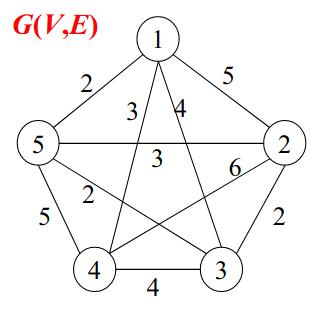
\includegraphics[scale = 0.4]{img/ch1.jpg}
  \end{figure}
  Procediamo con lo step 1, ottenendo $T$:
  \begin{figure}[H]
    \centering
    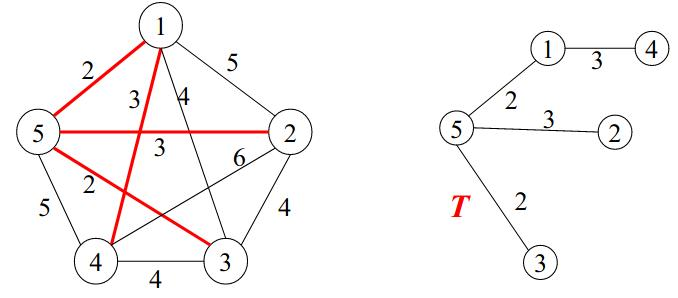
\includegraphics[scale = 0.4]{img/ch2.jpg}
  \end{figure}
  Procediamo con lo step 2, raddoppiando ogni arco di $T$:
  \begin{figure}[H]
    \centering
    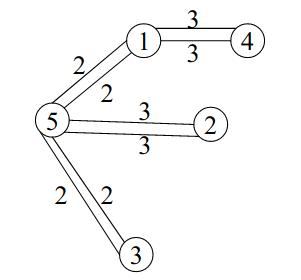
\includegraphics[scale = 0.4]{img/ch3.jpg}
  \end{figure}
  Procediamo con lo step 3, ottenendo $\epsilon$:
  \begin{figure}[H]
    \centering
    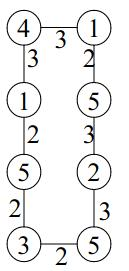
\includegraphics[scale = 0.4]{img/ch4.jpg}
  \end{figure}
  e con gli step 4 e 5 si ha:
  \begin{figure}[H]
    \centering
    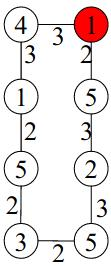
\includegraphics[scale = 0.4]{img/ch5.jpg}
  \end{figure}
  che deve essere ``letto'' in senso orario.\\
  Si ha quindi la sequenza di visita:
  \[\epsilon=\{1,5,2,5,3,5,1,4\}\]
  con la permutazione associata:
  \[\pi=\{1,5,2,3,4\}\]
  Si arriva quindi, con lo step 6, a:
  \begin{figure}[H]
    \centering
    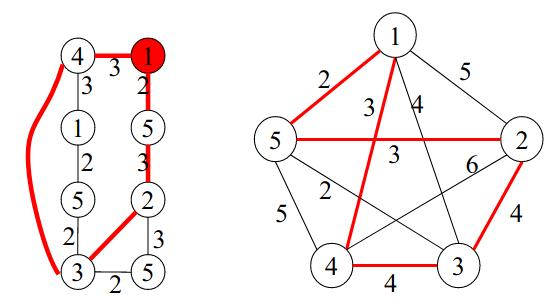
\includegraphics[scale = 0.4]{img/ch6.jpg}
  \end{figure}
  (avendo che comunque un arco tra due nodi che sostituisce un cammino tra quei
  nodi sicuramente costa meno o la più costa uguale, avendo la semimetrica)
\end{esempio}
L'\textbf{algoritmo di Christofides} trova quindi un'euristica cercando un
\textit{lower bound}, tramite l'albero di copertura.\\
\subsubsection{Cammino hamiltoniano e TSP}
Abbiamo visto che il cammino hamiltoniano è un problema \textbf{NP-complete} e
sappiamo che (si veda lezione nel capitolo sulle macchine di Turing,
cronologicamente fatta prima):
\[hamiltonianPath\leq_P TSP\]
(aggiungendo gli archi mancanti con costo maggiore dell'unità)
\begin{teorema}
  TSP (non metrico) non ha un'approssimazione costante a meno che $P=NP$.
\end{teorema}
\begin{proof}
  Sia $G=(V,E)$ il grafo in analisi su cui costruire il ciclo hamiltoniano.
  Costruiamo un
  $G'=(V', E', W)$ tale che:
  \[
    \begin{cases}
      w((u,v)) = 1\mbox{ sse } e=(u,v) \in E
      w(e)=\varepsilon\cdot|V|+1 \mbox{ altrimenti (pesando più di 1)}
    \end{cases}
  \]
  Si assume quindi  di avere un algoritmo $\varepsilon$-approssimato.
  Si hanno due casi:
  \begin{enumerate}
    \item l'algoritmo restituisce un tour di costo $|V|$ e quindi esiste il
    ciclo hamiltoniano
    \item l'algoritmo $A$ restituisce un tour con almeno un arco di costo
    $\varepsilon\cdot|V|+1$ e quindi $A(x)>\varepsilon\cdot |V|$
  \end{enumerate}
  Ma per definizione di $\varepsilon$-approssimazione ho che:
  \[\varepsilon\cdot opt(x)\geq A(x)\]
  e quindi si ha che:
  \[opt(x)>\frac{A(x)}{\varepsilon}>|V|\]
  cioèil tour ottimoèdi costomaggiore di $|V|$ e quindi non esiste un ciclo
  hamiltoniano (non c’è modo di avere Un tour di costo $|V|$).\\
  Pertanto $A$ diventa un algoritmo per deciderese esiste o meno un
  cammino hamiltoniano dove $A$ è polinomiale cioè è nella classe
  P. L’algoritmo è fatto come segue:
  \begin{itemize}
    \item se $A(x)=|V|$ allora ho che $opt(x)=|V|$ ed esiste il ciclo
    Hamiltoniano, altrimenti deve essere che $A(x)>\varepsilon\cdot |V|$ ma per
    costruzione ho che $opt(x)>|V|$ e quindi non esiste il ciclo hamiltoniano ma
    poiché il problema del ciclo hamiltoniano è in NP, ne consegue che P$=NP$,
    dimostrando il teorema.
  \end{itemize}
\end{proof}
Esistono quindi problemi che non hanno approssimazione costante.\\
Esistono anche problemi che hanno $\varepsilon$-approssimazione costante
$\forall\,\varepsilon$ piccolo a piacere (si parla di \textbf{Polynomial time
  approximation scheme (\textit{PTAS})}). 
\subsection{Closest string}
\textbf{Fatta velocemente e sembra fuori esame}.\\
In questo problema si ha in input una collezione di $k$ stringhe
$s_1,\ldots,s_k$ di lunghezza $l$. Si ha anche un input $d$ e in output si ha
una stringa $s$ tale che:
\[d_H(s,s_j)\leq d,\,\,\,\forall\,j= 1,\ldots,k\]
dove con $d_H(s,s')$ indichiamo la \textbf{distanza di Hamming} tra due stringhe
$s$ e $s'$, ovvero il numero di simboli diversi tra esse.
\begin{teorema}
  Closest string è risolvibile in tempo:
  \[O(d+1)^d|G|\]
  e se $d$ è piccolo, allora il tempo $O(d+1)^d$ è accettabile (esempio per
  distanza Hamming $d = 5$) anche quando l’input è molto grande  
\end{teorema}
\textbf{Dimostrazione extra su slide}.
\chapter{Macchina di Turing}
\section{Problemi intrattabili}
Trovare una soluzione polinomiale ad un algoritmo \textbf{NP-hard} come TSP
comporterebbe la rottura di tutte le chiavi crittografiche in quanto trovato un
algoritmo polinomiale per uno lo trovi per tutti.\\
Ci serve a questo punto una definizione più rigorosa di \textbf{algoritmo}, per
poterne calcolare meglio i tempi. Ricordiamo che per assunzione un algoritmo è
\textbf{efficiente} se è in tempo polinomiale rispetto alla dimensione
dell'input $x$, sapendo che $|x|=n$ (solitamente al più si arriva a $O(n^5)$ o
poco più poi si salta ad algoritmi esponenziali). Un algoritmo esponenziale è un
algoritmo \textbf{non efficiente}, il tempo cresce troppo velocemente
all'aumentare dell'input (anche se magari in alcuni casi non è in tempo
esponenziale). Si ricorda che si studia sempre il tempo nel 
\textbf{caso peggiore}, prenderemo quindi sempre l'O-grande sulla dimensione
dell'input $O(f(x))$.\\
Vediamo degli esempi:
\begin{itemize}
  \item un algoritmo che cerca l'arco minimo lavora in tempo polinomiale nel
  caso peggiore ed è quindi un \textbf{problema trattabile}
  \item problemi, come il test di primalità o TSP, che non hanno un algoritmo
  polinomiale sono \textbf{intrattabili}, infatti nessuno ha mai dimostrato che
  esiste un algoritmo efficiente
\end{itemize}
Tra i problemi intrattabili abbiamo però problemi che sono
\textbf{dimostrabilmente intrattabili}. Banalmente un problema che mi chiede di
stampare tutte le possibili sequenze per una certa proprietà è in questa
categoria, dovendo stampare tutte le sequenze possibili si ha $O(2^n)$ e si può
dimostrare che con meno operazioni non si stamperebbero alcune soluzioni
corrette.\\
Ci concentreremo su problemi intrattabili ma non \textit{dimostrabilmente
  intrattabili}.\\
Per anni problemi come il \textit{test di primalità} potevano garantire che
prima o poi si sarebbe trovato un algoritmo polinomiale (forse). Quindi abbiamo:
\begin{itemize}
  \item problemi dimostrabilmente intrattabili
  \item problemi non dimostrabilmente intrattabili, sono, diciamo, ``i più
  difficili'' tra i problemi intrattabili
  \item tutti gli altri problemi
\end{itemize}
\textbf{Un problema indecidibile non è un problema intrattabile}, in quanto non
si hanno proprio algoritmi che risolvono un certo problema e questo è
dimostrabile (c'è almeno un input che manda in crisi un algoritmo, che va in
loop infinito o sbaglia risposta) mentre un problema intrattabile comunque in
qualche modo lo posso risolvere ma in tempi troppo elevati.
\begin{shaded}
  L'algoritmo per il test di primalità funziona in $\log (n^{12})$, nella
  versione più efficiente sviluppata da un gruppo di indiani, che arriva ad
  ottenere un tempo polinomiale.
\end{shaded}
\section{Definizione della TM}
Definiamo quindi in modo più rigoroso il concetto di algoritmo per poter
dimostrare che un certo algoritmo può anche non esistere. Non ci basta più la
definizione di algoritmo come sequenza di passi logici, in quanto andrebbe anche
definito un certo linguaggio (con scelte, cicli, operazioni aritmetiche,
operazioni logiche) ma ancora non basterebbe, non si è ancora sicuri di poter
trasformare un certo input in un certo output (per qualunque problema in
input). Lo step mancante è la \textbf{macchina di Turing}, con essa si può
garantire quanto appena detto, con essa si formalizza il processo di calcolo,
ovvero la serie di passaggi che porta da un input ad un output. Turing ragionò
dicendo che normalmente si risolve un problema partendo da carta e penna,
ponendosi poi in un certo stato mentale in cui si risolve o si studia una parte
dell'input (ad esempio in uno stato \textit{leggi tutti} leggo ``step by step''
tutto l'input, senza cambiare sto mentale, che verrà cambiato quando finisco
quello precedente). Divide quindi l'input in \textit{caselle} su cui si fanno
operazioni semplici, spostandosi a destra o a sinistra di una casella, o
leggendo/scrivendo la casella corrente. Turing ipotizza di avere carta
illimitata. Quindi la MT avrà un nastro infinito che permette di memorizzare
informazioni e si ha una testina di lettura e scrittura. Si ha un meccanismo che
si pone in uno \textit{stato}, sulla base del contenuto letto dalla testina e
dallo stato posso scegliere di spostarmi di una testina a destra o di una a
sinistra, eventualmente dopo avere scritto e modificando, sempre eventualmente,
lo stato. Tutto questo basta per il \textbf{calcolo}, infatti:
\begin{teorema}[Tesi di Turing-Church]
  Non esiste nessun formalismo di calcolo che sia più
  potente della Macchina di Turing:
  \begin{center}
   ``Se un problema è umanamente calcolabile, allora esisterà una macchina di
    Turing in grado di risolverlo (cioè di calcolarlo)''
  \end{center}
  È una tesi che non ha dimostrazione formale (non avendo chiara la definizione
  di \textbf{calcolo}) ma è stata dimostrata
  empiricamente nel corso degli anni. Portando quindi a dire che il calcolo è
  ciò che può essere eseguito con un Macchina di Turing (anche se non tutti i
  meccanismi di calcolo sono equivalenti ad una TM, ad esempio gli automi a
  stati finiti).\\
  Quindi ciò che è computabile è computabile da una TM o da un suo equivalente
  (come un linguaggio di programmazione). Banalmente anche una rete neurale lo
  è. 
\end{teorema}
\begin{figure}
  \centering
  \begin{tikzpicture}
    \tikzstyle{every path}=[very thick]

    \edef\sizetape{0.7cm}
    \tikzstyle{tmtape}=[draw,minimum size=\sizetape]
    \tikzstyle{tmhead}=[arrow box,draw,minimum size=.5cm,arrow box
    arrows={east:.25cm, west:0.25cm}]
    \begin{scope}[start chain=1 going right,node distance=-0.15mm]
    \node [on chain=1,tmtape,draw=none] {$\ldots$};
    \node [on chain=1,tmtape] {};
    \node [on chain=1,tmtape] {$\triangleright$};
    \node [on chain=1,tmtape] (input) {b};
    \node [on chain=1,tmtape] {b};
    \node [on chain=1,tmtape] {a};
    \node [on chain=1,tmtape] {a};
    \node [on chain=1,tmtape] {a};
    \node [on chain=1,tmtape] {a};
    \node [on chain=1,tmtape] {$\sqcup$};
    \node [on chain=1,tmtape,draw=none] {$\ldots$};
    \node [on chain=1] {\textbf{Input/Output Tape}};
\end{scope}
  \end{tikzpicture}
  \caption{Esempio di nastro di una TM}
  \label{fig:tur}
\end{figure}
Formalizziamo quindi la macchina di Turing.
\begin{definizione}
  Si definisce formalmente una TM come la quintupla:
  \[TM=(K,\Sigma,k_0, \delta, F)\]
  \begin{itemize}
    \item insieme $K$ di stati
    \item un alfabeto $\Sigma$
    \item uno stato di partenza $k_0$
    \item una funzione di transizione $\delta$
    \item un insieme $F$ di stati finali
  \end{itemize}
  Si hanno inoltre i seguenti stati finali:
  \begin{itemize}
    \item $H$, per l'\textit{halt}
    \item $Y$, per lo \textit{yes}
    \item $N$, per il \textit{no}
  \end{itemize}
  Il simbolo $\sqcup$ specifica che non ho un simbolo e il simbolo
  $\triangleright$ mi specifica che da lì parte l'input.
\end{definizione}
\begin{definizione}
  La funzione di transizione esprime cosa fa passo-passo la TM:
  \[\delta:K\times\Sigma\to K\times \Sigma\times\{\leftarrow,\rightarrow,-\}\]
  Ovvero prende in input uno stato e un simbolo e può avere in input un cambio
  di stato oppure il cambio del simbolo in quel punto o lo spostamento della
  testina di una posizione (che può comunque restare ferma).\\
  Si possono avere diverse varianti di implementazioni, obbligando al testina a
  spostarsi (andando avanti e indietro per indicare che deve stare ferma
  etc$\ldots$).\\
  Vedremo poi che avere questa funzione di transazione comporta l'avere una
  \textbf{TM deterministica} e che si potrà sviluppare una \textbf{TM non
    deterministica}.
\end{definizione}
Ogni operazione sulla TM ha lo stesso tempo e quindi posso usare il numero di
passi per calcolare il tempo di risoluzione.\\
Per esprimere la computazione di una TM usiamo una \textbf{configurazione},
ovvero sulla base della definizione della TM e dello stato attuale devo
definire tutti i passi.
\begin{definizione}
  Un \textbf{configurazione} di una TM è definita da:
  \begin{itemize}
    \item lo stato in cui si trova
    \item la stringa sul nastro (definita da tutti i simboli a destra della
    testina e tutti quelli a sinistra, ai quali viene aggiunto quello sotto la
    testina)
    \item la posizione delle testina 
  \end{itemize}
  In base alla configurazione la TM saprà come procedere.\\
  La configurazione descrive in ogni istante lo stato della macchina e quindi si
  ha la seguente \textbf{configurazione iniziale}, per la stringa $X$ (che ha un
  carattere per posizione del nastro, al quale comunque viene aggiunto lo
  \textit{start} $triangleright$):
  \[(k_0,\triangleright X, 1)\]
  e ad un certo punto sia arriverà ad uno stato di arresto, per esempio dopo
  aver cambiato $X$ in $Y$ ed essere tornata nello stato 2:
  \[(H,\triangleright Y, 2)\]
  e quindi output sarà la stringa $Y$ (senza il $\triangleright$).\\
  Potrei avere anche $Y$ o $N$ al posto di $H$ in problemi decisionali, per
  capire magari se una certa stringa ha le caratteristiche desiderate o meno.
\end{definizione}
Vediamo alcuni esempi di costruzione di TM:
\begin{esempio}
  Si scriva la TM che calcoli il successore di un numero binario, che sarà
  l'input (e si da per scontato che sia correttamente formattato avendo solo 0 o
  1 come simboli). Si trascuri il riporto (nel senso che non aggiungo ulteriori
  bit).\\
  \begin{shaded}
    Vediamo nella pratica un esempio di somma binaria:\\
    prendo $01101010$ e sommo 1:
    \[10010101 \, +\]
    \[00000001=\]
    \[\rule{70pt}{.4pt}\]
    \[10010110\,\,\,\,\,\,\,\]
  \end{shaded}
  Definisco quindi la TM:
  \begin{itemize}
    \item $S=\{s_0,s_1\}$
    \item $\Sigma =\{\triangleright, \sqcup, 0,1\}$
    \item per la funzione di transizione si ha:
    \[\delta\to(s_0,[\triangleright, 0,1])\to(s_0,[\triangleright, 0,1],
      \rightarrow)\]
    \[\delta\to(s_0,\sqcup)\to(s_1,\sqcup,\leftarrow)\]
    \[\delta\to(s_1,0)\to(H,1,-)\]
    \[\delta\to(s_1,1)\to(s_1,0,\leftarrow)\]
    \[\delta\to(s_1,\triangleright)\to(H,\triangleright,-)\]

    ovvero scorro fino alla fine e inverto l'ultimo numero 
    (se è 0 diventa 1 e fine ma se è 1 lo rendo 0 e poi mi sposto a sinistra e
    se è un 1 diventa 0 e così via, fino alla
    fine dove metto 1, come prevede la somma binaria)
    \item $s_0$ è lo stato iniziale
  \end{itemize}
\end{esempio}
Volendo ad un certo punto si arriva allo stato finale $H$. In quel momento ho
una nuova stringa $Y$ (il risultato delle modifiche su $X$):
\[(H,\triangleright Y, -)\]
e la testina non deve più spostarsi. Questa può essere interpretata come uno
\textbf{stato di arresto}.\\
Un altro caso è avere una computazione infinita nel caso in cui, letto un
simbolo e lo stato, la testina ricopia il simbolo ma non si sposta ne a destra
ne a sinistra. Oppure una testina potrebbe ``rimbalzare'' infinitamente tra due
posizioni. Quest'ultima cosa può anche accadere tra molte posizioni, entrando
comunque in \textbf{loop infinito}, ritornando sempre, prima o poi, in una
configurazione (e si noti ``configurazione'', non coppia stato-simbolo) già
avuta. In questo caso la computazione è \textbf{non terminante} e la
computazione non produce alcun output. \textit{Quindi un insieme finito di
  elementi (stati, simboli e possibili transazioni) può comunque descrivere un
  comportamento infinito (infiniti passi)}.\\ 
Analizziamo meglio gli stati terminanti $Y$ e $N$ il primo indicante che la
stringa in input è accettata, avendo certe caratteristiche richieste, il secondo
che la stringa viene rifiutata. Non ho quindi più bisogno della stringa in
output, quindi posso lasciar scritto quello che voglio quando finisco, mi basta
sapere lo stato finale $Y$ e $N$.
\begin{esempio}
  Sistemiamo l'esempio precedente aggiungendo il riporto, dovendo aggiungere un
  bit. \\
 \textit{Si indica solo la funzione di transizione}.\\
  Scorro fino alla fine (quindi vado a destra indipendentemente dal simbolo fino
  ad un blank):
  \[\delta\to(s_0,[\triangleright, 0,1])\to(s_0,[\triangleright, 0,1],
    \rightarrow)\]
  Sono a destra dell'ultimo carattere di $X$ (avendo un blank):
  \[\delta\to(s_0,\sqcup)\to(s_1,\sqcup,\leftarrow)\]
  eseguo il conto tornando indietro:
  \[\delta\to(s_1,0)\to(H,1,-)\]
  \[\delta\to(s_1,1)\to(s_1,0,\leftarrow)\]
  sono tornato all'inizio:
  \[\delta\to(s_1,\triangleright)\to(s_2,1,\leftarrow)\]
  devo ``shiftare'' tutti i caratteri (per farlo semplicemente metto
  $\triangleright$ nel primo blank a sinistra del precedente $\triangleright$
  arrivando nello stato $s_2$, come indicato nello step precedente):
  \[\delta\to(s_2,\sqcup)\to(H,\triangleright,-)\]
  (avrei comunque potuto shiftare tutte le unità a destra di una posizione, o
  semplicemente, sapendo che ora sul nastro ho soli 0 dovrei tornare a destra di
  un passo, cambiare il primo 0 in 1 e aggiungere uno 0 in fondo alla
  stringa).
\end{esempio}
\begin{esempio}
  Vediamo un esempio in cui una TM riconosce una stringa binaria che è
  palindroma o meno.\\
  \textit{Si indica solo la funzione di transizione}.\\
  Se sono sullo start vado a destra di uno:
  \[\delta(s_0,\triangleright)\to (s_0,\triangleright, \rightarrow)\]
  se vedo 0 vado nello stato $zero$, scrivo $\sqcup$ e vado a destra:
  \[\delta(s_0,0)\to (zero,\sqcup, \rightarrow)\]
  analogo leggendo 1, andando nello stato $1$ scrivendo blank:
  \[\delta(s_0,1)\to (one,\sqcup, \rightarrow)\]
  vado in fondo alla stringa (qualsiasi incrocio tra gli stati $one$ e $zero $ e
  simboli 1 e 0 legga vado a destro riscrivendo lo stesso simbolo):
  \[\delta\to([zero, one],[0,1])\to(\delta\to([zero, one],[0,1],\rightarrow)\]
  sono in fondo alla stringa, se sono in stato $zero$ scrivo blank e torno
  indietro, in uno stato $zero'$:
  \[\delta(zero, \sqcup)\to(zero', \sqcup, \leftarrow)\]
  idem per stato $one$
  \[\delta(one, \sqcup)\to(one', \sqcup, \leftarrow)\]
  se sono in $zero'$ e leggo $0$ vado in stato $s_1$ e vado a sinistra: 
  \[\delta(zero', 0)\to(s_1,\sqcup, \leftarrow)\]
  se sono in $zero'$ e leggo $1$ la stringa non è palindroma, esco con stato
  $N$:
  \[\delta(zero', 1)\to(N,\sqcup, \leftarrow)\]
  idem per stato $one'$, andando in stato $s_2$:
  \[\delta(one', 1)\to(s_2,\sqcup, \leftarrow)\]
  \[\delta(one', 0)\to(N,\sqcup, \leftarrow)\]
  ora proseguo a sinistra fino ad un blank riscrivendo quanto letto:
  \[\delta(s_1,[0,1])\to(s_1,[0,1], \leftarrow)\]
  sono nel blank e torno allo stato iniziale, potendo ricominciare la
  computazione:
  \[\delta(s_1\sqcup)\to(s_0,\sqcup, \rightarrow)\]
  ma se la stringa (di cardinalità pari) è palindroma cancello tutto, devo
  quindi specificare che se in $s_0$ ho blank la stringa è valida:
  \[\delta(s_0,\sqcup)\to(Y, \sqcup,-)\]
  se invece la stringa è di cardinalità dispari, allo stato attuale, entra in
  loop, dobbiamo quindi aggiungere un uscita d:a $zero'$ o $one'$ in questo
  caso:
  \[\delta([zero',one'], \sqcup)\to(Y, \sqcup, -)\]
\end{esempio}
\begin{esempio}
  Scrivo una TM per decidere se la stringa in input è del tipo $a^nb^nc^n$.\\
  \textit{Si indica solo la funzione di transizione}.\\
  Se leggo $a$ vado nello stato $A$ e vado a destra
  \[\delta(s_0,a)\to (A,\sqcup, \rightarrow)\]
  Se leggo in $s_0$ $b$ o $c$ significa che non ho $a$ quindi esco:
  \[\delta(s_0,[b,c])\to (N,\sqcup, -)\]
  Se in $A$ trovo un'altra $a$ la lascio e vado a destra:
  \[\delta(A,a)\to (A,a', \rightarrow)\]
  Se in $A$ leggo $b$ vado in $B$, e vado a destra:
  \[\delta(A,b)\to (B,b', \rightarrow)\]
  se invece leggo $c$ non ho $b$ e esco:
  \[\delta(A,c)\to (N,\sqcup, -)\]
  se in $B$ e trovo $a$ non va bene:
  \[\delta(B,a)\to (N,\sqcup, -)\]
  Se in $B$ trovo un'altra $b$ la lascio e vado a destra:
  \[\delta(B,b)\to (B,b, \rightarrow)\]
  Se in $B$ leggo $c$ vado in $C$ e vado a sinistra a controllare:
  \[\delta(B,c)\to (C,c', \leftarrow)\]
  controllo tramite i sentinella indicati con $'$.\\
  Siamo in $C$ quindi:
  \[\delta(C,c')\to (C,c', \leftarrow)\]
  Se però vedo $b$ o $b'$ resto in $C$ e riscrivo:
  \[\delta(C,[b,b'])\to (C,[b,b'], \leftarrow)\]
  Per $A$ cambia, se vedo $a$ scorro:
  \[\delta(C,a)\to (C,a, \leftarrow)\]
  ma se vedo $a'$ torno in $s_0$:
  \[\delta(C,a')\to (s_0,a', \rightarrow)\]
  ma ora $A$ può incontrare $b'$, che va bene, o $c'$ che non va bene:
  \[\delta(A,b')\to (A,b', \rightarrow)\]
  \[\delta(A,c')\to (N,\sqcup, -)\]
  Per $C$:
  \[\delta(C,[b,c])\to (C,[b,c'], \rightarrow))\]
  Se sono in $s_0$ e trovo $a'$ ho finito le $a$:
  \[\delta(s_0,a')\to (s_0,a' , \rightarrow))\]
  idem:
  \[\delta(s_0,[b',c')\to (s_0,[b',c'] , \rightarrow))\]
  Vado in stato $check$ se:
  \[\delta(s_0,\sqcup)\to(check,\sqcup, \leftarrow)\]
  e proseguo fino a trovare solo $b'$ o $c'$, se trovo invece $b$ o $c$ esco.
  Diventa quindi molto lungo.
\end{esempio}
L'esempio sopra mostra quanto possa diventare lunga una semplice computazione
sulla TM, ci servirebbe quindi una sorta di \textit{TM alternativa}.
\begin{teorema}[teorema di B\"{o}hm-Jacopini]
  Qualunque algoritmo può essere implementato utilizzando tre sole strutture, la
  sequenza, la selezione e il ciclo, da applicare ricorsivamente alla
  composizione di istruzioni elementari
\end{teorema}
\begin{definizione}
  Si ha la \textbf{TM a $k$ nastri}, ovvero la \textbf{TM
    multi-nastro} dove ho $k$ nastri di lettura e scrittura, magari avendo
  l'input solo su un nastro o su multipli. La macchina quindi legge uno stato e
  $k$ simboli $\{\sigma_1\ldots,\sigma_k\}$. Prima dello spostamento quindi
  scrive tutti i simboli. Lo spostamento sarà uno per ogni nastro.
\end{definizione}
\begin{esempio}
  Risolviamo il precedente problema (decidere se la stringa in input è del tipo
  $a^nb^nc^n$) con $k$ nastri.\\
  Potrei usare 4 nastri, sul primo c'è l'input. Finché trovo $a$ scrivo sul
  primo, quando trovo $b$ passo a secondo e faccio lo stesso se leggo $c$. In
  ogni caso mi interrompo se dopo delle $b$ trovo $a$ o dopo $c$ trovo
  $a,b$. Infine torno indietro sui tre nastri e vedo se sono allineati.
\end{esempio}
Una \textbf{TM a $k$ nastri} non è più potente di una \textbf{TM a singolo
  nastro} (vale il rapporto linguaggio di programmazione e linguaggio
macchina). Esiste sempre una traduzione verso la TM a singolo nastro.\\
Per esempio invece un automa a stati finiti è meno potente di un TM, che può
spostarsi e scrivere dove vuole, a differenza degli automi.\\
Vediamo cosa quindi può fare una TM:
\begin{itemize}
  \item una TM può \textbf{computare} funzioni su stringhe
  \item una TM può \textbf{decidere} (rispondendo $Y$ o $N$) un linguaggio
  (ovvero un insieme finito o infinito di stringhe, come il caso sopra
  $a^nb^nc^n$), ovvero data una stringa in input è sempre in grado di dire se
  appartiene o meno al linguaggio. Un linguaggio è \textbf{decidibile}, o, più
  formalmente, \textbf{ricorsivo}, se esiste
  almeno una TM che decide il linguaggio, fermandosi sempre in $Y$ o
  $N$. Solitamente è un linguaggio finito, ma potrebbe anche essere infinito (ma
  tutte le stringhe sarebbero comunque riconoscibili)
  \item una TM può \textbf{accettare} un linguaggio, ovvero se fornisco una
  stringa in input che appartiene al linguaggio la riconosce come tale e prima o
  poi arriva allo stato $Y$, altrimenti la macchina potrebbe:
  \begin{itemize}
    \item fermarsi in uno stato $N$
    \item entrare in un loop infiniti, non avendo mai la risposta ma magari in
    realtà non è un loop infinito ma solo servono anni per avere la risposta
  \end{itemize}
  Quindi la TM non è in grado di distinguere completamente le stringhe che non
  fanno parte di un linguaggio. Un linguaggio è \textbf{linguaggio
    ricorsivamente enumerabile} è un linguaggio per cui data una stringa in
  input buona la TM si ferma, altrimenti la TM potrebbe o fermarsi o andare
  avanti all'infinito nella computazione. Posso enumerare tutte le stringhe che
  fanno parte del linguaggio, tramite una certa procedura. Potrei quindi avere
  un linguaggio infinito ma con 
  stringhe che mandano in loop la TM, anche se comunque non sono in grado di
  capire se sono in un loop o se prima o poi la stringa data in input verrà
  riconosciuto. Ci sono linguaggi che si può dimostrare 
  essere ricorsivamente enumerabili (e alcuni che non sono nemmeno
  ricorsivamente enumerabili)
\end{itemize}
Ricordiamo comunque che esistono problemi irrisolvibili, dimostrati tali, come la
soluzione di \textit{equazioni Diofantee}.\\
I linguaggi possono essere quindi ricorsivi, ricorsivamente enumerabili o non
ricorsivamente enumerabili. Un linguaggio finito è ricorsivo.\\
Se ho l'alfabeto $\Sigma$, presa la *-chiusura
di $\Sigma$ (che quindi comprende la stringa vuota e tutte le stringhe che
posso ottenere concatenando uno o più simboli di $\Sigma$), ovvero $\sigma^*$,
la TM riconosce subito la stringa in input in quanto costruita per funzionare
su $\Sigma$, quindi il linguaggio è ricorsivo. Se prendo $\Sigma^+$, ovvero
$\Sigma^*$ senza $\varepsilon$, ho comunque un linguaggio ricorsivo per lo
stesso motivo, dovendo solo controllare in più se $s_0$ è $\sqcup$.
\begin{teorema}
  Preso un linguaggio $L$ costruito alfabeto $\Sigma$ si ha che
  se $L\subseteq\Sigma^*$ se $L$ è ricorsivo è anche ricorsivamente
  enumerabile.
  \begin{proof}
    Se $L$ è ricorsivo esiste una TM che riconosce se, data una stringa $x$,
    $x\in L$, rispondendo $Y$ e risponde $N$ se $x\not\in L$.\\
    Costruisco ora una TM $M'$ che se il linguaggio non è ricorsivo allora vado
    in loop, indicato con $\infty,\uparrow,\bot$. Quindi quando la macchina sta
    per andare in $N$ cambio $\delta$ per ottenere il loop, ottenendo una
    macchina che va in loop se $x\not\in L$, mentre riconosce con $Y$ se $x\in
    L$ e quindi $L$ è ricorsivamente enumerabile. 
  \end{proof}
\end{teorema}
\begin{teorema}
  $L$ è ricorsivo sse $L$ è ricorsivamente enumerabile e il complementare di
  $L$, $\overline{L}$ è ricorsivamente enumerabile.
\end{teorema}
\begin{proof}
  Rispetto alla dimostrazione precedente, che garantisce che se $L$ è ricorsivo
  allora è ricorsivamente enumerabile, devo definire, per il complementare, una
  TM che va in loop se $x\in L$, andando altrimenti in loop. Presa quindi una TM
  $M$ che decide $L$, definisco $M'$ che accetta $L$, che quindi è
  ricorsivamente enumerabile. Definisco ora $M''$ che restituisce $Y$ se $x\in
  \overline{L}$ ovvero $x\not\in L$ (e $\infty$ se $x\not\in \overline{L}$,
  ovvero $x\in L$). Quindi $M''$ fa la stessa cosa di $M$ ma quando $M$ sta
  per rispondere $Y$ faccio andare $M''$ in loop e se $M$ va in $N$ faccio
  andare $M''$ in $Y$, tutto tramite un cambio di $\delta$.
\end{proof}
\begin{teorema}
  Preso un linguaggio $L$, se è ricorsivamente enumerabile e lo è anche il
  complementare $\overline{L}$ allora $L$ è ricorsivo.
\end{teorema}
\begin{proof}
  Presa una TM $M'$, se questa risponde $Y$ allora $M$ risponde $Y$. Presa $M''$
  se questa risponde $Y$ allora $M$ risponde $N$. $M'$ e $M'$ accettano $L$ e
  $\overline{L}$ quindi non possono dire $Y$ contemporaneamente e non rispondono
  $N$, andando in loop. $M$ non va mai in loop perché $x\in L\lor x\not\in L$
  per cui prima o poi una tra $M'$ e $M''$ si ferma. Devo quindi simulare
  l'esecuzione delle due macchine, raggruppandole in una sola, appunto
  $M$. Posso usare 4 nastri (due per le macchine e due per gli input) oppure
  posso mettere le due $\delta$ delle due macchine nella stessa (facendo prima
  un'operazione di $m'$ e poi una di $M''$ e così via), fino a che non si arriva
  ad uno $Y$ e, segnando tramite un nastro le configurazioni di $M'$ e $M''$,
  posso capire se far uscire $M$ con $Y$ o $N$, in base a chi tra $M'$ e $M''$ è
  uscito con $Y$. 
\end{proof}
A noi interessano comunque i \textbf{problemi} ma i linguaggi sono comodi per
parlare di \textbf{intrattabilità}, legandosi bene ai \textbf{problemi di
  decisione}.
\begin{definizione}
  Un problema di decisione è un problema con solo due possibili risposte, $Y$ e
  $N$.\\
  I problemi di decisione sono restrizioni di problemi di ottimo, ai quali viene
  aggiunto un \textbf{bound}, cambiando la domanda in una richiesta di esistenza
  di un caso che soddisfi il bound nel problema di ottimo (ma comunque potrei
  non avere tempi polinomiali, anche se il problema decisionale è più facile di
  quello di ottimo).
\end{definizione}
\begin{teorema}
  Un problema di decisione è sempre più facile del corrisponde problema di
  ottimo.
\end{teorema}
Posso associare un problema di decisione allo studio di un linguaggio, avendo
essi la stessa risposta, $Y$ o $N$. Un problema di decisione ha quindi un
corrispondente linguaggio, con l'input del problema che ha una corrispondente
stringa (di cui bisogna studiare appartenenza ad un linguaggio).\\
\begin{esempio}
  Il problema \textbf{Hamiltonian cycle problem (\textit{HCP})} (esiste anche la
  variante non con il ciclo ma con il cammino: \textbf{Hamiltonian path problem
    (\textit{HPP})}).\\ 
  Dato un grafo non completo e non pesato ci si chiede se c'è un modo per
  partire da un nodo e tornarci dopo aver toccato tutti i vertici una e una sola
  volta.\\
  Questo problema è di decisione ed è risolvibile, ma è difficile da risolvere
  in termini temporali (restringersi ai problemi decisionali non sempre implica
  miglioramenti in termini di tempo). HCP si risolve solo in tempo esponenziale.
\end{esempio}
\begin{teorema}
  Se il problema di decisione non è risolvibile in modo efficiente sicuramente
  il problema di ottimo associato non è risolvibile in modo efficiente.
\end{teorema}
\begin{teorema}
  Preso $\pi$ problema di decisione. Posso passare da $\pi$ ad un linguaggio
  $L(\pi)$ attraverso uno \textbf{schema di codifica}, che prende in input
  un'istanza del problema è mette in output una stringa $x$ del linguaggio. Se
  istanza ha risposta $Y$ ho $cod(x)\in L$ (e se risponde $N$ ho $cod(x)\not\in
  L$, con $cod$ che indica una 
  \textbf{codifica}, ovvero una traduzione dell'istanza nel linguaggio.\\
\end{teorema}
Risolvere un problema di decisione vuole dire essere in grado di riconoscere o
meno le stringhe del corrispondente linguaggio.
\begin{esempio}
  Pensando a HCP ho:
  \[L_{HCP}=\{y\in \Sigma^*|\mbox{ che corrispondono ad un'istanza con risposta
      Y}\}\]
  Sapendo che HCP è risolvibile so che esiste una TM che risolve il problema e
  il grafo può essere tradotto in stringa, ad esempio tramite una matrice di
  adiacenza.\\
  HCP è risolvile sse il linguaggio associato è decidibile, e quindi ricorsivo.
\end{esempio}
\begin{teorema}
  Quindi un problema decisionale è risolvile sse il linguaggio associato è
  decidibile, e quindi ricorsivo.
\end{teorema}
\begin{definizione}
  Il tempo di esecuzione di una TM è il conto dei passi di esecuzione nel caso
  peggiore.
\end{definizione}
\newpage
\section{Problemi non risolvibili}
Ci serve, in primis, una nuova TM:
\begin{definizione}
  Definiamo la \textbf{Universal Turing Machine (\textit{UTM})} come una TM che
  non fa un compito specifico in base alla $\delta$ ma prende in input un'altra
  TM $M$, un separatore ``;'' e l'input $x$ di $M$ e da in output la stessa cosa
  che darebbe $M$ con input $x$:
  \[UTM(M;x)\to M(x)\]
  Quindi calcola quello che calcola qualunque altra TM.
\end{definizione}
La UTM è simile a quello che fa tramite un linguaggio di programmazione, dove si
da una sequenza di istruzioni e un input, ottenendo un output. Un calcolatore
moderno è quindi una sorta di UTM (con l'hdd che corrisponde al nastro
infinito, non avendo potenzialmente limite potendo aggiungere altri dischi).\\
Esistono le \textbf{Small UTM (\textit{SUTM})} che riusano gli stati per ridurre
lo spazio usato.\\
Stati e simboli sono mediamente numeri naturali, e gli spostamenti pure (con
magari degli stati particolari). Un moderno calcolatore infatti ragiona solo su
numeri per definire tutto, dagli stati ai simboli.\\
Normalmente si ha che $UTM(M;x)$ ha due nastri sul primo $(M;x)$ e sul secondo
la configurazione attuale di $(M;x)$. Quindi una TM può simularne un'altra
salvando le configurazioni. La UTM tramite la sua $\delta$ poi copia lo stato di
uscita di $M$, magari scrivendo su un terzo nastro l'output.\\
\textbf{Posso quindi costruire una TM (la UTM) che simuli un'altra TM}, quindi
si è in grado di scrivere un algoritmo che prende in input un altro programma
scritto nello stesso linguaggio, che fa le stesse cose, e quindi il primo
algoritmo, per esempio, può dare le risposte opposte.\\
Si ha quindi che esistono \textbf{linguaggi non ricorsivi}, ovvero esistono
\textbf{problemi non decidibili} (come i dieci problemi proposti da Hilbert ad
inizio novecento).\\
Si ha che le TM sono \textbf{enumerate} in quanto possono essere associate ai
numeri naturali.\\
Ci sono problemi che possono essere chiaramente descritti per i quali sappiamo
che non esiste alcun algoritmo in grado di risolverli (di risolverli
\textbf{sempre}, basta quindi anche solo un caso per cui non posso avere tale
algoritmo). \textbf{Un problema non decidibile non è un problema intrattabile},
che sarebbe risolvibile ma solo in tempo esponenziale.\\
Non si può comunque dimostrare a priori che non esista un certo algoritmo (?)
\subsection{Halting problem}
Turing riconosce da subito come interessante l'\textbf{halting problem}. Si
cerca un algoritmo che data una certa coppia $(M;x)$, TM/input, mi dica se
quella macchina arriva a termine computazione o entra in loop infinito.
\begin{definizione}
  Definisco formalmente l'\textbf{halting problem} con il linguaggio $H$:
  \[H=\{M;x|\,M(x)\neq\bot\}\]
  Quindi se la stringa fa parte del linguaggio $M$ termina, altrimenti no.
\end{definizione}
\begin{teorema}
  Si ottiene però che $H$ non è ricorsivo e quindi l'halting problem non è
  decidibile.
\end{teorema}
\begin{proof}
  \textbf{DIMOSTRAZIONE DA SISTEMARE!}\\
  Immaginiamo per assurdo che $H$ sia ricorsivo e quindi esiste una TM $M_H$ che
  prende in input $(M;x)$ e mi da sempre in output $M(x)$, ma così sto facendo
  la stessa cosa della UTM. Ma $M_H$ non fa quello che fa la UTM, infatti fa:
  \[
    \begin{cases}
      Y& \mbox{ se }M(x)\neq \bot\\
      N& \mbox{ se }M(x) = \bot
    \end{cases}
  \]
  Quindi fa qualcosa in più della UTM, perché se finisce in loop deve capire che
  è in loop infinito, interrompere e restituire $N$.\\
  Assumo che $H$ quindi è ricorsivo e quindi $M_H$ esiste, anche se magari non
  la so costruire. Se esiste $M_H$ deve esisterne un'altra, chiamata $D$, che
  presa in input solo $M$ produce:
  \[D(M)\to M_H(M;M)\]
  Dando in input alla TM la descrizione della TM stessa (che è comunque
  ragionevole). Significa che:
  \[M_H(M;M)=
    \begin{cases}
      Y& \mbox{ se }M(M)\neq \bot\\
      N& \mbox{ se }M(M)=\bot
    \end{cases}
  \]
  ma voglio una macchina $D$ per la quale i risultati siano invertiti (è questa
  la chiave della dimostrazione per assurdo):
  \[D(M)=
    \begin{cases}
      Y& \mbox{ se }M(M)\neq \bot\to\infty\\
      N& \mbox{ se }M(M)=\bot\to Y
    \end{cases}
  \]
  Quindi $D$ cambia $N$ in $Y$ e $Y$ in $\infty$, presa in input una macchina
  $M$.\\
  Provo quindi a dare in input a $D$ $D$ stessa, ottenendo o il loop o
  $Y$. Ipotizziamo di andare in stato $Y$, quindi:
  \[M_H(D;D)=N\]
  che ci dice se $D$ su input $D$ termine e quindi $M_H$, per la definizione di
  $M_H$ deve rispondere $N$, Ma $M_H$ risponde $N$ sse $D(D)$ deve andare in
  loop infinito. Siamo arrivati ad un assurdo avendo detto che $M_H(D;D)=N$
  accade sse $D(D)=Y$. \\
  Inoltre se ipotizziamo che $D(D)$ va in loop allora $M_H(D;D)=Y$ che implica
  che $D(D)$ termina la computazione, sempre per definizione. Ho ottenuto quindi
  un'altra contraddizione, confermando la prova per assurdo.
\end{proof}
Si è dimostrato quindi che anche problemi ben definiti possono non essere
decidibili, problemi come il definire il comportamento di un programma dato un
input. Il problema comunque non è una potenza limitata della TM ma un limite
intrinseco al problema stesso.
\begin{teorema}
  Il linguaggio $H$ è ricorsivamente enumerabile, ovvero il problema è
  \textbf{parzialmente decidibile}. La macchina quindi riconosce una macchina
  che termina, altrimenti non si sa.  
\end{teorema}
\begin{proof}
  Devo trovare una macchina che termina in $Y$ che riconosce una stringa
  appartenente al linguaggio $H$.\\
  Costruisco quindi una $M_H'$ che prende in input una TM generica col suo
  input e si ha che:
  \[M_H'(M;x)=
   \begin{cases}
     Y &\mbox{ se } M(x)\mbox{ termina}\\
     N/\infty &\mbox{ altrimenti}
    \end{cases}
  \]
  Quindi se non termina non si sa che succede, ma potrebbe anche essere sempre
  in loop.\\
  Pensando a UTM ho che:
  \[UTM(M;x)=
   \begin{cases}
     Y &\mbox{ se } M(x)=Y\mbox{ avendo }M_H'=Y\\
     N &\mbox{ se } M(x)=N\mbox{ avendo }M_H'=Y\\
     H &\mbox{ se } M(x)=H\mbox{ avendo }M_H'=Y\\
     \infty &\mbox{ se } M(x)=\infty\mbox{ avendo }M_H'=\infty\\
    \end{cases}
  \]
  Quindi $M_H'$ è una UTM con gli stati finali leggermente modificati (quindi
  non più una UTM), avendo
  solo $Y$ (se termina) e $\infty$ (altrimenti). Abbiamo quindi dimostrato che è
  \textbf{parzialmente decidibile}, avendo che la macchina da $Y$ se la
  computazione è terminante e va in loop altrimenti.
\end{proof}
Ho quindi problemi non decidibili che sono parzialmente decidibili. Esistono
anche problemi legati a linguaggi \textbf{non ricorsivamente enumerabili}, per
cui quindi non si può \textbf{mai} dare risposta. Si hanno quindi problemi
nemmeno parzialmente decidibili. Pensiamo alle coppie $(M;x)$ che non terminano.
\begin{teorema}
   Esistono linguaggi \textbf{non ricorsivamente enumerabili} avendo quindi
   problemi non decidibili.
\end{teorema}
\begin{proof}
  Basti pensare che se $L$ è ricorsivo sse $L$ è ricorsivamente
  enumerabile. Quindi, pensando all'halting problem, $L_H$ non è ricorsivo ma è
  è ricorsivamente enumerabile. Ma allora $\overline{L_H}$, il linguaggio
  complementare non è ricorsivamente enumerabile: 
  \[\overline{L_H}=\{M;x|M(x)=\bot)\]
\end{proof}
\subsection{Problemi decidibili}
Studiamo ora i problemi decidibili catalogandoli in base ai tempi, nei casi
peggiori. Si hanno: 
\begin{itemize}
  \item algoritmi in tempo polinomiale rispetto alla dimensione dell'input
  \item algoritmi in tempo esponenziale rispetto alla dimensione dell'input,
  sono dimostrabilmente intrattabili
\end{itemize}
Bisogna capire se un problema cade in queste due categorie.\\
Il tempo di esecuzione viene calcolato tramite il numero di passi della TM.
\begin{definizione}
  Definiamo $t_M(x)$ come il tempo di calcolo di un TM $M$ su input $x$. Non è
  un caso peggiore ma dipendente dal singolo input specifico. Il tempo di
  calcolo è il numero di passi che esegue $M$ su input $x$ per dare una
  risposta. Concentrandosi sui problemi di decisione decidibili avrò sempre $Y$
  o $N$ se $x$ fa parte o meno del linguaggio. Ci concentriamo solo sui
  linguaggi ricorsivi.
\end{definizione}
Non si usa comunque il numero di passi nella realtà ma si usa l'O-grande,
studiando il caso peggiore, il numero massimo di passi.
\begin{definizione}
  Definiamo $T_M(n)$ come la \textbf{funzione di complessità temporale} come:
  \[T_M(n)=\max\{t_m(x)|\,|x|=n\}\]
\end{definizione}
\begin{definizione}
  Definisco la classe $P$ in base alle TM. La \textbf{classe P} è definita come:
  \[P=\{L|\mbox{ L è deciso da una DTM in tempo polinomiale } O(p(n))\}\]
  Con DTM che indica una TM deterministica, in cui per ogni coppia stato/simbolo
  la macchina può fare una sola cosa (leggere/*scrivere/spostarsi di uno)m e con
  $p$ una certa funzione polinomiale.\\
  È quindi la classe di problemi che so risolvere velocemente.
\end{definizione}
\begin{definizione}
  Definiamo la classe \textbf{\textit{time(f(n))}} come la classe dei linguaggi
  decisi da una TM entro un tempo $f(n)$. Quindi \textbf{\textit{time(n)}} sono
  tutti quelli decisi in tempo lineare, ad esempio (ma potrei anche per un
  qualsiasi $n^k$).\\
  Quindi:
  \[P=\cup_{i\geq 0} time(n^i)\]
  Infatti $P$ è l'unione di tutte le classi \textit{time} con funzioni
  polinomiali. \\
  La maggior parte dei problemi non supera, per il tempo polinomiale, un
  esponente pari a 10 ($N^{10}$).
\end{definizione}
\begin{teorema}
  Se un problema è nella \textbf{classe P} allora è risolvibile in un
  \textbf{tempo efficiente}.
\end{teorema}
Devo anche definire lo \textbf{spazio}, oltre al \textbf{tempo}.\\
\begin{definizione}
  Definisco lo \textbf{spazio di calcolo} come:
  \[s_M(x)=\mbox{ numero di celle del nastro usate dalla TM $M$ con input $x$}\]
  \[\mbox{durante la computazione}\]
  Il calcolo non è semplice come per il tempo, avendo anche decrementi. Quindi
  più che ``celle usate'' studiamo le ``celle visitate''.
\end{definizione}
\begin{definizione}
  Definisco $S_M(n)$ come la \textbf{funzione di complessità spaziale}:
  \[S_M(n)=\max\{s_M(x)|\,|x|=n\}\]
\end{definizione}
Spazio e tempo sono legati per una TM.\\
Innanzitutto se una computazione dura $n$ passi (tempo) posso dire che al più ho
usato $n$ celle (spazio), perché magari in qualche passo la testina rimane ferma
ma nel caso peggiore si sposta sempre. Si ha quindi:
\[S_M(n)\leq T_M(n)+n\]
con $+n$ perché sul nastro abbiamo comunque l'input di lunghezza $n$ (anche se
potrebbe non essere letto dalla TM). In alcuni casi non viene nemmeno
considerato come spazio usato in quanto non cambia la risposta in merito agli
studi di tempo (a meno di studiare tempi inferiori al tempo lineare, dove in
caso si specifica a parte di avere un input che occupa spazio $n$).
\begin{teorema}
  Se il tempo è limitato allora lo spazio è limitato ma non vale l'opposto
  (potrei avere banalmente un loop tra poche celle, avendo l'uso limitato di
  poche celle per un tempo illimitato).
\end{teorema}
\begin{teorema}
  Se ho una TM $M$ che lavora in spazio finito e tempo infinito, esiste una TM
  $M'$ che fa la stessa cosa di $M$ in tempo limitato.\\
  Quindi se lo spazio è limitato allora il tempo è limitato.
\end{teorema}
\begin{proof}
  Infatti la macchina $M'$ può trovarsi in un numero finito di stati $K$ e
  avendo spazio limitato ho un numero limitato $S_M(n)$ di celle in cui si trova
  la testina. Ho anche un numero finito di simboli in alfabeto $\sigma$ e
  quindi: 
  \[S_{M'}(n)\leq|k|\cdot |S_M(n)|\cdot |\Sigma|^{|S_M(n)|}\]
  avendo che prima o poi ritorno a stati già visti quindi la macchina se supera
  la quantità appena definita capisce di essere in loop (questo perché si ha a
  che fare con insiemi limitati e quindi tale ragionamento non va bene per
  l'halting problem). Quindi $|k|\cdot |S_M(n)|\cdot |\Sigma|^{|S_M(n)|}$ è
  anche un limite temporale per la seconda macchina (\textbf{rivedere
    quest'ultima affermazione}).
\end{proof}
Quindi data una certa macchina che lavora in un certo spazio $S(n)$ posso
costruire una macchina equivalente che da la stessa risposta in tempo limitato
$T(n)$. Si ha che se ho un problema che si risolve in spazio polinomiale, per
la formula appena scritta avrò tempo esponenziale. Invece, al contrario, tempo
polinomiale comporta spazio polinomiale.
\subsection{NonDeterministic Turing Machine}
I problemi nella \textbf{classe EXP} sono ancora in studio per capire se sono
\textbf{dimostrabilmente intrattabili}. Per il loro studio
si usano le \textbf{NonDeterministic Turing Machine (NDTM)} che sono comunque
puramente teoriche, in quanto non si è in grado fisicamente di costruirle. Nella
DTM deterministica avevo una $\delta$ mentre nella NDTM ho:
\[\Delta\subseteq (k\times \Sigma)\times (k\times \Sigma \times\{\leftarrow,
  \rightarrow, -\})\]
Con $\Delta$, detta \textbf{relazione di transizione}, che non è una funzione
(come era $\delta$) ma una relazione.\\ 
Nella DTM dato uno stato potevo passare ad un solo stato tramite $\delta$,
passando di stato in stato fino ad uno stato finale. Era una sequenza di
transizioni. \\
Nella NDTM ho delle \textbf{scelte}, ovvero la computazione non è una sequenza
di computazioni ma un \textbf{albero di computazione}. Da ogni stato posso
passare a uno tra più stati, a seconda della \textit{scelta}, formando così un
albero. Il singolo passo di computazione non è univocamente definito. Ogni
singolo ramo comunque è equivalente al passo di computazione della DTM. Tramite
$\Delta$ definisco il passaggio tra stati.\\
Per capire se una stringa è accettata o meno dalla NDTM, visto che potrei andare
sia in $Y$ che in $N$ (che in $H$) a seconda della varie computazioni
dell'albero, si ha che:
\begin{definizione}
  Una stringa $x$ è \textbf{accettata} da una NDTM se esiste una computazione
  tale per cui:
  \[(s_0,x,1)\to(Y, z, \rho_G)\]
  quindi se almeno un ramo dell'albero di computazione che termina nello stato
  $Y$. Tutti gli altri rami possono fare quello che vogliono, anche restare in
  loop.\\
  Se non c'è almeno un ramo $Y$ non è accettata. Gli altri possono andare in
  loop o in uno stato $N$.
\end{definizione}
\begin{definizione}
  Un linguaggio $L$ è \textbf{accettato} da una NDTM $N$ se per tutte le
  stringhe che fanno parte del linguaggio esiste almeno una computazione che
  termina nello stato $Y$, ovvero esiste una computazione per cui:
  \[\forall x\in L\Rightarrow N(x)=Y\]
\end{definizione}
\begin{definizione}
  Un linguaggio $L$ è \textbf{deciso} da una NDTM $N$ se, qualora la stringa $x$
  appartenga il linguaggio, esiste \textbf{almeno una} computazione tale per
  cui: 
  \[x\in L\rightarrow N(x)=Y\]
  altrimenti, se $x$ non appartiene al linguaggio, per \textbf{tutte} le
  computazioni, si ha che: 
  \[x\not\in L \rightarrow N(x)=N\]
  Non devo quindi avere loop in questo caso, tutte devono dare $N$.
\end{definizione}
\begin{esempio}
  Si ha:
  \[L=\{a^nb^{2n}\}\cup\{a^{2n}b^n\}\]
  Studiamo una DTM che riconosca tale linguaggio. Dalle DTM controlla prima il
  primo formato senza cambiare i simboli. Se vede che le $a$ sono più delle $b$
  passo al secondo step, dopo aver riconvertito i simboli in $a$ e $b$. Dopo
  aver analizzato il secondo insieme restituisce $Y$ o $N$. Tale funzione di
  transazione non è scontata.\\
  Una NDTM potrebbe essere:
  \[(s_0,x,1)\]
  che va in
  \begin{itemize}
    \item $(s_1,x,1)$, da cui parte lo studio del primo insieme
    \item $(s_2,x,2)$, da cui parte lo studio del secondo insieme
  \end{itemize}
  Data una stringa che non fa parte di $L$ tutti i rami terminano con
  $N$. Altrimenti almeno un ramo porta a $Y$ a seconda dei tipi di stringa
  accettati, se appartengono al primo o al secondo insieme. \\
  La scelta del ramo non è definita formalmente, è solo una \textit{scelta}. La
  macchina sa il ramo da scegliere dopo aver analizzato la stringa iniziale.
\end{esempio}
\begin{teorema}
  Una NDTM non è ``più potente'' di una DTM in termini di capacità di
  riconoscimento di un linguaggio. Se ho una NDTM che accetta un linguaggio
  sicuramente ho una DTM che lo fa.
\end{teorema}
\begin{proof}
  La NDTM non viene simulata da una DTM procedendo per rami, concludendoli, ma
  si procede per singoli passi su ogni ramo (onde evitare di incappare
  prematuramente in loop). Si scende quindi per livelli simulando poi tutti i
  rami (dovendo però ``tornare indietro'' ogni volta per passare al ramo
  successivo). Quindi muovendomi tra i rami posso simulare tramite una DTM
  quanto fa una NDTM.
\end{proof}
Le NDTM sono ``più potenti'' in termini di tempo di computazione.
\begin{definizione}
  La NDTM $N$ decide il linguaggio $L$ in tempo $T(N)$ se:
  \begin{itemize}
    \item $N$ decide $L$
    \item $\forall\,x\in \Sigma^*$ se;
    \[(s_0,x,1)\to(s_G, z, \rho_G)\]
    in $M^k$ passi, avendo $k\leq F(N)$
  \end{itemize}
  Trovo quindi uno $Y$ in ogni caso in meno di $F(n)$ passi.\\
  Ho quindi un ramo che in almeno $k$ passi porta in $Y$, per ogni stringa
  accettata, se $L$ è accettato. 
  \textbf{Rivedere definizione}
\end{definizione}
Il problema diventa quindi trovare il ramo giusto. Nei problemi dimostrabilmente
esponenziali richiedono che il ramo $Y$ sia lunghissimo mentre ci sono altri
problemi per i quali tale ramo richiederebbe tempo polinomiale per arrivare a
$Y$ ma non si sa quale sia tale ramo da seguire, la soluzione diventa quindi
provarli tutti, arrivando a tempi esponenziali.\\
Ponendo il limite $F(n)$ posso studiare che ogni singolo ramo non superi $F(n)$
quindi la NTDM impiega il tempo richiesto da un solo ramo per decidere e
accettare, perché di passo in passo capisce su quale ramo non proseguire
(???).\\
un altro modo di vedere la NDTM è pensare che parallelamente si sposti in tutti
i livelli fino a cercare uno $Y$ e se non lo trova risponda $N$. Il tempo è
comunque in termini di livello dell'albero. La NDTM è una macchina
\textbf{massicciamente parallela}.\\
Quindi la NTDM, per quanto non più potente in termini di riconoscimento, lo è in
base al tempo, basandosi sui livelli dell'albero. 
Si parla di \textbf{guess\&check}, per il metodo che individua il ramo da
seguire e lo controlla, controllando lo stato $Y$.\\
Ci interessa quindi il tempo di verifica. Ci sono problemi difficili da
risolvere e facili da verificare e altri che sono pure difficili da
verificare.\\
La classe dei problemi facilmente verificabili di cui non si ha una facile
risoluzione altro non è che la \textbf{classe NP}, che sono problemi polinomiali
in modo non deterministico.
\begin{definizione}
  la \textbf{classe NP} corrisponde all'insieme di linguaggi $L$ che sono decisi
  da una NDTM in tempo polinomiale:
  \[F(n)=O(p(n))\]
\end{definizione}
Si ha un rapporto tra $P$ e $NP$.
\begin{teorema}
  Data una NDTM $N$ che decide $L$ in tempo $F(n)$ esiste una DTM $M$ che decide
  $L$ in tempo $O(d^{F(n)})$, dove $d$ è una caratteristica particolare della
  NDTM, ovvero il \textbf{grado massimo di divisione dell'albero di
    computazione} di $N$. 
\end{teorema}
\begin{proof}
  $M$ ha vari nastri:
  \begin{itemize}
    \item il primo contiene $N$
    \item il secondo simula $N$
    \item il terzo contiene un numero in base $d$, inizialmente $1$
  \end{itemize}
  La macchina fa un passo di simulazione di $N$, andando nel primo ramo ($d=1$)
  a sinistra. A questo punto:
  \begin{itemize}
    \item trova $Y$ e si ferma
    \item trova $N$ quindi va avanti
    \item trova un altro stato, incrementa $d$ e passa al ramo indicato da
    $d$
  \end{itemize}
  e così via. Nello step successivo farà due passi e non uno, per ogni
  ramo. Valutando quindi eventuali nuove ramificazioni per ogni ramo. \\
  Se $N$ arriva a $Y$ allora troverò certamente uno $Y$ per $M$. Se arriva a $N$
  dopo un po' tutti i rami terminano in $N$ ma devo verificare la cosa e a quel
  punto $M$ termina con $N$.\\
  La simulazione richiede $d$ passi per il primo livello, $d^2$ per il secondo,
  $d^i$ per l'i-simo livello. Mi fermo a $d^{F(N)}$, al livello $F(n)$ e quindi
  ho tempo: 
  \[O(d^{F(N)})\]
  \textbf{capire meglio}
\end{proof}
La NDTM è quindi più potente per i tempi, per quanto ne sappiamo infatti che se
la NTDM lavora in $F(n)$, quindi in tempo polinomiale, la DTM che la simula
lavora in $d^{F(n)}$, quindi in tempo esponenziale. Quindi la NDTM è ``più
veloce'', anche se non lo sappiamo con certezza.\\
Rispetto al rapporto tra $P$ e $NP$ possiamo dire che $P\subseteq NP$, in quanto
una NDTM è un caso generale della DTM (dove la relazione non ha mai scelte). Si
ha inoltre che: 
\begin{itemize}
  \item ci sono problemi che non sappiamo dire se sono in $P$ o meno ma sappiamo
  che sono in $NP$ (vedasi test di primalità). Ma questo non aiuta rispetto agli
  altri problemi
  \item ci sono problemi che sappiamo essere in $NP$ ma nessuno ha mai trovato
  la dimostrazione che sia in $P$
\end{itemize}
Capire qualcosa in merito ai problemi del secondo tipo potrebbe portare a $P=NP$
o $P\not\subseteq NP$. Questo è uno dei 10 problemi aperti della matematica ed è
il più importante per l'informatica teorica.\\
A questo conosciamo quindi $P$, $NP$, $EXP$ (poste in ordine di ``è contenuto
in''):
\[P\subseteq NP \subseteq EXP\]
Anche se $p\subseteq NP$ è al centro di studi.\\
Ordiniamo i problemi in base alla difficoltà in queste due classi, tramite le
\textbf{riduzioni polinomiali} tra problemi, che ipotizziamo solo di decisione
per praticità, $A\to B$. Cerco una procedura che per ogni istanza del problema
$A$ la trasforma in un'istanza per un problema diverso $B$. Quindi un'istanza di
$A$, $I_A$, ha due risposte, $Y$ o $N$, ma posso passare tramite una certa
$f:I_A\to I_B$ avendo poi $I_B$ tale che $B$ avrà risposte, uguali a quelle di
$A$, $Y$ o $N$. Dato l'input, una stringa, $x$ di $A$, ho che lo trasformo in
input per $B$ potendo dire se la stringa appartiene o meno al linguaggio
associato ad $A$, mascherando il passaggio a $B$. La cosa ha tempo pari alla
somma tra il tempo della trasformazione più quello dell'algoritmo $B$.\\
Vediamo, ad esempio, se possiamo risolvere il problema del ciclo hamiltoniano
usando TSP, entrambi decisionali. Partendo da un'istanza del grafo per il ciclo
hamiltoniano creo un'istanza con gli stessi vertici, aggiungo gli archi per
ottenere un grafo completo (visto che TSP ha un grafo completo mentre ciclo
hamiltoniano no). Aggiungo anche i pesi (TSP ha un grafo pesato mentre ciclo
hamiltoniano no), mettendo il peso a 1 per i vecchi archi
e $K$, con $k\neq 1$, a quelli appena aggiunti. Manca quindi
solo il bound, che è $B=|V|$ per il ciclo hamiltoniano che ipotizziamo con archi
solo pesati a $1$ ma quindi in TSP non posso usare quelli aggiunti in quanto
uscirei per forza dal bound se usassi uno degli archi aggiunti, basta $K=2$. Ho
un ciclo hamiltoniano sse $B=|V|$ anche con TSP, che avrà un giro con gli stessi
archi del ciclo hamiltoniano presente nel primo problema, posto che esista,
avendo che se TSP rende $Y$ sse $B=|V|$ allora avrò un ciclo hamiltoniano nel
problema iniziale, avendo $Y$ in risposta anche per questo. Ho quindi ridotto il
ciclo hamiltoniano a TSP, e possiamo dire che quest'ultimo è più difficile di
ciclo hamiltoniano. Per esempio vedere figura \ref{fig:htsp}
\begin{figure}
  \centering
  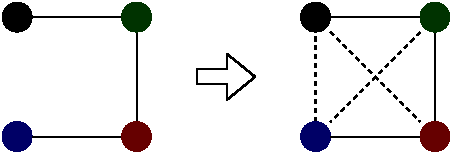
\includegraphics[scale = 0.9]{img/rid.pdf}
  \caption{Esempio di riduzione da ciclo hamiltoniano a TSP, con archi
    tratteggiati di peso 2 e archi normali di peso 1. Il colore dei vertici
    specifica che dalle due parti della trasformazione si ha lo stesso vertice}
  \label{fig:htsp}
\end{figure}
Controlliamo quindi i tempi. Voglio un costo della riduzione polinomiale e si ha
che l'aggiunta di archi, pesi e bound sono operazioni polinomiali.
\begin{definizione}
  Un problema $B$ è più difficile di un problema $A$, che ha in input la stringa
  $x$, sse:
  \[A\to B\]
  infatti ho:
  \[T(A(x))\leq F(x)+T(B(x))\]
\end{definizione}
\begin{definizione}
  Definiamo formalmente riduzione polinomiale tra un linguaggio $L_1$ e un
  linguaggio $L_2$ come:
  \[f:\Sigma_1^*\to \Sigma_2^*\]
  tale che:
  \[x\in L_1\iff f(x)\in L_2\]
  con $f$ calcolabile in tempo polinomiale ($O(|x|)$) dalla DTM. SI ha quindi
  che:
  \[L_1<_T L_2\]
\end{definizione}
\begin{teorema}
  Se si ha che $L_1<_T L_2$ e si ha che $L_2\in P$ allora sicuramente $L_1\in
  P$.\\
  Se avessi avuto $L_2\in NP$ o $L_2\not\in P$ non avrei informazioni su $L_1$. 

\end{teorema}
\begin{proof}
  Infatti e esiste un algoritmo polinomiale per $L_2$ allora, avendo una
  trasformazione polinomiale  ho che $f(x)+L_2$ è ancora polinomiale.
\end{proof}
\begin{teorema}
  Se si ha che $L_1<_T L_2$ e si ha che $L_1\not\in P$ allora ho che
  $L_2\not\in P$.
\end{teorema}
\begin{proof}
  Basta vedere ``al contrario'' il teorema precedente.
\end{proof}
Le riduzioni godono di proprietà:
\begin{itemize}
  \item riflessiva, $A\to A$
  \item transitiva, $A\to B\,\,\,\land \,\,\,B\to C\implies A\to C$, che essendo
  due trasformazioni in tempo polinomiale avrò comunque una trasformazione
  polinomiale 
\end{itemize}
Le riduzioni polinomiali \textbf{non sono sempre simmetriche} e quindi non sono
una relazione di equivalenza.\\
Abbiamo però una classe di equivalenza interna ai problemi NP, dove i problemi
contenuti sono i più difficili di NP e si riducono l'uno all'altro. Tali
problemi sono i problemi \textbf{NP-complete}.
\begin{definizione}
  Un linguaggio è \textbf{NP-complete} sse:
  \begin{itemize}
    \item $L\in NP$
    \item $L'<_TL,\forall\,L'\in NP$, tutti i linguaggi in NP si riducono a
    $L\in NP-complete$ e quindi i problemi in $NP-complete$ sono i più difficili
    di $NP$
  \end{itemize}
  Se ne risolvessi uno in tempo polinomiale risolverei tutti i problemi in NP in
  tempo polinomiale (ma ormai è assunto che non possa succedere anche se non si
  può dimostrare).
\end{definizione}
\begin{teorema}
  Ho che $P=NP$ sse esiste un linguaggio $L$ tale che:
  \[L\in NP-complete\cap P\]
\end{teorema}
\begin{proof}
  Se $P=NP$ allora sappiamo già che sarebbero polinomiali.\\
  Per l'altro verso ho che:
  \[\forall L'\in N, \,\,L<_T L\]
  e quindi esisterebbe un algoritmo polinomiale che risolve L per una DTM e
  quindi avrei un algoritmo polinomiale per ogni $L'\in NP$ per una DTM.
\end{proof}
Quindi se trovassi un algoritmo polinomiale per un NP-complete lo avrei per
tutti gli NP.
\begin{teorema}
  Se esiste un $L\in NP$ ma $L\not\in P$ allora:
  \[\forall L''\in \mbox{NP-complete}\]
  ho che $L''\not\in P$.
\end{teorema}
Dimostrando quindi che $P\neq NP$.\\
Andrebbe benissimo avere le prove di una di queste due situazioni, ma non esiste
ancora.\\
Per gli NP-complete vale anche la simmetria in quanto ogni problema NP-complete
è riducibile ad ogni altro problema NP-complete. Riprendendo l'esempio sopra so
che ciclo hamiltoniano è TSP, anche nelle forme decisionali, e quindi so che TSP
decisionale è NP-complete. La difficoltà è trovare almeno un problema
NP-complete, poi saprò che ogni altro a cui posso ridurlo è NP-complete.\\
Conosciamo moltissimi problemi NP-complete, molti riconosciuti tramite riduzioni
ma il primo è ottenuto tramite il \textbf{teorema di Cook}:
\begin{teorema}[teorema di Cook]
  SAT (che è stato già definito), che richiede un assegnamento di verità sulla
  formula $\phi$ in base all'assegnamento delle variabili $x_1,\ldots,x_n$, è
  NP-complete. 
\end{teorema}
\begin{proof}
  La dimostrazione completa è complessa ma vediamo qualche spunto.\\
  Si ha che SAT può essere risolto in tempo esponenziale, $O(2^n)$, provando
  tutti i possibili assegnamenti di verità possibili.\\
  Posso usare inoltre una NDTM che fa tutti i rami in parallelo, con ogni
  possibilità di assegnamento fatta in un ramo oppure posso dire che ``spara''
  un assegnamento a caso, che si suppone giusto, su un ramo e verifica che è
  giusto. In ogni caso con una NDTM avrei tempo polinomiale, $O(n\cdot m)$ per
  $n$ variabili e $m$ clausole.\\
  Per vedere che ogni problema NP, per semplicità decisionali, si riduce a SAT
  vedo che tutti i problemi in NP hanno in comune di avere un NDTM che li
  risolve in tempo polinomiale, che decide il linguaggio associato. Basta quindi
  dire che $\forall\Pi'\in NP$ ha associato una NDTM $N_\Pi'$ che lavora in
  tempo polinomiale e mi basta vedere che ogni NDTM che lavora in tempo
  polinomiale si può trasformare in una formula CNF, presa in ingresso da SAT,
  sfruttando poi gli stati finali della computazione di SAT. Se SAT dice che è
  soddisfacibile allora lo è il problema iniziale e quindi il problema è
  riducibile a SAT.
\end{proof}
SAT è stato il primo problema identificato come NP-complete ed è stato usato per
riconoscere gli altri problemi NP-complete.\\
La descrizione di una NDTM deve quindi corrispondere ad una $\phi$ di SAT per
far vedere che tutti i problemi NP si riducono a SAT. Si avrà una variabile per
ogni stato, una variabile per ogni carattere e una variabile per la posizione
della testina. Queste variabili saranno quelle che comporranno la $\phi$ e il
loro assegnamento comporterà la veridicità della formula.\\
Bisogna far vedere che $SAT<_T \Pi$ per far vedere che $\Pi$ è
NP-complete. Facendo poi vedere che un altro problema si riduce a $\Pi$ o SAT
dimostro che anche questo secondo problema è NP-complete. \\
Si ha che il problema del ciclo hamiltoniano e TSP, decisionali, siano
NP-complete.\\
Vediamo che $SAT<_T 3SAT$, che ha tre letterali in ogni clausola. Ho in input
una formula $\phi$ che deve diventare una $\phi_3$ tale che $\phi$ è
soddisfacibile sse $\phi_3$ lo è. La formula $\phi$ ha tante clausole in
congiunzione tra loro con un numero arbitrario di letterali ma $\phi_3$ deve
averne altrettante ma con soli tre letterali per clausola. Qualora si abbiano
clausole in $\phi$ con un solo letterale si aggiungono due letterali (che
indichiamo con $z$) in modo
però che la veridicità sia basata solo sulla variabile iniziale (questo vale per
tutte le trasformazioni che stiamo per mostrare, ovvero la veridicità deve
valere in base solo alle variabili iniziali della formula $\phi$). Tale clausola
che conteneva solo $x_1$ diventa una quadrupla clausola:
\[(x_1\lor z_1\lor z_2)\land (x_1\lor\neg z_1\lor z_2)\land (x_1\lor z_1\lor\neg
  z_2)\land(x_1\lor\neg z_1\lor\neg z_2)\] 
Se invece avessi una formula con due letterali diventa, aggiungendo una sola
variabile: 
\[(x_1\lor x_2\lor z_1)\land (x_1\lor x_2\lor \neg z_1)\]
Una formula a tre letterali resta ovviamente invariata mentre quelle a più
letterali vanno spezzate (aggiungendo poi variabili). Per esempio, avendo
quattro letterali, otterrei:
\[(x_1\lor x_2\lor z_1)\land (\neg z_1\lor x_3\lor z_2)\land (\neg z_2\lor
  x_4\lor z_3)\land\cdots\land(z_{n-3}\lor x_{n-1}\lor x_n)\]
Si vede che ogni formula di SAT può essere trasformata in una di 3SAT e quindi
anche quest'ultimo è NP-complete. Si dimostra che invece 2SAT non è NP-complete
ma ogni $K$SAT, con $K>2$, è NP-complete.\\
Anche, per esempio, il \textit{problema della colorabilità} è NP-complete, in
quanto può essere ridotto a SAT (non vedremo come).\\
Torniamo a parlare di TSP, non di decisione. Ho capito che serve tempo
esponenziale per risolverlo quindi si può pensare che sia NP-complete. Passo
quindi alla versione di decisione. Vedo però che ciclo
hamiltoniano, che è NP-complete, si riduce a TSP decisionale che quindi è
anch'esso NP-complete. Abbiamo comunque che TSP è più difficile del suo problema
decisionale, infatti D-TSP si riduce a TSP. Si ha quindi che TSP è
\textbf{NP-hard}, ovvero tutti i problemi NP si riducono ad esso ma il problema
stesso non è in NP (essendo un problema di ottimo e quindi non gli posso
associare un linguaggio) e quindi non è NP-complete (non essendo in NP). Per
TSP servirebbe una \textbf{macchina di Turing ad oracolo}.
\subsection{Rapporto spazio e tempo}
Aggiungiamo qualcosa a quanto già detto nelle sezioni precedenti.\\
\begin{definizione}
  Definisco la \textbf{funzione di complessità spaziale} come:
  \[f:\mathbb{N}\to\mathbb{N}\]
  con $f(n)$ che è il massimo numero di caselle utilizzate da una TM per
  decidere un certo linguaggio $L$ tutte le istanze di una certa dimensione,
  $n=|x|$. 
\end{definizione}
Sappiamo che, dal punto di vista del tempo (in notazione si ha $dtime=time$):
\[P=\bigcup_{k\geq 1}dtime(n^k)\]
\[NP=\bigcup_{k\geq 1}ntime(n^k)\]
\begin{definizione}
  Definiamo la \textbf{classe DSPACE} come l'insieme di tutti i linguaggi tali
  che sono decisi da una TM in spazio $O(f(n))$. Si ha che;
  \[PSPACE=\bigcup_{k\geq 1}dspace(n^k)\]
  avendo quindi limite polinomiale.
\end{definizione}
\begin{definizione}
  Definiamo la \textbf{classe NSPACE} come l'insieme di tutti i linguaggi tali
  che sono decisi da una NDTM in spazio $O(f(n))$. Si ha che:
  \[NPSPACE=\bigcup_{k\geq 1}nspace(n^k)\]
  avendo quindi limite polinomiale.
\end{definizione}
Come vale:
\[P\subseteq NP\]
Vale che:
\[PSPACE\subseteq NPSPACE\]
e per dimostrarlo mi concerto su una macchina che si preoccupa solo dello spazio
e non del tempo.\\
Prendiamo nuovamente il problema SAT e quindi ragioniamo sulla NDTM. Vediamo che
SAT è in NPSPACE per ovvi motivi (capisco che ramo scegliere e tale ramo ha una
casella per letterale, avendo spazio $n$) ma vediamo se appartiene anche a
PSPACE. Una DTM potrebbe provare tutte le possibilità in tempo esponenziale ma
in spazio polinomiale in quanto si sovrascrivono ad ogni tentativo le varie
caselle indicanti gli assegnamenti di verità ma la cardinalità di tali caselle è
sempre la stessa, una per ogni letterale, ovvero $n$. Quindi ho che $SAT\in
PSPACE$ anche se non è un'informazione così eclatante a causa del tempo
esponenziale.
\begin{teorema}[Teorema di Savitch]
  Si dimostra che:
  \[PSPACE=NSPACE\]
  Quindi la DTM e la NDTM hanno la stessa potenza dal punto di vista dello
  spazio di calcolo.
\end{teorema}
\begin{proof}
  Un problema abbiamo visto essere definito come \textbf{configurazione
    raggiungibile}, ovvero se una macchina può andare da una configurazione
  iniziale $c_i$ ad una finale $c_f$ in un certo numero di passi $t$, indicato
  con:
  \[(c_i,C_f,t)\]
  Prendo una
  configurazione intermedi $c_m$ e vedo se vale:
  \[\left(c_i,C_m,\frac{t}{2}\right)\land \left(c_m,C_f,\frac{t}{2}\right)\]
  Spezzo poi in modo D\&I di volta in volta, vedendo ricorsivamente se entrambi
  i rami sono validi.\\
  Vedo che lo stack delle chiamate ricorsive ha una certa profondità. Una NDTM
  andrebbe in spazio $f(n)$ ha associata una DTM che lavora in spazio
  $O(f^2(n))$ in quanto salvo le varie configurazioni dello stack ricorsivo,
  avendo $2^{\log f(n)}=f(n)$.\\
  (\textbf{rivedere tutta la dimostrazione, quanto scritto è errato in buona
    parte!})
  
\end{proof}
Abbiamo quindi $PSPACE=NPSPACE$ e che $P\subseteq NP$ quindi certamente:
\[P\subseteq PSPACE\]
\[NP\subseteq NPSPACE\]
Si ha quindi la figura \ref{fig:cla}.
\begin{figure}
  \centering
  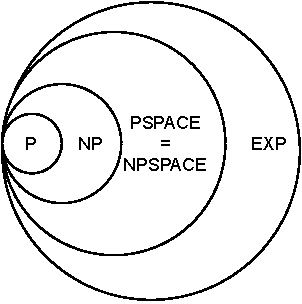
\includegraphics[scale = 0.9]{img/cla.pdf}
  \caption{Diagramma di Venn delle classi fin'ora descritte}
  \label{fig:cla}
\end{figure}
Abbiamo anche le classi $CO\_P$ e $CO\_NP$ ovvero le classi dei problemi
complementari $P$ e $NP$. Si ha che, a causa del determinismo:
\[CO\_P=P\]
ma quando si introduce il non determinismo le cose cambiano. La domanda iniziale
era del tipo \textit{esiste almeno uno} quindi il completamento è \textit{non
  esiste nessuno}, quindi devo verificare tutti i casi, andando in un caso che
nemmeno la NDTM riesce a risolvere, si finisce infatti nella classe
$EXP$. Quindi si ha che:
\[P\subseteq CP\_NP\land P\subseteq NP\]
non avendo un rapporto diretto e definito tra $NP$ e $CO\_NP$.




\chapter{Pattern matching}
Il \textbf{pattern matching} si occupa di ricercare un pattern $P$ in un testo
$T$. Si hanno:
\begin{itemize}
  \item \textbf{ricerca esatta}
  \item \textbf{ricerca approssimata}
\end{itemize}
\begin{definizione}
  Definiamo stringa come una sequenza di simboli appartenenti ad un dato
  alfabeto $\Sigma$, scritta come:
  \[X=x_1,\ldots,x_n,\,\,\,\forall x_i\in \Sigma\]
  ovviamente non è necessario che la stringa contenga tutti i simboli
  dell'alfabeto.\\
  Diamo alcune definizioni utili:
  \begin{itemize}
    \item $|X|$ indica la lunghezza della stringa
    \item $\varepsilon$ indica la stringa vuota
    \item $X[i]$ indica il carattere all'indice $i$ (partendo da 1 e non da 0)
    \item $X[i,j]$n indica la sottostringa che parte dall'indice $i$ e arriva
    all'indice $j$ (estremi inclusi). Inoltre se si hanno $i\neq j$ e $j\neq
    |X|$ si ha una \textbf{sottostringa propria}.\\
    (Esempio: per $X=bbaccbbaac$ ho la sottostringa $X[4,8]=ccbba$)
    \item $X[1,j]$ indico un \textbf{prefisso} (estremo finale incluso). Si ha
    inoltre il \textbf{prefisso proprio} se $j\neq |X|$ e si ha \textbf{prefisso
      nullo} se $j=0$ e si indica con $\varepsilon$.\\
    (Esempio: per $X=bbaccbbaac$ ho il prefisso $X[1,4]=bbac$)
    \item $X[i,|X|]$ indica un \textbf{suffisso} della stringa (estremi
    inclusi), di lunghezza $k=|X|-i+1$, avendo quindi il suffisso
    $X[|X|-k+1,|X|]$. Si ha inoltre che se ho $X[|X|,|X|+1]$ 
    allora ho il \textbf{suffisso nullo}, ovvero $\varepsilon$.\\
    (Esempio: per $X=bbaccbbaac$ ho il suffisso $X[8,10]=aac$ e il suffisso
    $X[11,10]=\varepsilon$)
    
\end{itemize} 
\end{definizione}
\begin{definizione}
  Definiamo il \textbf{pattern matching esatto} come la ricerca di tutte le
  occorrenze esatte di un pattern $P$ in un testo $T$.\\
  $P$ occorre esattamente in $T$, a partire dall'indice $i$ in $T$, sse:
  \[T[i,i+|P|-1]\mbox{ coincide con }P\]
  Quindi in output ho tutte le posizione $i$ nel testo tali per cui:
  \[T[i,i+m-1]\mbox{ coincide con }P\]
\end{definizione}
\begin{esempio}
  Dato il testo $T=bbaccbbaac$ e il pattern $P=ccbb$ ho un'occorrenza esatta a
  partire da $i=4$ nel testo.
\end{esempio}
L'algoritmo naive sarebbe quello di prendere una finestra $W$, di lunghezza $P$,
da far scorrere sul testo (avanzando ogni volta di un carattere). Ogni volta
tale finestra viene confrontata con $P$ confrontando tutti i caratteri e, in
caso di match, stampando in output l'indice di inizio della finestra sul
testo. Questo algoritmo è $O(|T|\cdot |P|)$ nel caso peggiore.\\ 
Questo algoritmo ignora le caratteristiche di testo e pattern, ignorando aspetti
che potrebbero accelerare la ricerca, trovabili tramite un'operazione di
preprocessamento.
\begin{definizione}
  Definiamo \textbf{distanza di edit} come il minimo numero di operazioni di
  sostituzione, cancellazione e inserimento di un unico simbolo per trasformare
  una stringa in un'altra (o viceversa). \\
  La distanza di edit tra due stringhe è simmetrica (anche se le operazioni
  saranno diverse il loro numero minimo sarà uguale).
\end{definizione}
\begin{esempio}
  Calcoliamo la distanza di edit tra $X_1=agtgcgt$ e $X_2=atgtgat$.\\
  Partiamo cancellando la $g$ in indice 2 di $X_1$:
  \[X_1=atgcgt\]
  \[X_2=atgtgat\]
  Inserisco quindi una ``a'' al penultimo indice di $X_1$:
  \[X_1=atgcgat\]
  \[X_2=atgtgat\]
  Infine sostituisco la ``c'' con una ``t'' all'indice 4 di $X_1$:
  \[X_1=atgtgat\]
  \[X_2=atgtgat\]
  Ho quindi una distanza di edit pari a 3.\\
  Per trasformare la seconda nella prima avrei dovuto inserire una ``g''
  all'indice 2 di $X_2$, cancellare la ``a'' al penultimo indice di $X_2$ e
  infine sostituire la ``t'' con una ``c'' al terzultimo indice di $X_2$. Si
  vede quindi come anche in questo caso avrei distanza di edit pari a 3.
\end{esempio}
\begin{definizione}
  Definiamo il \textbf{pattern matching approssimato} come la ricerca di
  occorrenze approssimate di un pattern $P$ in un testo $T$, con al più un certo
  errore $k$.\\
  Viene usata la \textnormal{distanza di edit}, che rappresenta l'errore che si
  commette nell'eguagliare una stringa con un altra.\\
  $P$ ha un'occorrenza approssimata in $T$, che finisce all'indice $i$, se
  esiste almeno una sottostringa $T[i-L+1,i]$ che ha distanza di edit con $P$ di
  al più $k$. $L$ è un certo valore non prevedibile in quanto sto ammettendo che
  il match sia su una stringa di lunghezza diversa da quella del
  pattern. Ovviamente in questo caso si possono avere più sottostringhe
  accettabili secondo i parametri richiesti.\\
  In output ho quindi tutte le posizioni $i$ di $T$ in cui finisce almeno una
  sottostringa che ha con $P$ distanza di edit al più uguale a $k$.
\end{definizione}
\begin{esempio}
  Prendiamo il testo $T=bbaccbbac$ e $P=ccbb$.\\
  Impongo $k=1$ e vedo che un match è ``ccbb'' terminante all'indice 6 del testo
  (avendo errore 1 massimo). Ovviamente ``ccbb'' terminante all'indice 7 va bene
  avendo errore nullo.\\
  
\end{esempio}
\begin{definizione}
  Definiamo \textbf{bordo} della stringa $X$, $B(X)$, che è il più lungo
  prefisso proprio che occorre come suffisso di $X$.
  \begin{esempio}
    Vediamo qualche esempio:
    \[X=baacagahabaac\implies B(X)=baac\]
    \[X=abababa\implies B(X)=ababa\]
    \[X=aaaaaa\implies B(X)=aaaaa\]
    \[X=aaaccbbaac\implies B(X)=\varepsilon\]
    \[X=aaaaaaaa\implies B(X)=aaaaaaa\]
  \end{esempio}
  Ovviamente può essere $\varepsilon$ (in primis se ho una stringa di lunghezza
  1).
\end{definizione}
\begin{definizione}
  Definiamo concatenazione tra una stringa $X$ e un simbolo $\sigma$ come:
  $X\sigma$
\end{definizione}
\begin{esempio}
  Dato $X=bba$ e $\sigma=d$ ho:
  \[X\sigma = bbad\]
\end{esempio}
\section{Pattern matching con automi}
Siamo nell'ambito del pattern matching esatto.\\
Ho un pattern di lunghezza $m$ e un testo di lunghezza $n$.\\
Abbiamo una fase di preprocessamento in tempo $O(m|\Sigma|)$ per calcolare la
funzione di transizione $\delta$.\\
Definiamo $\delta$ definita sul pattern $P$ come:
\[\delta:\{0,1,\ldots, m\}\times \Sigma\to\{0,\,\ldots, m\}\]
Quindi ad ogni coppia tra un simbolo e un intero tra 0 e $m$ corrisponde un
intero tra 0 e $m$. Nel dettaglio si hanno due casi:
\begin{enumerate}
  \item primo caso:
  \[\delta(j,\sigma)=j+1\iff j<m\land P[j+1]=\sigma\]

  \item secondo caso:
  \[\delta(j,\sigma)=k\iff P[j+1]\neq \sigma \lor j=m,\mbox{ con
    }k=|B(P[1,j]\sigma)|\]
  Con $k$ che è la lunghezza del bordo tra il prefisso corrente a cui viene
  concatenato il carattere $\sigma$. Si ha che $k\leq j$ per definizione (dato
  che sto calcolando il bordo su una stringa di lunghezza $j+1$). Con questa 
  transizione posso, eventualmente, andare ``indietro'' nel pattern ma comunque
  ``in avanti'' nell'automa.
\end{enumerate}
La transizione dallo stato $j$ allo stato $\delta(j,\sigma)$ avviene attraverso
il simbolo $\sigma$. Posso quindi passare allo stato $j+1$ o allo stato $k$.\\
Nell'automa avremo quindi gli archi etichettati coi simboli e i nodi
etichettati con gli indici da 0 a $m$.\\
Nella stringa gli indici partono comunque da 1 quindi l'indice 0 nelle formule
rappresenta una sorta di posizione prima dell'inizio della stringa. Qualora $k$
sia pari a 0 per la seconda formula mi sposto effettivamente in questo indice
posto prima della stringa (anche se avrò due stati diversi etichettati come 0
nell'automa).
\begin{esempio}
  Prendiamo il pattern:
  \[P=acacbabbaabac\]
  calcoliamo:
  \begin{itemize}
    \item $\delta(6,b)=7$ in quanto ho effettivamente $b$ come simbolo
    all'indice successivo a $6$, uso quindi la prima formula
    \begin{center}
      \begin{tikzpicture}[shorten >=1pt,node distance=2cm,on grid,auto]
        \node[state] (q_0) {$6$};
        \node[state] (q_1) [right=of q_0] {$7$};
        \path[->]
        (q_0) edge  node {b} (q_1);
      \end{tikzpicture}
    \end{center}
    \item $\delta(0,a)=1$, in quanto $a$ è il primo carattere, uso quindi la
    prima formula
     \begin{center}
      \begin{tikzpicture}[shorten >=1pt,node distance=2cm,on grid,auto]
        \node[state] (q_0) {$0$};
        \node[state] (q_1) [right=of q_0] {$1$};
        \path[->]
        (q_0) edge  node {a} (q_1);
      \end{tikzpicture}
    \end{center}
    \item $\delta(6,c)=2$ in quanto devo usare la seconda formula e avere:
    \[|B(P[1,6]c)|=|B(acacbac)|=|ac|=2\]
    \begin{center}
      \begin{tikzpicture}[shorten >=1pt,node distance=2cm,on grid,auto]
        \node[state] (q_0) {$6$};
        \node[state] (q_1) [right=of q_0] {$2$};
        \path[->]
        (q_0) edge  node {c} (q_1);
      \end{tikzpicture}
    \end{center}
    
    \item $\delta(0,c)=0$ in quanto devo usare la seconda formula e avere:
    \[|B(P[1,0]c)|=|B(c)|=|\varepsilon|=0\]
    \begin{center}
      \begin{tikzpicture}[shorten >=1pt,node distance=2cm,on grid,auto]
        \node[state] (q_0) {$0$};
        \node[state] (q_1) [right=of q_0] {$0$};
        \path[->]
        (q_0) edge  node {c} (q_1);
      \end{tikzpicture}
    \end{center}
    \item $\delta(13,a)=4$ in quanto devo usare la seconda formula e avere:
    \[|B(P[1,13]a)|=|B(acacbabbaabaca)|=|aca|=3\]
    \begin{center}
      \begin{tikzpicture}[shorten >=1pt,node distance=2cm,on grid,auto]
        \node[state] (q_0) {$13$};
        \node[state] (q_1) [right=of q_0] {$3$};
        \path[->]
        (q_0) edge  node {a} (q_1);
      \end{tikzpicture}
    \end{center}
  \end{itemize}
\end{esempio}
Facciamo due osservazioni:
\begin{enumerate}
  \item dallo stato 0 si arriva allo stato 0 per qualsiasi simbolo $\sigma\neq
  P[1]$ e quindi si arriva allo stato 1 attraverso $\sigma =P[1]$
  \item dallo stato $m$ si arriva sempre ad uno stato $k\leq m$ e da uno stato
  $m$ si può arrivare di nuovo ad uno stato $m$
\end{enumerate}
\begin{esempio}
  Se ho $P=aaaaaa$:
  \[\delta(6,a)=6\]
  in quanto:
  \[l=|B(aaaaaaa)|=|aaaaaa|=6\]
\end{esempio}
\begin{esempio}
  Sia dato un pattern $P=acacbac$, con $m=7$ e $\sigma=\{a,b,c\}$.\\
  Si hanno le seguenti transizioni $\delta(j,\sigma)$, calcolate solo sulla base
  delle formule.\\
  Parto con $\delta(j,\sigma)=j+1$:
  \begin{table}[H]
    \centering
    \begin{tabular}[H]{c||c|c|c}
      $j\backslash\sigma$ & a & b & c\\
      \hline
      \hline
      0 & 1 & & \\
      1 & & & 2\\
      2 & 3 & & \\
      3 & & & 4\\
      4 & & 5 & \\ 
      5 & 6 & & \\
      6 & & & 7\\
      7 & & &       
    \end{tabular}
  \end{table}
  Proseguo con $\delta(j,\sigma)=k$:
  \begin{table}[H]
    \centering
    \begin{tabular}[H]{c||c|c|c}
      $j\backslash\sigma$ & a & b & c\\
      \hline
      \hline
      0 & 1 & 0 & 0\\
      1 & 1 & 0 & 2\\
      2 & 3 & 0 & 0\\
      3 & 1 & 0 & 4\\
      4 & 3 & 5 & 0\\ 
      5 & 6 & 0 & 0\\
      6 & 1 & 0 & 7\\
      7 & 3 & 0 & 0      
    \end{tabular}
  \end{table}
\end{esempio}
In realtà algoritmo procede per induzione di riga in riga, riempendo la riga
basandosi con quella precedente, in $O(m|\Sigma|)$.\\
\newpage
\begin{esempio}
  Sia dato un pattern $P=acacbac$, con $m=7$ e $\sigma=\{a,b,c,d\}$.\\
  Aggiungo quindi un simbolo non appartenente al pattern, si ottiene:
   \begin{table}[H]
    \centering
    \begin{tabular}[H]{c||c|c|c|c}
      $j\backslash\sigma$ & a & b & c & d\\
      \hline
      \hline
      0 & 1 & 0 & 0 & 0\\
      1 & 1 & 0 & 2 & 0\\
      2 & 3 & 0 & 0 & 0\\
      3 & 1 & 0 & 4 & 0\\
      4 & 3 & 5 & 0 & 0\\ 
      5 & 6 & 0 & 0 & 0\\
      6 & 1 & 0 & 7 & 0\\
      7 & 3 & 0 & 0 & 0      
    \end{tabular}
  \end{table}
  Si aggiunge quindi una colonna di soli 0
\end{esempio}

\begin{esempio}
  Individuare un pattern sconosciuto di 6 caratteri e la tabella incompleta con
  solo $\delta(j,\sigma)=j+1$:
  \begin{table}[H]
    \centering
    \begin{tabular}[H]{c||c|c|c|c}
      $j\backslash\sigma$ & a & b & c & d\\
      \hline
      \hline
      0 & 1 &  &  & \\
      1 &  &  & 2 & \\
      2 &  & 3 &  & \\
      3 & 4 &  &  & \\
      4 & 5 &  &  & \\ 
      5 &  &  &  & 6\\
      6 &  &  &  &   
    \end{tabular}
  \end{table}
  Quindi banalmente il pattern è:
  \[P=acbaad\]
  Completo quindi la tabella con $\delta(j,\sigma)=k$:
  \begin{table}[H]
    \centering
    \begin{tabular}[H]{c||c|c|c|c}
      $j\backslash\sigma$ & a & b & c & d\\
      \hline
      \hline
      0 & 1 & 0 & 0 & 0\\
      1 &  1& 0 & 2 &0 \\
      2 &  1& 3 & 0 & 0\\
      3 & 4 & 0 & 0 & 0\\
      4 & 5 & 0 &2  &0 \\ 
      5 & 1 & 0 & 2 & 6\\
      6 & 1 & 0 & 0&  0 
    \end{tabular}
  \end{table}
\end{esempio}

\begin{esempio}
  Individuare un pattern sconosciuto di 6 caratteri e 3 simboli e la tabella
  incompleta:
  \begin{table}[H]
    \centering
    \begin{tabular}[H]{c||c|c|c|c}
      $j\backslash\sigma$ & a & b & c & d\\
      \hline
      \hline
      0 & 1 &  &  & \\
      1 & 2 &  &  & \\
      2 &  &  &  & \\
      3 &  &  &  & \\
      4 &  &  &  & \\ 
      5 &  &  &  & \\
      6 &  &  &  & 3  
    \end{tabular}
  \end{table}
  specifico i primi tre caratteri e gli ultimi due (il quarto non è
  ritrovabile).\\
  Quindi il pattern è:
  \[P=cac.ca\]
  per gli ultimi due sappiamo che avendo bordo 3 quindi gli ultimi due sono
  sicuro $ca$. Per le prime due uso la classica formula
  $\delta(j,\sigma)=j+1$. Per il terzo sfrutto l'ultima cella che ha segnato 3,
  che non è uno stato successivo ma ho il passaggio dallo stato 6 al 3 con c,
  implicando la lunghezza del bordo che calcolo sul pattern intero con $c$
  aggiunto è lungo 3 e quindi i primi tre simboli del pattern si ripetono negli
  ultimi 3 di questo pattern a cui è concatenato c. Quindi in 3 avrò c e in 5 e
  6 ca. Sul quarto carattere non posso dire nulla.
\end{esempio}

Vediamo quindi l'uso della funzione di transizione per trovare tutte le
occorrenze esatte nel testo. Si scandisce il testo per scandire il
testo. Ricordiamo che il preprocessamento (che non vedremo) ha tempo
$O(m|\Sigma|)$ mentre la scansione del testo ha tempo $O(n)$ in $T$.
Il procedimento è:
\begin{itemize}
  \item si parte dallo stato iniziale $s_0=0$
  \item il testo $T$ viene letto dalla posizione 1 alla $n$
  \item per ogni posizione $q$ da 1 a $n$ è associato uno stato $s_q$ ottenuto
  con la transizione dallo stato precedente $s_{q-1}$ tramite il simbolo $T[q]$:
  
\end{itemize}
\begin{center}
    \begin{tikzpicture}[shorten >=1pt,node distance=2cm,on grid,auto]
      \node[state] (q_0) {$s_0=0$};
      \node[state] (q_1) [right=of q_0]{$s_1$};
      \node[] (q_2) [right=of q_1]{$\cdots$};
      \node[state] (q_3) [right=of q_2]{$j$};
      \node[state, accepting] (q_4) [right=of q_3] {$s_q$};
      \node[] (q_5) [right=of q_4]{$\cdots$};
      \node[state] (q_6) [right=of q_5]{$s_n$};
      \path[->]
      (q_0) edge  node {T[1]} (q_1)
      (q_1) edge  node {T[2]} (q_2)
      (q_2) edge  node {T[q-1]} (q_3)
      (q_3) edge  node {T[q]} (q_4)
      (q_5) edge  node {T[n]} (q_6);
    \end{tikzpicture}
  \end{center}
Si hanno due supposizioni:
\begin{enumerate}
  \item si suppongache $j$ sia la lunghezza del più lungo prefisso di $P$ che ha
  un’occorrenza in $T$ che finisce in posizione $q-1$ (e che inizia quindi in
  posizione $q-j$)
  \item si supponga che $j$ sia lo stato $s_{q-1}$ a cui l'algoritmo arriva dopo
  aver letto il simbolo $T[q-1]$
\end{enumerate}
A questo si passa a $s_q=\delta(j,T[q])$. Il nuovo stato $s_q$ deve essere
calcolato. \\
Il calcolo di $s_q=\delta(j, T[q])$ si divide in due casi (anche se in realtà
poi sono tre):
\begin{enumerate}
  \item $j<m\,\,\,\land\,\,\,P[j+1]=T[Q]$, significa avere in $j+1$ lo stesso
  simbolo che ho appena letto:
  \begin{esempio}
    Si ha:
    \begin{table}[H]
      \centering
      \begin{tabular}{c||c|c|c|c|c|c|c|c|c|c|c|c|c|c|c|c|c}
        \hline
        & 1 & 2 & 3 & 4 & 5 & 6 & 7 & 8 & 9 & 10 & 11 & 12 & 13 &14&15&16&17\\
        \hline
        T=&a& a & a& b& a& c &c &a &b &a&c&c&c&a &c &b &a\\
        \hline
      \end{tabular}
    \end{table}
    matchando dal carattere 2 di T:
    \begin{table}[H]
      \centering
      \begin{tabular}{c||c|c|c|c|c|c|c|c}
        \hline
        & 1 & 2 & 3 & 4 & 5 & 6 & 7 &8\\
        \hline
        P=&a& b & a& c& c& a &b &. \\
        \hline
      \end{tabular}
    \end{table}

  \end{esempio}
  Il prefisso $P[1,j+1]$ (quindi quando ho $j+1=m$) si ha un'occorrenza di $T$
  che inizia in $q-(j+a)+1$, dopo aver letto il simbolo $T[q]$:
  \begin{center}
    \begin{tikzpicture}[shorten >=1pt,node distance=2.5cm,on grid,auto]
      \node[state] (q_0) {$j$};
      \node[state] (q_1) [right=of q_0] {$j+1$};
      \path[->]
      (q_0) edge  node {T[q]} (q_1);
    \end{tikzpicture}
  \end{center}
  Ho quindi che \textbf{il prefisso $P[1,m]=P$ ha un'occorrenza su $T$ che
    inizia in posizione $q-m+1$}:
  \begin{center}
    \begin{tikzpicture}[shorten >=1pt,node distance=2.5cm,on grid,auto]
      \node[state] (q_0) {$m-1$};
      \node[state] (q_1) [right=of q_0] {$m$};
      \path[->]
      (q_0) edge  node {T[q]} (q_1);
    \end{tikzpicture}
  \end{center}
  
  \item $j<m\,\,\,\lor\,\,\,P[j+1]\neq T[Q]$, che a sua volta si divide in:
  \begin{enumerate}
    \item $j<m\,\,\,\land\,\,\,P[j+1]\neq T[Q]$ ad esempio:
    \begin{esempio}
      Si ha:
      \begin{table}[H]
        \centering
        \begin{tabular}{c||c|c|c|c|c|c|c|c|c|c|c|c|c|c|c|c|c}
          \hline
          & 1 & 2 & 3 & 4 & 5 & 6 & 7 & 8 & 9 & 10 & 11 & 12 & 13 &14&15&16&17\\
          \hline
          T=&a& a & a& b& a& c &c &a &b &a&c&c&c&a &c &b &a\\
          \hline
        \end{tabular}
      \end{table}
      matchando dal carattere 2 di T:

      \begin{table}[H]
        \centering
        \begin{tabular}{c||c|c|c|c|c|c|c|c}
          \hline
          & 1 & 2 & 3 & 4 & 5 & 6 & 7 & 8\\
          \hline
          P=&a& b & a& c& c&a&c &. \\
          \hline
        \end{tabular}
      \end{table}
    \end{esempio}
    Si ha, con il bordo $k=B(P[1,j]T[q])$:
    \begin{center}
      \begin{tikzpicture}[shorten >=1pt,node distance=2.5cm,on grid,auto]
        \node[state] (q_0) {$j$};
        \node[state] (q_1) [right=of q_0] {$k$};
        \path[->]
        (q_0) edge  node {T[q]} (q_1);
      \end{tikzpicture}
    \end{center}
    Quindi \textbf{il prefisso $P[1,k]$ ha occorrenza su $T$ che inizia con il
      carattere $(q-k+1)$ del testo}. Faccio quindi un salto

    
    \item $j=m$, ad esempio:
    \begin{esempio}
      Si ha:
      \begin{table}[H]
        \centering
        \begin{tabular}{c||c|c|c|c|c|c|c|c|c|c|c|c|c|c|c|c|c}
          \hline
          & 1 & 2 & 3 & 4 & 5 & 6 & 7 & 8 & 9 & 10 & 11 & 12 & 13 &14&15&16&17\\
          \hline
          T=&a& a & a& b& a& c &c &a &b &a&c&c&c&a &c &b &a\\
          \hline
        \end{tabular}
      \end{table}
      matchando dal carattere 2 di T:
      \begin{table}[H]
        \centering
        \begin{tabular}{c||c|c|c|c|c|c|c|c}
          \hline
          & 1 & 2 & 3 & 4 & 5 & 6 & 7 &8\\
          \hline
          P=&a& b & a& c& c& a&b &a \\
          \hline
        \end{tabular}
      \end{table}
    \end{esempio}
    Ho quindi un'occorrenza di $P$ in $T$ che finisce in $q-1$. Il prefisso
    $P[1,k]$ ha occorrenza in $T$ che un'occorrenza che inizia in $q-m$ e una
    che inizia in $q-k+1$. Lo stato iniziale $m$ indica un’occorrenza di $P$ in
    $T$. Lo stato di arrivo $k$ è sicuramente minore o uguale a $m$. Se $k = m$,
    allora esiste una nuova occorrenza di $P$ in $T$ che risulta essere
    sovrapposta con la precedente di $m-1$ simboli. \textbf{Il prefisso
    $P[1,k]$ ha occorrenza in $T$ che un'occorrenza che inizia in $q-k+1$}
    

    \begin{center}
      \begin{tikzpicture}[shorten >=1pt,node distance=2.5cm,on grid,auto]
        \node[state] (q_0) {$j=m$};
        \node[state] (q_1) [right=of q_0] {$k$};
        \path[->]
        (q_0) edge  node {T[q]} (q_1);
      \end{tikzpicture}
    \end{center}
  \end{enumerate}
  Per rendere più semplice lo studio sono in grassetto i punti chiave dei tre
  casi. 
\end{enumerate}
Gli ultimi due casi possono essere riassunti con $j\geq m$ e $f\geq j$:
\begin{center}
  \begin{tikzpicture}[shorten >=1pt,node distance=2.5cm,on grid,auto]
    \node[state] (q_0) {$j$};
    \node[state] (q_1) [right=of q_0] {$f$};
    \path[->]
    (q_0) edge  node {T[q]} (q_1);
  \end{tikzpicture}
\end{center}
\textbf{Il prefisso di $P$ di lunghezza $f$ occorre in $T$ in posizione
  $q-f+1$ e se $f = m$, allora $P$ occorre in $T$ alla posizione $q-m+1$}.\\
In sostanza quindi l'algoritmo procede con tre step:
\begin{itemize}
  \item Si  parte dallo stato iniziale $s_0=0$  e si effettua una scansione di
  $T$ dal primo all’ultimo simbolo
  \item per ogni posizione $q$ di $T$ si effettua la transizione dallo stato
  corrente $s$ al nuovo stato $f = \delta(s,T[q])$ 
  \item ogni volta che il nuovo stato $f$ coincide con $m=|P|$, viene prodotta
  in output l’occorrenza $q-m+1$  
\end{itemize}
Avendo quindi lo pseudocodice:
\begin{algorithm}
  \begin{algorithmic}
    \Function{Scan-Text}{$\delta$, T, m}
    \State $n\gets|T|$
    \State $s\gets 0$
    \For {$q\gets 1$ to $n$}
    \State $f\gets \delta(s, T[q])$
    \If {$f==m$}
    \State \textbf{print} $q-m+1$
    \EndIf
    \State $s\gets f$
    \EndFor
    \EndFunction
  \end{algorithmic}
\end{algorithm}
Si ha quindi complessità lineare nella lunghezza del testo sia nel caso migliore
che peggiore.
\begin{esempio}
  Vediamo un esempio di scansione del testo dati:
  \begin{table}[H]
    \centering
    \begin{tabular}{c||c|c|c|c|c|c|c|c|c|c|c|c|c}
      \hline
      & 1 & 2 & 3 & 4 & 5 & 6 & 7 & 8 & 9 & 10 & 11 & 12 & 13 \\
      \hline
      T=&c& a & b& a& c& a &c &b &a &c&a&b&a\\
      \hline
    \end{tabular}
  \end{table}
  \begin{table}[H]
    \centering
    \begin{tabular}{c||c|c|c|c|c|c|c}
      \hline
      & 1 & 2 & 3 & 4 & 5 & 6 & 7 \\
      \hline
      P=&a& c & a& c& b& a &c \\
      \hline
    \end{tabular}
  \end{table}
  Sono dati, secondo la solita divisione:
  \begin{table}[H]
    \centering
    \begin{tabular}{c||c|c|c}
      $\delta(i,\sigma)$ & a & b & c\\
      \hline
      0 & 1 &  & \\
      1 &  &  & 2\\
      2 & 3 &  & \\
      3 &  &  & 4\\
      4 &  & 5 & \\
      5 & 6 &  & \\
      6 &  &  & 7\\
      7 &  &  & 
    \end{tabular}
  \end{table}
  \begin{table}[H]
    \centering
    \begin{tabular}{c||c|c|c}
      $\delta(i,\sigma)$ & a & b & c\\
      \hline
      0 & 1 & 0 & 0\\
      1 & 1 & 0 & 2\\
      2 & 3 & 0 & 0\\
      3 & 1 & 0 & 4\\
      4 & 3 & 5 & 0\\
      5 & 6 & 0 & 0\\
      6 & 1 & 0 & 7\\
      7 & 3 & 0 & 0
    \end{tabular}
  \end{table}
  inizio con solo lo stato iniziale:
  \begin{center}
    \begin{tikzpicture}[shorten >=1pt,node distance=2cm,on grid,auto]
      \node[state] (q_0) {$0$};
      \path[->]
      
      ;
    \end{tikzpicture}
  \end{center}

  leggo $c$ seguo la tabella e vado in $0$ da $0$:
  \begin{center}
    \begin{tikzpicture}[shorten >=1pt,node distance=2cm,on grid,auto]
      \node[state] (q_0) {$0$};
      \node[state] (q_1) [right=of q_0]{$0$};

      \path[->]
      (q_0) edge  node {c} (q_1)

      ;
    \end{tikzpicture}
  \end{center}
  leggo $a$ seguo la tabella e vado in $1$ da $0$:

\begin{center}
    \begin{tikzpicture}[shorten >=1pt,node distance=2cm,on grid,auto]
      \node[state] (q_0) {$0$};
      \node[state] (q_1) [right=of q_0]{$0$};
      \node[state] (q_2) [right=of q_1]{$1$};


      \path[->]
      (q_0) edge  node {c} (q_1)
      (q_1) edge  node {a} (q_2)

      ;
    \end{tikzpicture}
  \end{center}

  leggo $b$ seguo la tabella e vado in $0$ da $1$:

  \begin{center}
    \begin{tikzpicture}[shorten >=1pt,node distance=2cm,on grid,auto]
      \node[state] (q_0) {$0$};
      \node[state] (q_1) [right=of q_0]{$0$};
      \node[state] (q_2) [right=of q_1]{$1$};
      \node[state] (q_3) [right=of q_2]{$0$};

      \path[->]
      (q_0) edge  node {c} (q_1)
      (q_1) edge  node {a} (q_2)
      (q_2) edge  node {b} (q_3)

      ;
    \end{tikzpicture}
  \end{center}
  leggo $a$ seguo la tabella e vado in $1$ da $0$:

  \begin{center}
    \begin{tikzpicture}[shorten >=1pt,node distance=2cm,on grid,auto]
      \node[state] (q_0) {$0$};
      \node[state] (q_1) [right=of q_0]{$0$};
      \node[state] (q_2) [right=of q_1]{$1$};
      \node[state] (q_3) [right=of q_2]{$0$};
      \node[state] (q_4) [right=of q_3] {$1$};
     

      \path[->]
      (q_0) edge  node {c} (q_1)
      (q_1) edge  node {a} (q_2)
      (q_2) edge  node {b} (q_3)
      (q_3) edge  node {a} (q_4)
     
      ;
    \end{tikzpicture}
  \end{center}
  leggo $c$ seguo la tabella e vado in $2$ da $1$:

  \begin{center}
    \begin{tikzpicture}[shorten >=1pt,node distance=2cm,on grid,auto]
         \node[state] (q_0) {$0$};
        \node[state] (q_1) [right=of q_0]{$0$};
        \node[state] (q_2) [right=of q_1]{$1$};
        \node[state] (q_3) [right=of q_2]{$0$};
        \node[state] (q_4) [right=of q_3] {$1$};
        \node[state] (q_5) [below=of q_4] {$2$};
     

      \path[->]
      (q_0) edge  node {c} (q_1)
      (q_1) edge  node {a} (q_2)
      (q_2) edge  node {b} (q_3)
      (q_3) edge  node {a} (q_4)
      (q_4) edge  node {c} (q_5)
      
      ;
    \end{tikzpicture}
  \end{center}
  leggo $a$ seguo la tabella e vado in $3$ da $2$:


  \begin{center}
    \begin{tikzpicture}[shorten >=1pt,node distance=2cm,on grid,auto]
      \node[state] (q_0) {$0$};
        \node[state] (q_1) [right=of q_0]{$0$};
        \node[state] (q_2) [right=of q_1]{$1$};
        \node[state] (q_3) [right=of q_2]{$0$};
        \node[state] (q_4) [right=of q_3] {$1$};
        \node[state] (q_5) [below=of q_4] {$2$};
        \node[state] (q_6) [left=of q_5] {$3$};

      \path[->]
      (q_0) edge  node {c} (q_1)
      (q_1) edge  node {a} (q_2)
      (q_2) edge  node {b} (q_3)
      (q_3) edge  node {a} (q_4)
      (q_4) edge  node {c} (q_5)
      (q_5) edge  node {a} (q_6)
     
      ;
    \end{tikzpicture}
  \end{center}
    leggo $c$ seguo la tabella e vado in $4$ da $3$:

    \begin{center}
      \begin{tikzpicture}[shorten >=1pt,node distance=2cm,on grid,auto]
        \node[state] (q_0) {$0$};
        \node[state] (q_1) [right=of q_0]{$0$};
        \node[state] (q_2) [right=of q_1]{$1$};
        \node[state] (q_3) [right=of q_2]{$0$};
        \node[state] (q_4) [right=of q_3] {$1$};
        \node[state] (q_5) [below=of q_4] {$2$};
        \node[state] (q_6) [left=of q_5] {$3$};
        \node[state] (q_7) [left=of q_6] {$4$};


      \path[->]
      (q_0) edge  node {c} (q_1)
      (q_1) edge  node {a} (q_2)
      (q_2) edge  node {b} (q_3)
      (q_3) edge  node {a} (q_4)
      (q_4) edge  node {c} (q_5)
      (q_5) edge  node {a} (q_6)
      (q_6) edge  node {c} (q_7)

      ;
    \end{tikzpicture}
  \end{center}
    leggo $b$ seguo la tabella e vado in $5$ da $4$:

  \begin{center}
    \begin{tikzpicture}[shorten >=1pt,node distance=2cm,on grid,auto]
       \node[state] (q_0) {$0$};
      \node[state] (q_1) [right=of q_0]{$0$};
      \node[state] (q_2) [right=of q_1]{$1$};
      \node[state] (q_3) [right=of q_2]{$0$};
      \node[state] (q_4) [right=of q_3] {$1$};
      \node[state] (q_5) [below=of q_4] {$2$};
      \node[state] (q_6) [left=of q_5] {$3$};
      \node[state] (q_7) [left=of q_6] {$4$};
      \node[state] (q_8) [left=of q_7] {$5$};
     

      \path[->]
      (q_0) edge  node {c} (q_1)
      (q_1) edge  node {a} (q_2)
      (q_2) edge  node {b} (q_3)
      (q_3) edge  node {a} (q_4)
      (q_4) edge  node {c} (q_5)
      (q_5) edge  node {a} (q_6)
      (q_6) edge  node {c} (q_7)
      (q_7) edge  node {b} (q_8)
     
      ;
    \end{tikzpicture}
  \end{center}
  leggo $a$ seguo la tabella e vado in $6$ da $5$:

  \begin{center}
    \begin{tikzpicture}[shorten >=1pt,node distance=2cm,on grid,auto]
      \node[state] (q_0) {$0$};
      \node[state] (q_1) [right=of q_0]{$0$};
      \node[state] (q_2) [right=of q_1]{$1$};
      \node[state] (q_3) [right=of q_2]{$0$};
      \node[state] (q_4) [right=of q_3] {$1$};
      \node[state] (q_5) [below=of q_4] {$2$};
      \node[state] (q_6) [left=of q_5] {$3$};
      \node[state] (q_7) [left=of q_6] {$4$};
      \node[state] (q_8) [left=of q_7] {$5$};
      \node[state] (q_9) [left=of q_8] {$6$};
      

      \path[->]
      (q_0) edge  node {c} (q_1)
      (q_1) edge  node {a} (q_2)
      (q_2) edge  node {b} (q_3)
      (q_3) edge  node {a} (q_4)
      (q_4) edge  node {c} (q_5)
      (q_5) edge  node {a} (q_6)
      (q_6) edge  node {c} (q_7)
      (q_7) edge  node {b} (q_8)
      (q_8) edge  node {a} (q_9)
     
      ;
    \end{tikzpicture}
  \end{center}
    leggo $c$ seguo la tabella e vado in $7$ da $6$:

  \begin{center}
    \begin{tikzpicture}[shorten >=1pt,node distance=2cm,on grid,auto]
       \node[state] (q_0) {$0$};
      \node[state] (q_1) [right=of q_0]{$0$};
      \node[state] (q_2) [right=of q_1]{$1$};
      \node[state] (q_3) [right=of q_2]{$0$};
      \node[state] (q_4) [right=of q_3] {$1$};
      \node[state] (q_5) [below=of q_4] {$2$};
      \node[state] (q_6) [left=of q_5] {$3$};
      \node[state] (q_7) [left=of q_6] {$4$};
      \node[state] (q_8) [left=of q_7] {$5$};
      \node[state] (q_9) [left=of q_8] {$6$};
      \node[state] (q_10) [below=of q_9] {$7$};

      \path[->]
      (q_0) edge  node {c} (q_1)
      (q_1) edge  node {a} (q_2)
      (q_2) edge  node {b} (q_3)
      (q_3) edge  node {a} (q_4)
      (q_4) edge  node {c} (q_5)
      (q_5) edge  node {a} (q_6)
      (q_6) edge  node {c} (q_7)
      (q_7) edge  node {b} (q_8)
      (q_8) edge  node {a} (q_9)
      (q_9) edge  node {c} (q_10)
     
      ;
    \end{tikzpicture}
  \end{center}
  Essendo arrivati allo stato $m=7$, esiste un’occorrenzza di P in posizione
  $10-7+1 = 4 $.\\
  leggo $a$ seguo la tabella e vado in $3$ da $7$:

  \begin{center}
    \begin{tikzpicture}[shorten >=1pt,node distance=2cm,on grid,auto]
      \node[state] (q_0) {$0$};
      \node[state] (q_1) [right=of q_0]{$0$};
      \node[state] (q_2) [right=of q_1]{$1$};
      \node[state] (q_3) [right=of q_2]{$0$};
      \node[state] (q_4) [right=of q_3] {$1$};
      \node[state] (q_5) [below=of q_4] {$2$};
      \node[state] (q_6) [left=of q_5] {$3$};
      \node[state] (q_7) [left=of q_6] {$4$};
      \node[state] (q_8) [left=of q_7] {$5$};
      \node[state] (q_9) [left=of q_8] {$6$};
      \node[state] (q_10) [below=of q_9] {$7$};
      \node[state] (q_11) [right=of q_10] {$3$};

     

      \path[->]
      (q_0) edge  node {c} (q_1)
      (q_1) edge  node {a} (q_2)
      (q_2) edge  node {b} (q_3)
      (q_3) edge  node {a} (q_4)
      (q_4) edge  node {c} (q_5)
      (q_5) edge  node {a} (q_6)
      (q_6) edge  node {c} (q_7)
      (q_7) edge  node {b} (q_8)
      (q_8) edge  node {a} (q_9)
      (q_9) edge  node {c} (q_10)
      (q_10) edge  node {a} (q_11)
      
      ;
    \end{tikzpicture}
  \end{center}
  
  \newpage
  leggo $b$ seguo la tabella e vado in $0$ da $3$:

  \begin{center}
    \begin{tikzpicture}[shorten >=1pt,node distance=2cm,on grid,auto]
        \node[state] (q_0) {$0$};
      \node[state] (q_1) [right=of q_0]{$0$};
      \node[state] (q_2) [right=of q_1]{$1$};
      \node[state] (q_3) [right=of q_2]{$0$};
      \node[state] (q_4) [right=of q_3] {$1$};
      \node[state] (q_5) [below=of q_4] {$2$};
      \node[state] (q_6) [left=of q_5] {$3$};
      \node[state] (q_7) [left=of q_6] {$4$};
      \node[state] (q_8) [left=of q_7] {$5$};
      \node[state] (q_9) [left=of q_8] {$6$};
      \node[state] (q_10) [below=of q_9] {$7$};
      \node[state] (q_11) [right=of q_10] {$3$};
      \node[state] (q_12) [right=of q_11] {$0$};

      \path[->]
      (q_0) edge  node {c} (q_1)
      (q_1) edge  node {a} (q_2)
      (q_2) edge  node {b} (q_3)
      (q_3) edge  node {a} (q_4)
      (q_4) edge  node {c} (q_5)
      (q_5) edge  node {a} (q_6)
      (q_6) edge  node {c} (q_7)
      (q_7) edge  node {b} (q_8)
      (q_8) edge  node {a} (q_9)
      (q_9) edge  node {c} (q_10)
      (q_10) edge  node {a} (q_11)
      (q_11) edge  node {b} (q_12)

      ;
    \end{tikzpicture}
  \end{center}
    leggo $a$ seguo la tabella e vado in $1$ da $0$:

  \begin{center}
    \begin{tikzpicture}[shorten >=1pt,node distance=2cm,on grid,auto]
       \node[state] (q_0) {$0$};
      \node[state] (q_1) [right=of q_0]{$0$};
      \node[state] (q_2) [right=of q_1]{$1$};
      \node[state] (q_3) [right=of q_2]{$0$};
      \node[state] (q_4) [right=of q_3] {$1$};
      \node[state] (q_5) [below=of q_4] {$2$};
      \node[state] (q_6) [left=of q_5] {$3$};
      \node[state] (q_7) [left=of q_6] {$4$};
      \node[state] (q_8) [left=of q_7] {$5$};
      \node[state] (q_9) [left=of q_8] {$6$};
      \node[state] (q_10) [below=of q_9] {$7$};
      \node[state] (q_11) [right=of q_10] {$3$};
      \node[state] (q_12) [right=of q_11] {$0$};
      \node[state, accepting] (q_13) [right=of q_12] {$1$};

      \path[->]
      (q_0) edge  node {c} (q_1)
      (q_1) edge  node {a} (q_2)
      (q_2) edge  node {b} (q_3)
      (q_3) edge  node {a} (q_4)
      (q_4) edge  node {c} (q_5)
      (q_5) edge  node {a} (q_6)
      (q_6) edge  node {c} (q_7)
      (q_7) edge  node {b} (q_8)
      (q_8) edge  node {a} (q_9)
      (q_9) edge  node {c} (q_10)
      (q_10) edge  node {a} (q_11)
      (q_11) edge  node {b} (q_12)
      (q_12) edge  node {a} (q_13)
      ;
    \end{tikzpicture}
  \end{center}
  e mi fermo avendo concluso la scansione del testo. Ho trovato quindi solo una
  occorrenza che inizia all'indice 4.
\end{esempio}
\section{Algoritmo Knuth-Morris-Pratt}
Vediamo ora l'\textbf{algoritmo Knuth-Morris-Pratt (\textit{KMP})}.\\
Anche in questo caso si ha un preprocessing del pattern in tempo lineare alla
lunghezza del pattern $O(m)$. Si calcola una funzione di fallimento $\varphi$
per avere il preprocessamento. Si ha poi la scansione del testo in tempo $O(n)$.
\begin{definizione}
  Definiamo la funzione di fallimento, detta \textit{prefix function}
  $\varphi$: 
  \[\varphi:\{0,1, \ldots, \mathrm{m}\} \rightarrow\{-1,0,1, \ldots,
    \mathrm{m}-1\}\]
  tale che:
  \begin{itemize}
    \item $\varphi=|B(P[1,j])|$ se $1\leq j\leq m$
    \item $\varphi=-1$ se $j=0$
  \end{itemize}
\end{definizione}
\begin{esempio}
  Dato il pattern lungo 13:
  \begin{table}[H]
    \centering
    \begin{tabular}{c||c|c|c|c|c|c|c|c|c|c|c|c|c}
      \hline
      & 1 & 2 & 3 & 4 & 5 & 6 & 7 & 8 & 9 & 10 & 11 & 12 & 13 \\
      \hline
      P=&a& b & c& a& b& a &a &b &c &a&b&a&b\\
      \hline
    \end{tabular}
  \end{table}
  ottengo:
   \begin{table}[H]
    \centering
    \begin{tabular}{c||c|c|c|c|c|c|c|c|c|c|c|c|c}
      \hline
      & 1 & 2 & 3 & 4 & 5 & 6 & 7 & 8 & 9 & 10 & 11 & 12 & 13 \\
      \hline
      $\varphi$=&-1& 0 & 0& 0& 1 &2 &1 &1 &2&3&4&5&2\\
      \hline
    \end{tabular}
  \end{table}
\end{esempio}
Ci serve una definizione ricorsiva di bordo:
\begin{definizione}
  Si hanno 4 punti:
  \begin{enumerate}
    \item il bordo della stringa vuota è la stringa vuota stessa:
    \[B(\varepsilon)=\varepsilon\]
    \item il bordo di una stringa di un solo carattere è la stringa vuota:
    \[B(\sigma)=\varepsilon\]
    
    \item il bordo $B(X\sigma)$ della concatenazione tra una stringa $X$ e il
    simbolo $\sigma$ è:
    \[B(X\sigma)=B(X)\sigma\]
    \item il bordo $B(X\sigma)$ della concatenazione tra una stringa $X$ e il
    simbolo $\sigma$ è anche:
    \[B(X\sigma)= B(B(X)\sigma)\]
  \end{enumerate}
\end{definizione}
% aggiumngere esempio
\begin{definizione}
  Vediamo il calcolo di $\phi$ per induzione.\\
  I primi passi sono immediati:
  \[\phi(0)=-1\]
  \[\phi(1)=0\]
  Possiamo quindi calcolare $\phi(j)$ per $j>1$ supponendo che $\phi$ sia nota
  per tutti gli indici in $[0,j-1]$.\\
  Si ha:
  \[B(P[1,j])=B(P[1, j-1]P[j])\]
  e diciamo che:
  \[k_1=|B(P[1, j-1])|=\phi(j-1)\]
  Scriviamo anche:
  \[B(P[1,j-1]) = P[1,k_1]\]
  e chiamiamo:
  \[k_2=|B(P[1,k_1])|=\phi(k_1)=\phi(\phi(j-1))\]
  Si hanno due casi:
  \begin{enumerate}
    \item si ha $P[k_1+1]=P[j]$ quindi si ha:
    \[B(P[1,j])=B(P[1,j-1])P[j]\]
    Ne segue che:
    \[|B(P[1,j])| = |B(P[1,j-1])| + 1 \]
    Ma sappiamo che:
    \[|B(P[1,j])| = |B(P[1,j-1])| + 1 = k1 + 1 = \phi(j-1) + 1\]
    e quindi:
    \[|B(P[1,j])| = \phi(j-1) + 1\]
    e quindi possiamo dire che:
    \[\phi(j) = \phi(j-1) + 1 \]
    \item si ha $P[k_1+1]\neq P[j]$ quindi:
    \[B(P[1,j]) = B(B(P[1,j-1]) P[j])\]
    e sostituendo con $B(P[1,j-1]) = P[1,k_1]$:
    \[B(P[1,j]) = B(P[1,k_1] P[j])\]
    
  \end{enumerate}
  A questo punto dovrei separare due sottocasi per il secondo caso:
  \begin{enumerate}
    \item $P[k_2+1] = P[j]$
    \item $P[k_2+1] \neq P[j]$
  \end{enumerate}
  e andrei avanti ricorsivamente (su slide approfondimento anche su secondo
  livello di ricorsione).\\
  In generale possiamo dire che aggiungere un valore $k_p$ tale per cui:
  \[P[k_p+1]=P[j]\]
  implica che:
  \[\phi(j)=k_p+1\]
  mentre trovare tutti i valori $k_p$ tali per cui:
  \[P[k_p+1]\neq P[j]\]
  implica che a un certo punto si raggiunge un $k_p = -1$, che implica che il
  bordo 
  di $P[1,j]=0$ e quindi:
  \[\phi(j)=0=k_p+1\]
  Riassumo quindi la procedura:
  \begin{itemize}
    \item inizializzo $\phi(0)=-1$ e $\phi(1)=0$ e $j=2$ (per gli argomenti di
    $\phi$ che sono quindi maggiori di 1)
    \item setto $k=\phi(j-1)$
    \item divido nel due casi:
    \begin{enumerate}
      \item se $P[k+1] = P[j] $:
      \begin{itemize}
        \item setto $\phi(j)=k+1$
        \item $j=j+1$
      \end{itemize}
      e ricomincio
      \item se $P[k+1] \neq P[j] $:
      \begin{itemize}
        \item setto $k=\phi(k)$
        \begin{itemize}
          \item se $k=-1$ setto $\phi(j)=k+1$ e $j=j+1$ e ricomincio 
          \item altrimenti torno a testare i due casi
        \end{itemize}
      \end{itemize}
    \end{enumerate}
  \end{itemize}
  \newpage
  Possiamo quindi scrivere lo pseudocodice:
  \begin{algorithm}[H]
    \begin{algorithmic}
      \Function{Prefix}{$P$}
      \State $m\gets |P|$
      \State $\phi(0)\gets -1$
      \State $\phi(0)\gets 0$
      \For {$j\gets 2$ \textbf{to} $m$}
      \State $k\gets \phi(j-1)$
      \While {$k\geq 0\land P[k+1]\neq P[j]$}
      \State $k \gets \phi(k)$
      \EndWhile
      \State $\phi(j)\gets k+1$
      \EndFor
      \State \textbf{return} $\phi$
      \EndFunction
    \end{algorithmic}
  \end{algorithm}
  \textbf{su slide esempio di esecuzione}
\end{definizione}
Passiamo quindi alla scansione del testo.\\
La scansione del testo $T$ alla ricerca  di  $P$ avviene tramite una finestra
$W$ di confronto lunga m simboli che scorre lungo $T$ da sinistra a destra,
inizialmente posizionata in corrispondenza della posizione $i=1$ di $T$. Per
ogni posizione $i$ di $W$, ogni simbolo di $P$ viene confrontato con
il corrispondente simbolo in $W$, procedendo da sinistra a destra. Se
tutti i simboli sono confrontati con successo, allora nella posizione $i$ di $T$
esiste un’occorrenza di $P$. La finestra viene poi spostata verso destra in
una nuova posizione $j$ e si ripete il confronto.\\
La finestra viene spostata a destra utilizzando la funzione $\phi$. Il confronto
riparte dal simbolo del testo che aveva dato un mismatch con il pattern nella
precedente posizione di $W$, avendo quindi una scansione in $O(n)$.\\
Studiamo meglio lo spostamento di $W$.\\
Se ho $W$ in $i$ su $T$ e ho il primo carattere di $P$ che determina un mismatch
con $T$ in posizione $j>1$ ho che il simbolo di mismatch su $T$ è in
$i+j-1$. Per definizione sappiamo che $k=phi(j-1)$ è la lunghezza del bordo del
prefisso $P[1,j-1]$. Si ha quindi che:
\begin{itemize}
  \item $P[1,k]$ ha un’occorrenza su $T$ che inizia in posizione $i$
  \item $P[1,k]$ ha un’occorrenza su $T$ che inizia in posizione
  \[p=i+j-k-1=i+j-\phi(j-1)-1\]
\end{itemize}
Quindi il salto di $W$ da $i$ a $p$ garantisce di non perdere occorrenze di $P$
e garantisce che i primi $k$ simboli di $P$ hanno un matching con $T$ a partire
dalla nuova posizione $p$. Posso quindi far ripartire il contorno per la nuova
posizione $p$ di $W$ dalle posizioni:
\begin{itemize}
  \item $i+j-1$ su $T$
  \item $k+1$ su $P$
\end{itemize}
Sposto quindi $W$ a $p=i+j-\phi(j-1)-1$ e i primi $k=\phi(j-1)$ simboli di $P$
non vengono più confrontati con i corrispondenti simboli su $T$ nella nuova
posizione di $W$.\\
Si hanno dei casi particolari:
\begin{itemize}
  \item se $\phi(j-1)=0$ sposto $W$ a $p=i+j-1$ e i primi $k=0$ simboli di $P$
  non vengono più confrontati con i corrispondenti simboli su $T$ nella nuova
  posizione di $W$ quindi il confronto riparte da $i+j-1$ su $T$ e dal primo
  simbolo su $P$
  \item se $j=1$ sposto $W$ a $p=i+1$ e i primi $k=-1$ simboli di $P$
  non vengono più confrontati con i corrispondenti simboli su $T$ nella nuova
  posizione di $W$ quindi il confronto riparte da $i+1$ su $T$ e dal primo
  simbolo su $P$
  \item se $j=m+1$ sposto $W$ a $p=i+m-\phi(m)$ e i primi $k=\phi(m)$ simboli di
  $P$ 
  non vengono più confrontati con i corrispondenti simboli su $T$ nella nuova
  posizione di $W$ quindi il confronto riparte da $i+m$ su $T$ e dal 
  simbolo in posizione $\phi(m)+1$ su $P$
\end{itemize}

Questo algoritmo, tramite uno studia di complessità ammortizzata, nonostante il
doppio ciclo, ha complessità $O(n)$.\\
\textbf{Su slide esempio di esecuzione.}
\begin{algorithm}
  \begin{algorithmic}
    \Function{KMP}{$P, T,\phi$}
    \State $m\gets |P|$
    \State $n\gets |T|$
    \State $j\gets 0$
    \For {$q\gets 1$ \textbf{to} $n$}
    \While {$j\geq 0\land P[j+1]\neq T[1]$}
    \State $j \gets \phi(j)$
    \EndWhile
    \State $\phi(j)\gets j+1$
    \If {$j=m$}
    \State \textbf{return} $q-m+1$
    \EndIf
    \EndFor   
    \EndFunction
  \end{algorithmic}
  \caption{Algoritmo Knuth-Morris-Pratt}
\end{algorithm}
\section{Algoritmi shift-and}
\subsection{Algoritmo di Baeza-Yates e Gonnet}
Con questo algoritmo si ha il preprocessing del pattern $P$ di lunghezza $m$ in
tempo $O(|\Sigma|+m)$. Questo preprocessamento avviene tramite il calcolo di una
tabella $B$ di $|\Sigma|$ word di di bit $B_\sigma$, ognuna di lunghezza
$m$. Alla fine la scansione del testo $T$ di lunghezza $n$ è in $O(n)$.\\
Si sfrutta il paradigma \textbf{shift-and (esatto)} confrontando quindi delle
word binarie e non dei simboli.
\begin{definizione}
  L'operazione di \textbf{AND} definita su due word:
  \[w_1\mbox{ \textbf{AND} }w_2=w\]
  produce:
  \begin{itemize}
    \item $w[i]=1$ sse $w_1[i]\,\land w_2[i]=1$
    \item $w[i]=0$ altrimenti
  \end{itemize}
\end{definizione}
\begin{definizione}
  L'operazione di \textbf{or} definita su due word:
  \[w_1\mbox{ \textbf{or} }w_2=w\]
  produce:
  \begin{itemize}
    \item $w[i]=1$ sse $w_1[i]\,\lor w_2[i]=1$
    \item $w[i]=0$ altrimenti
  \end{itemize}
\end{definizione}
\begin{definizione}
  L'operazione di \textbf{RSHIFT} (shift a destra con MSB a 0) definita su una
  word: 
  \[\mathbf{RSHIFT}=w\]
  produce:
  \begin{itemize}
    \item $w[1]=0$
    \item $w[i]=w_1[i-1]$ con $2\leq i\leq |w|$
  \end{itemize}
  In pratica è lo spostamento dei bit di una posizione verso destra con bit più
  significativo a 0 (quindi visto che avrei il buco a sinistra lì metto 0).
\end{definizione}
\begin{definizione}
  L'operazione di \textbf{RSHIFT1} (shift a destra con MSB a 1) definita su una word:
  \[\mathbf{RSHIFT}=w\]
  produce:
  \begin{itemize}
    \item $w[1]=1$
    \item $w[i]=w_1[i-1]$ con $2\leq i\leq |w|$
  \end{itemize}
  In pratica è lo spostamento dei bit di una posizione verso destra con bit più
  significativo a 1 (quindi visto che avrei il buco a sinistra lì metto 1).
\end{definizione}
Si ha quindi che ogni word $B_\sigma$ è una word di $m$ bit $\{0,1\}$:
\[B_\sigma=b_1b_2,\ldots b_m\]
tale che:
\[b_i=B_\sigma[i]=1\iff P[i]=\sigma\]
\textbf{Esempio su slide.}\\
La tabella prodotta $B$ è quindi l'insieme delle word
$B_\sigma,\,\,\,\forall\,\sigma\in Sigma$
In pratica ho la tabelle con un numero di righe pari al numero di simboli. In
ogni riga ho una word dove a 1 ho solo gli elementi corrispondenti al carattere
della riga nel pattern (se $P=aba$ ho due righe: $B_a=101$ e $B_b=010$).\\
Si ha quindi il procedimento di calcolo:
\begin{enumerate}
  \item tutte le word di $B_\sigma$ sono inizializzate a bit di soli 0
  \item si inizializza una maschera $M$, che è una word di $m$ bit tutti uguali
  a 0 tranne il più significativo che è pari a 1
  \item si esegue una scansione di $P$ da sinistra verso destra, e per ogni
  posizione $i$ faccio:
  \begin{itemize}
    \item $B_{P[i]}=M\mbox{ \textbf{OR} }B_{P[i]}$
    \item $M=\mathbf{RSHIFT}(M)$
  \end{itemize}
\end{enumerate}
\begin{algorithm}
  \begin{algorithmic}
    \Function{Compute-B}{P}
    \State $m\gets |P|$
    \For {\textbf{every} $\sigma \in Sigma$}
    \State $B_\sigma \gets 00\ldots0$
    \EndFor
    \State $M \gets 10\ldots0$
    \For {$i\gets 1$ \textbf{to} $m$}
    \State $\sigma \gets P[i]$
    \State $B_\sigma \gets M\mbox{ \textbf{OR} }B_\sigma$
    \State $M=\mathbf{RSHIFT}(M)$
    \EndFor
    \State \textbf{return}
    \EndFunction
  \end{algorithmic}
  \caption{Algoritmo per il calcolo di $B$}
\end{algorithm}
Per la scansione del testo introduciamo la notazione:
\[P[1,i]=suff(T[1,j])\]
per indicare il prefisso lungo $i$ sul pattern $P$ occorre esattamente come il
suffisso di $T[1,j]$.
\begin{definizione}
  Dato un indice $j$, con $0\leq j\leq n$, con $n=|T|$, $D_j$ è una word di bit:
  \[D_J=d_1d_2\ldots d_m\]
  tale che:
  \[d_i=D_j[i]=1\iff P[1,i]=suff(T[1,j])\]
\end{definizione}
\begin{esempio}
  Preso:
  \[T=abcbcbcabaadc\]
  e:
  \[P=cbcbca\]
  Ottengo, ad esempio:
  \[D_7=101010\]
\end{esempio}
In pratica avanzo sul pattern è verifico se il prefisso mano a mano occorre come
suffisso nella prima parte del testo (parte definita da $j$ di $D_j$ che voglio
calcolare). Avanzando sul pattern se ho il prefisso coincide con quel suffisso
coincide metto 1, altrimenti 0 e poi aggiungo un carattere al prefisso avanzando
fino alla fine del pattern.\\
La word $D_0$ (ricordiamoci per l'indice inizia con 1 quindi è la word
relativa ad un indice prima di quello reale) è per definizione:
\[D_==00\ldots 0\]
poiché nessun prefisso di $P$ occorre come suffisso del prefisso nullo
$T[0,0]$.\\
La word $d_m=D_j[m]=1$ sse $P[1,m]=suff(T[1,j])$ quindi tutto il pattern ha
un'occorrenza che finisce in posizione $j$ sul testo $T$ e che inizia in
$j-m+1$.\\
Vediamo quindi come funziona la scansione del testo.\\
\begin{enumerate}
  \item si inizia dalla word $D_0=00\ldots0$
  \item per ogni valore di $j$ da 1 a $n=|T|$ calcolo $D_j$ a partire da
  $D_{j-1}$ che è stata calcolata al passo precedente
  \item ogni volta che $D_j$ ha l'ultimo bit uguale a $1$ ho in output $j-m+1$
  che è l'inizio dell'occorrenza di $P$ su $T$
\end{enumerate}
Bisogna capire come calcolare $D_j$ partendo da $j-1$:
\begin{itemize}
  \item se $i>1$:
  \[D_j[i]=1\iff P[1,i]=suff(T[1,j])\]
  ma questo può essere riscritto come:
  \[D_j[i]=1\iff P[1,i-1]=suff(T[1,j-1])\mbox{ \textbf{AND} }P[i]=T[j]\]
  ma la cosa può essere semplificata sapendo che $P[1,i-1]=suff(T[1,j-1])\iff
  D_{j-1}[i-1]=1$ e quindi posso dire che:
  \[D_j[i]=1\iff  D_{j-1}[i-1]=1\mbox{ \textbf{AND} }P[i]=T[j]\]
  ma sapendo che $P[i]=T[j]\iff B_{T[j]}[i]=1$ ho che:
  \[D_j[i]=1\iff  D_{j-1}[i-1]=1\mbox{ \textbf{AND} }B_{T[j]}[i]=1\]
  Avendo un calcolo basato sulla logica, con verità a 1, possiamo anche
  riscrivere come:
  \[D_j[i]\iff  D_{j-1}[i-1]\mbox{ \textbf{AND} }B_{T[j]}[i]\]
  e quindi:
  \[D_j[i]=  D_{j-1}[i-1]\mbox{ \textbf{AND} }B_{T[j]}[i]\]
  Si ha quindi che l'i-simo bit di $D_j$ è l'\textbf{AND} logico tra
  l'(i-1)-esimo bit di $D_{j-1}$ e l'i-esimo bit di $B_\sigma$ in corrispondenza
  di $\sigma=T[j]$
  
  \item se $i=1$:
  \[D_j[1]=1\iff P[1,1]=suff(T[1,j])\]
  ma questo può essere arricchito come:
  \[D_j[1]=1\iff P[1,1]= suff(T[1,j])\iff P[1]=T[j]\]
  e quindi posso dire, aggiungendo in \textbf{AND} un 1 che non cambia il
  risultato: 
  \[D_j[1]=1\iff P[1,1]= suff(T[1,j])\iff 1\mbox{ \textbf{AND} }P[1]=T[j]\]
  Quindi il risultato non cambia se si effettua l'\textbf{AND} logico con un bit
  uguale a 1 e quindi si ha:
  \[D_j[1]=1\iff 1\mbox{ \textbf{AND} }P[1]=T[j]\]
  ma si ha che $P[1]=T[j]\iff B_{T[j]}[1]=1$ e quindi:
  \[D_j[1]=1\iff 1\mbox{ \textbf{AND} }B_{T[j]}[1]=1\]
  e quindi:
  \[D_j[1]\iff 1\mbox{ \textbf{AND} }B_{T[j]}[1]\]
  che avendo logica booleana su bit diventa:
  \[D_j[1]= 1\mbox{ \textbf{AND} }B_{T[j]}[1]\]
  Quindi il primo bit della parola $D_j$ è uguale all'\textbf{AND} logico tra 1
  e il primo bit della parola $B_\sigma$ in corrispondenza del simbolo
  $\sigma=T[j]$  
\end{itemize}
\textbf{Esempio di calcolo su slide.}\\
Nell'esempio si arriva a dire che:
\[D_j=\mathbf{RSHIFT1}(D_{j-1})\mbox{ \textbf{AND} }B_{T[j]}\]
Posso quindi approfondire l'algoritmo di scansione:
\begin{enumerate}
  \item si inizializza una maschera del tipo $M=00\ldots 1$ (solo l'ultimo bit è
  pari a 1)
  \item si inizializza $D_0=00\ldots 0$
  \item per $j$ compreso tra 1 e $n$ calcolo:
  \[D_j=\mathbf{RSHIFT1}(D_{j-1})\mbox{ \textbf{AND} }B_{T[j]}\]
  \item ogni volta che $D_j\mbox{ \textbf{AND }M}$ è diverso da $00\ldots0$ ho
  in output la posizione $j-m+1$ di inizio occorrenza $P$ su $T$
\end{enumerate}
Avendo quindi nel complesso complessità:
\[O(|\Sigma|+m+n)\]
\textbf{Su slide due esempi, uno di esecuzione e uno di calcolo più mirato.}
\begin{algorithm}
  \begin{algorithmic}
    \Function{BYG}{P, T}
    \State $B\gets \mbox{Compute-B}(P)$
    \State $n\gets |T|$
    \State $D\gets 00\ldots 0$
    \State $M\gets 00\ldots 1$
    \For {$j\gets 1$ \textbf{to} $m$}
    \State $\sigma\gets T[j]$
    \State $D\gets \mathbf{RSHIFT}(D)\mbox{ \textbf{AND} }B_\sigma$
    \If{$D\mbox{ \textbf{AND} }M\neq 0$}
    \State \textbf{return} $j-m+1$
    \EndIf
    \EndFor
    \EndFunction
  \end{algorithmic}
  \caption{Algoritmo di Baeza-Yates e Gonnet}
\end{algorithm}
\subsection{Algoritmo di Wu e Manber}
Vediamo ora un algoritmo di \textbf{ricerca approssimata} con paradigma
\textbf{shift-and} (\textit{esempi per ogni step su slide}).\\
Dato un pattern $P$ e un testo $T$, su alfabeto $\Sigma$, e una soglia d'errore
$k$, si ha che $P$ ha un'occorrenza approssimata su $T$ in posizione finale $j$
se esiste una sottostringa $[j-L+1,j]$ che ha distanza di edit con il pattern di
al più $k$.\\
In merito all'algoritmo \textbf{Wu Manber (\textit{WM})}, implementato ad
esempio da \textit{grep}, si ha un preprocessing del pattern di lunghezza $m$ in
$O(|\Sigma| +m)$ tramite il calcolo di una matrice $B$ di $|\Sigma|$ parole di
$m$ bit. La scansione del testo per cercare le occorrenze approssimate è in
$O(nk)$. Il preprocessing è come in Baeza-Yates.\\
Studiamo la scansione.
L'algoritmo effettua $k+1$ scansioni per un indice $h$, tale che $0\leq h\leq
k$, dove la $h$-sima iterazione trova tutte le occorrenze del pattern con al più
$h$ errori. Con $h$ nullo ho le occorrenze esatte. La generica iterazione $h=k$
trova tutte le occorrenze in output all'algoritmo, ritrovando anche tutte le
soluzioni degli step precedenti di $h$. Sembra ci sia ridondanza di calcolo ma
si vedrà che si ha memorizzazione di tutte le occorrenze con un numero più basso
di $h$ rispetto a quello che si sta verificando. La generica iterazione $h$
calcola $n$ parole $D_J^h$ lunghe $m$ bit tali che $D_J^h[m]=1$ sse per ha
un'occorrenza approssimata che finisce in $j$ con al più $h$ errori (a conferma
che con $h=0$ ho lo shift-and esatto).\\
Si denoti con:
\[P[1,i]=suff_h(T[1,j])\]
il fatto che $P[1,i]$ occorre come suffisso di $T[1,j]$ \textbf{con al più $h$
  errori}. \\
Definiamo quindi, per un pattern $P$ lungo $m$:
\[D_j^h=d_1d_2\ldots d_m\,\,\,0\leq j\leq n,\,\,\, 0\leq h\leq k\]
tale che:
\[d_i=D_j^h[i]=1\iff P[1,j]=suff_h(T[1,j])\]
ricordando che $D_j^h$ è una parola di $m$ bit.\\
In particolare:
\begin{itemize}
  \item $D_0^h$ è per definizione $h$ bit più significativi pari a 1 e gli altri
  0, ovvero:
  \[
    \begin{cases}
      D_0^h=1&\mbox{ se } i\leq h \mbox{ (prime $h$ posizioni da sinistra)}\\
      D_0^h=1&\mbox{ se } i> h\mbox{ (ultime $m-h$ posizioni da destra)}\\
    \end{cases}
  \]
  infatti sui ha che:
  \[
    \begin{cases}
      \forall i\leq h, P[1,i]=suff_h(T[1,0])\\
      \forall i>h, P[1,i]\neq suff_h(T[1,0])
    \end{cases}
  \]
  Ne segue che $D_0^0$, avendo $h$ nullo, è per definizione $00\ldots 0$
  \item $d_m=D_j^h[m]=1\iff [1,m] = suff_k(T[1,j])$, avendo un'occorrenza che
  finisce in $j$ con al più $h$ errori e quindi con al più $k$ errori, avendo:
  \[D_J^h[m]=1\implies D_j^k[m]=1\]
  per cui non devo ogni volta ricalcolare
  \item $D_j^0$ corrisponde a Baeza-Yates
\end{itemize}
Nel dettaglio vediamo l'algoritmo:
\begin{itemize}
  \item alla prima iterazione $h=0$ $T$ viene scandito per $j$ da 1 a $n$ per
  calcolare tutte le word $D_j^0$ (ovvero Baeza-Yates)
  \item alla generica iterazione $h>0$ per ogni posizione $j$ del testo $T$
  viene calcolata $D_j^h$
  \item all'ultima iterazione $h=k$, ogni volta che la word $D_j^h$ calcolata ha
  il bit meno significativo pari a 1 viene prodotta in output la posizione $j$ di
  fine match con al più $k$ errori (non potrei sapere quella iniziale a causa
  degli errori) 
\end{itemize}
Bisogna quindi calcolare $D_j^h$ per qualsiasi $h>0$ e $j>0$, avendo che per
$h=0$ e $j=0$ ho word note.\\
Abbiamo che,per $i>1$:
\begin{itemize}
  \item ho un primo caso:
  \[D_j^h[i]=1\iff P[1,i]=suff_h(T[1,j])\impliedby P[1,i-1] =
    suff_h(T[1,j-1])\]\[\land P[i] = T[j] \]
  e quindi:
  \[D_j^h[i]=1\impliedby P[1,i-1] = suff_h(T[1,j-1])\land P[i] = T[j] \]
  Ma sappiamo che:
  \[[1,i-1] = suff_h(T[1,j-1])\iff D_{j-1}^h[i-1]=1\]
  e quindi posso riscrivere:
  \[D_j^h[i]=1\impliedby D_{j-1}^h[i-1]=1\land P[i] = T[j] \]
  ma so anche che:
  \[P[i]=T[j]\iff B_{T[j]}[i] = 1\]
  e quindi:
  \[D_j^h[i]=1\impliedby D_{j-1}^h[i-1]=1\land B_{T[j]}[i] = 1\]
  tolgo gli 1 per lo stesso ragionamento fatto con Baeza-Yates (avendoch a e
  fare con bit), ottenendo:
  \[D_j^h[i]\impliedby D_{j-1}^h[i-1]\land B_{T[j]}[i]\]
  implicazioni a sinistra $\impliedby$ non la posso togliere avendo altri casi
  \item ho un secondo caso:
   ho un primo caso:
  \[D_j^h[i]=1\iff P[1,i]=suff_h(T[1,j])\impliedby P[1,i-1] =
    suff_h(T[1,j-1]) \]
  avendo quindi un errore in meno nel primo caso e quindi $P[i]$ e $T[j]$
  possono essere diversi.\\
  Riduco:
  \[D_j^h[i]=1\impliedby P[1,i-1] = suff_h(T[1,j-1]) \]
  ma ho che:
  \[P[1,i-1] = suff_h(T[1,j-1]) \iff D_{j-1}^{h-1}[i-1]=1\]
  quindi:
  \[D_j^h[i]=1\impliedby D_{j-1}^{h-1}[i-1]=1 \]
  e quindi:
  \[D_j^h[i]\impliedby D_{j-1}^{h-1}[i-1] \]
  \item caso 3:
  \[D^h_j[i] = 1 \iff P[1,i] = suff_h(T[1,j])\impliedby P[1,i] =
    suff_{h-1}(T[1,j-1])\]
  e quindi $T[j]$ genera un errore.\\
  Compatto in:
  \[D^h_j[i] = 1 \impliedby P[1,i] =    suff_{h-1}(T[1,j-1])\]
  ma so che:
  \[ P[1,i] = suff_{h-1}(T[1,j-1])\iff  D_{j-1}^{h-1}[i]=1\]
  e quindi:
  \[D^h_j[i] = 1 \impliedby D_{j-1}^{h-1}[i]=1\]
  che è:
  \[D^h_j[i]  \impliedby D_{j-1}^{h-1}[i]\]
  \item caso 4:
  \[d_J^H[i]=1\iff P[1,j]=suff_h(T[1,j])\impliedby P[1,i-1]=suf_{h-1}(T[1,j])\]
  avendo che $P[i]$ genera un errore.\\
  Ho quindi che:
  \[d_J^H[i]=1\impliedby P[1,i-1]=suf_{h-1}(T[1,j])\]
  ma:
  \[P[1,i-1]=suf_{h-1}(T[1,j])\iff D_j^{h-1}[i-1]=1\]
  quindi:
  \[d_J^H[i]=1\impliedby D_j^{h-1}[i-1]=1\]
  ovvero:
  \[d_J^H[i]=\impliedby D_j^{h-1}[i-1]\]

\end{itemize}
Metto quindi in or i 4 casi:
\[D_j^h[i]\impliedby D_{j-1}^h[i-1]\land B_{T[j]}[i]\]
\[\lor\]
\[D_j^h[i]\impliedby D_{j-1}^{h-1}[i-1] \]
\[\lor\]
\[D^h_j[i]  \impliedby D_{j-1}^{h-1}[i]\]
\[\lor\]
\[d_J^H[i]=\impliedby D_j^{h-1}[i-1]\]
e quindi:
\[D_j^h[i]\iff D_{j-1}^h[i-1]\land B_{T[j]}[i]\]
\[\lor\]
\[D_{j-1}^{h-1}[i-1] \]
\[\lor\]
\[ D_{j-1}^{h-1}[i]\]
\[\lor\]
\[ D_j^{h-1}[i-1]\]
e quindi posso mettere l'uguale:
\[D_j^h[i]= D_{j-1}^h[i-1]\land B_{T[j]}[i]\]
\[\lor\]
\[D_{j-1}^{h-1}[i-1] \]
\[\lor\]
\[ D_{j-1}^{h-1}[i]\]
\[\lor\]
\[ D_j^{h-1}[i-1]\]
Passando al caso $i=1$ ho che:
\[D_j^h[1]=1\]
per $h>0$ e $j>0$, ovvero $P[1,1]$ occorre sempre come suffisso di $T[1,j]$ con
al più $h$ errori.\\
Sostituisco $i=1$ nella formula per $i>1$:
\[D_j^h[1]= D_{j-1}^h[0]\land B_{T[j]}[i]\]
\[\lor\]
\[D_{j-1}^{h-1}[1] \]
\[\lor\]
\[ D_{j-1}^{h-1}[0]\]
\[\lor\]
\[ D_j^{h-1}[1]\]
Ma sapendo che:
\[D_{j-1}^h[0]=D_{j-1}^{h-1}[0]=D_j^{h-1}[0]=1\]
ho che:
\[D_j^h[1]=1\land B_{T[j]}[i]\]
\[\lor\]
\[1 \]
\[\lor\]
\[ D_{j-1}^{h-1}[0]\]
\[\lor\]
\[ 1\]
Quindi il risultato è sempre 1 come deve essere sulla base della definizione.\\
Posso quindi unire il tutto in un solo conto per $i\geq 1$ usando
\textbf{RSHIFT}:
\[D_j^h[i]=  RSHIFT(D_{j-1}^h)[i-1]\land B_{T[j]}[i]\]
\[\lor\]
\[ RSHIFT(D_{j-1}^{h-1})[i-1] \]
\[\lor\]
\[  RSHIFT(D_{j-1}^{h-1})[i]\]
\[\lor\]
\[ RSHIFT(D_j^{h-1})[i-1]\]
e quindi, usando \textbf{RSHIFT1}:
\[D_j^h[i]=  RSHIFT1(D_{j-1}^h)[i-1]\land B_{T[j]}\]
\[\lor\]
\[ RSHIFT1(D_{j-1}^{h-1})\]
\[\lor\]
\[  RSHIFT1(D_{j-1}^{h-1})\]
\[\lor\]
\[ RSHIFT1(D_j^{h-1})\]
In generale si ricorda che:
\[D^0_j=1\implies D_j^h[i]=1,h>0\]
o addirittura:
\[D^{h'}_j=1\implies D_j^{h'}[i]=1,h>h'\]
In generale si ha anche che:
\[D_j^h[i]=1\implies D_j^{h+1}[i+1]=1, i< m\]
o analogamente:
\[D_j^h[i]=1\implies D_j^{h+1}[i-1]=1, i>1\]
In generale si ha anche che:
\[|B(P)|=i\iff D_j[m]=1\]
e $i$ è la più grande posizione $<m$ tale che $D_j[i]=1$.\\
\textbf{Vari esercizi e una simulazione intera dell'algoritmo su slide.}
\begin{algorithm}
  \begin{algorithmic}
    \Function{WM}{P, T}
    \State $D_0^0\gets 00\ldots 0$
    \State $M\gets 00\ldots 1$
    \State $D_j^0=BYG(P,T)$
    \For {$h\gets 1$ \textbf{to} $k$}
    \State $D_0^h=$\textit{ word con $h$ bit più significativi a 1, resto a 0}
    \For {$j\gets 1$ \textbf{to} $n$}
    \State \textit{calcolo} $D_j^h$ \textit{con la formula dei 4 OR, usando
    RSHIFT1} 
    \If{$h=k\mbox{ \textbf{AND} }(D_j^h\mbox{ \textbf{AND} } M)\neq 00\ldots 0$}
    \State \textbf{return} $j$
    \EndIf
    \EndFor
    \EndFor
    \EndFunction
  \end{algorithmic}
  \caption{Algoritmo di WU Manber}
\end{algorithm}
\chapter{Text indexing}
\begin{definizione}
  Una \textbf{struttura di indiczzazione} è una
  struttura dati che riorganizza un testo in maniera da rendere facile ed
  efficiente un compito che compiuto sul testo originale risulta essere
  difficile e inefficiente. 
\end{definizione}
Si effettua quindi il preprocessing sul testo.\\
Prima di tutto bisogna fissare un ordinamento dei simboli dell'alfabeto $\Sigma$
e si fissa l'ordinamento lessicografico. Esempio si ha $a<c<g<t$.\\
Bisogna estendere $\Sigma$ con un simbolo sentinella lessicograficamente minore
dei simboli dell'alfabeto e usiamo il \$, avendo $\$<a<c<g<t$. Tale sentinella è
posto a fine testo e non compare in altri punti del testo.\\
\begin{definizione}
  Si definisce il suffisso di indice $j$ come il suffisso che inizia in $j$ di
  $T$ (bisogna specificare che inizia in $j$): 
  \[T[j,|T|]\]
  Il suffisso di indice iniziale pari a quello di \$ è nullo.
\end{definizione}
Posso stabilire quindi l'ordinamento dei suffissi di un testo $T$.
Per ordinare due suffissi $s_1$ e $s_2$ si ha la regola:
\begin{itemize}
  \item sia $i$ la prima posizione a sinistra tale che $s_1[i]\neq s_2[i]$,
  quindi l'indice del primo carattere per cui ho un mismatch
  \item si ha che:
  \begin{itemize}
    \item se $s_1[i]< s_2[i]$ allora $s_1<s_2$
     \item se $s_1[i]> s_2[i]$ allora $s_1>s_2$
  \end{itemize}
\end{itemize}
In altri termini è il modo in cui cerco le parole in un vocabolario. Terminando
con il \$ non posso avere suffissi uguali e non avere che un suffisso sia
suffisso dell'altro (visto che \$ non può trovarsi nel testo).
\begin{definizione}
  Definiamo la rotazione di indice $j$ come la concatenazione del suffisso
  $T[j,|T|]$ con il suffisso $T[1,j-1]$.\\
  La rotazione con $j$ pari all'indice del carattere \$ coincide con lo spostare
  il dollaro dalla fine all'inizio.
\end{definizione}
\section{Suffix Array}
\begin{definizione}
  Il \textbf{Suffix Array (SA)} di un testo $T$ \$-terminato di lunghezza $n$ è
  un array $S$ di $n$ interi tale che $S[i]=J$ sse il suffisso di indice $j$ è
  l'$i$-esimo suffisso nell'ordinamento lessicografico dei suffissi di $T$,
  avendo $T[S[i],n]$ come i-esimo suffisso di $T$.\\
  Se ho $i< i'$ allora:
  \[T[S[i],n]<T[S[i'],n]\]
  Si vede che in spazio si ha:
  \[O(n\log n)\]
  avendo $n$ valori interi di lunghezza a scalare da $1$ a $n$.\\
  L'algoritmo di calcolo può essere fatto in tempo $O(n)$.
\end{definizione}
\textbf{Esempio su slide.}\\
La ricerca esatta avviene in tempo $O(m\log n)$ con pattern $P$ lungo $m$.\\
Andiamo avanti per step per capire la ricerca.\\
Se il pattern $P$ occorre $k$ volte in $T$ allora $P$P è prefisso di $k$
suffissi di $T$ in cui indici sono le occorrenze di $P$ in $T$. Si ha anche che
gli indici dei $k$ suffissi di cui $P$ è prefisso sono successivi nel SA,
essendo ordinati lessicograficamente, per cui mi muovo su finestre tramite
ricerca binaria nel SA.\\
Se $P$ occorre in posizione $j$ di $T$ ed è lessicograficamente minore/maggiore
di un suffisso di indice $j'$, $j'\neq j$, allora il suffisso di indice $j$ è
lessicograficamente minore/maggiore del suffisso di indice $j'$:
\[ P= \mbox{prefisso di }T[j,n] \land P < T[j',n] \implies T[j,n] < T[j',n]\]
\[P = \mbox{prefisso di }T[j,n] \land P > T[j',n] \implies T[j,n] > T[j',n]\]
Si ha quindi il seguente algoritmo:
\begin{enumerate}
  \item si parte con tutto l'intervallo $[1,n]$ di posizioni su $S$, definendo
  tale intervallo come $[L,R]$
  \item si considera il suffisso di indice $S[p]$ relativo alla posizione di
  mezzo, $p$, di $[L,R]$, e si verifica in tempo $O(m)$:
  \begin{itemize}
    \item se $P<T[S[p],n]$ ripeto il punto 2 considerando la prima metà
    dell'intervallo corrente di ricerca come nuovo intervallo di ricerca $[L,R]$
    \item se $P>T[S[p],n]$ ripeto il punto 2 considerando la seconda metà
    dell'intervallo corrente di ricerca come nuovo intervallo di ricerca $[L,R]$
    \item $P$ è prefisso di $T[S[p],n$ allora ho l'occorrenza di $P$ in $T$
    all'indice $S[p]$. Questo trova una sola occorrenza ma può essere modificato
    per trovare tutti i suffissi di $T$ che hanno $P$ come prefisso
  \end{itemize}  
\end{enumerate}
Si nota che:
\[p=\left\lfloor\frac{L+R}{2}\right\rfloor\]
Se $P$ non occorre in $T$ si raggiunge un intervallo vuoto di ricerca.
\section{BWT}
\begin{definizione}
  Definiamo la \textbf{Borrows Wheeler Transorm (BWT)} come una permutazione
  reversibile del testo $T$ (e quindi è lunga $n$ come il testo). È stata creata
  per comprimere il testo in quando tende ad avvicinare simboli uguali. La BWT
  rende possibile il pattern matching rendendo lineare sul pattern la ricerca
  esatta. 
\end{definizione}
Vediamo come costruire la BWT:
\begin{itemize}
  \item bisogna costruire una matrice quadrata di lato $n$ e alla riga $i$
  mettere la rotazione di indice $i$ del testo (nella diagonale secondaria avrò
  tutti i \$)
  \item ordinare lessicograficamente le rotazioni spostando le righe ma
  salvando gli indici di partenza (possiamo dire che abbiamo una colonna degli
  indici). La nuova prima riga avrà indice $n$, iniziando con \$
  \item L'ultima colonna di questa matrice è la BWT del testo (il \$ non si può
  sapere dove sia)
\end{itemize}
\begin{definizione}
  Operazionalemnte definiamo
  la BWT $B$ di un testo $T$T come la permutazione di $T$ tale che $B[i]$ è
  l'ultimo simbolo della i-sima rotazione nell'ordinamento lessicografico delle
  rotazioni di $T$.
  \\
  Si ha quindi spazio:
  \[O(n \log |\Sigma|)\]
\end{definizione}
La prima colonna $F$ contiene i caratteri, che formano poi la BWT, ordinati e ha
come primo simbolo il \$. Dato un indice $i$ ho che nel testo $T$, ad un certo
punto, il simbolo $B[i]$ precede il simbolo $F[i]$. Possiamo estendere che,
avendo le rotazione, il \$, ultimo simbolo del testo, precede il primo
simbolo. Questa proprietà è detta \textbf{proprietà p1}.\\
Il simbolo $B[1]$ è sempre l'ultimo simbolo di $T$ prima di \$. \\
Per costruzione
$B[i]$ è un simbolo di $T$ in un certo indice $k$, avendo che $B[i]$ coincide
con $T[k]$ (più forte di un solo =). Si arriva quindi anche alla
\textbf{proprietà p2}, che lega $B$ e $F$, infatti l'r-simo simbolo (nelle
colonne ho $r$ caratteri uguali di fila)
$\sigma$ in $B$ e l'r-simo simbolo $\sigma$ in $F$ sono lo stesso simbolo in T
. Questa proprietà è detta anche \textbf{last-first mapping}.\\
La funzione last-first (LF) è la funzione che corrispondere una posizione $i$
sulla BWT $B$ la pozione $j$ su $F$ in modo tale che $B[i]$ e $F[j]$ siano lo
stesso simbolo del testo $T$:
\[j=LF(i)\]
Questo calcolo verrà approfondito con FM-index.\\
Le due proprietà mi permettono di ricostruire $T$ da $B$, avendo la
reversibilità di $BWT$. Si hanno vari step (\textbf{esempio su slide}):
\begin{enumerate}
  \item prima cosa calcolo $F$ da $B$ (ordinando semplicemente i caratteri)
  \item si mette il \$ in ultima posizione del testo. So anche che \$ è il primo
  carattere di $F$
  \item inizio con $i=1$
  \item applico $p1$ sapendo che $B[i]$ precede in $T$ il carattere $F[i]$ e
  quindi posso trovare il carattere prima di \$ nel testo con $i01$ su $B$ e $F$
  \item applico $p2$ e so che devo trovare di $F$ la prima occorrenza del
  carattere $B[i]$ e poi ricomincio con lo step 4 fino a che non ho riempito il
  testo
\end{enumerate}
Quindi passando ad ogni step da $B$ a $F$ e viceversa ricostruisco il testo.\\
Relazioniamo ora BWT e SA.\\
Consideriamo anche di avere la famosa colonna degli indici che indica gli indici
delle rotazioni secondo il loro indice lessicografico. Si ha che essi sono le
posizioni sul testo dei simboli di $F$ e sono anche il SA $S$ del testo. Posso
quindi calcolare la BWT di un testo a partire dal SA in $O(n)$. 
\begin{definizione}
  Possiamo quindi ridefinire meglio la BWT.\\
  La BWT $B$, un array di lunghezza $n$, è la permutazione dei simboli di
  un testo $T$ tale che $B[i]$ è 
  il simbolo che precede l'i-esimo suffisso in ordine lessicografico. Ovvero ho
  che $B[i]$ è il simbolo (esattamente quel simbolo, è una relazione più forte
  di =, che trascurerebbe la ripetizioni di simboli in un testo):
  \[T[S[i]-1]\]
\end{definizione}
\textbf{Esempio su slide.}
\subsection{Ricerca esatta con la BWT}
\textbf{Vedremo per ora solo ad alto livello.}\\
Studiamo ora la ricerca esatta di un pattern $P$, di lunghezza $m$, in un testo
$T$, di lunghezza $n$, di cui si riconosce la BWT. Più avanti capiremo perché è
lineare nella lunghezza del pattern. Per fare questo dovremo
definire alcuni concetti tra cui \textbf{Q-intervallo} e \textbf{backward
  extension di un Q-intervallo}.\\
\begin{shaded}
  Definiamo in base alle rotazione.\\
  Ricordiamo che la BWT $B$ è definita in modo tale che $B[i]$ è il simbolo
  finale 
  della $i$-esima rotazione nell'ordinamento lessicografico delle rotazioni del
  testo $T$. Invece l'array $F$ è definito in modo tale che $F[i]$ è il simbolo
  iniziale dell'$I$-esima rotazione.\\
  Ricordiamo anche che l'\textbf{LF-mapping} dice che l'$r$-esimo simbolo
  $\sigma$ 
  in $B$ e l'$r$-esimo simbolo $\sigma$ in $F$ sono lo stesso simbolo in $T$.\\
  Definiamo ora in base al suffix array e ai suffissi.\\
  Ricordiamo che $B$ è definita in modo tale che $B[i]$ è il simbolo che
  in 
  $T$ precede l'$i$-esimo suffisso nell'ordinamento lessicografico dei suffissi
  di 
  $T$, ovvero il suffisso di indice $S[i]$ (con $S$ suffix array). Si ha quindi
  che $F$ è definito in  
  modo tale che $F[i]$ è il simbolo iniziale dell’i-esimo suffisso. Possiamo
  quindi anche dire che l'\textbf{LF-mapping} dice che l'$r$-esimo simbolo
  $\sigma$ in $B$ è il simbolo iniziale dell'$r$-esimo suffisso nell'ordinamento
  lessicografico che inizia con un simbolo $\sigma$. Possiamo quindi in generale
  dire che dato il simbolo $B[i]$ che precede il simbolo di indice $S[i]$ allora
  il suffisso:
  \[B[i]\cdot T[S[i],]\]
  aggiungo quindi davanti a $T[S[i],]$ il carattere $B[i]$, ricordando che il
  primo precede il secondo nel testo) e quindi
  è l'$r$-esimo suffisso che inizia con un simbolo $\sigma=B[i]$ sse in $B[1,i]$
  esistono esattamente $r$ simboli uguali a $B[i]$.
\end{shaded}
Passiamo ora al \textbf{Q-intervallo}.\\
Prima lo definiamo rispetto alla BWT.
\begin{definizione}
  Data la BWT $B$ di un testo $T$ e una stringa $Q$ definita su
  $\Sigma\backslash\{\$\}$ diciamo che il \textbf{Q-intervallo} è l'intervallo
  $[b,e)$ di posizioni che contiene i simboli che precedono i suffissi che
  condividono $Q$ come prefisso.
\end{definizione}
Ora lo definiamo rispetto al suffix array.
\begin{definizione}
  Dato il suffix array $S$ di $T$ e una stringa $Q$ definita su
  $\Sigma\backslash\{\$\}$ diciamo che il \textbf{Q-intervallo} è l'intervallo
  $[b,e)$ di posizioni che contiene gli indici dei suffissi che condividono $Q$
  come prefisso.
\end{definizione}
Nel dettaglio si ha che $[1,n+1)$ è il \textbf{Q-intervallo} per $Q=\varepsilon$
relativo ai suffissi che condividono la stringa nulla come prefisso, ovvero
tutti i suffissi di $T$ (l'$n+1$ è perché è aperto a destra, quindi lo faccio
fermare ad $n$).\\
In pratica sono gli intervalli, di indici di righe della tabella dove si hanno
i prefissi delle rotazioni che terminano in \$, con gli stessi caratteri
iniziali (se tale prefisso comune è $ac$ diremo \textit{ac-intervallo}). \\
Posso avere Q-intervalli ``uguali'' in termini di indici anche per stringhe $Q$
diverse.\\
\textbf{Esempio su slide.}
\begin{definizione}
  Dato un Q-intervallo $[b,e)$ si ha che:
  \begin{itemize}
    \item i valori del suffix array in $[b,e)$ forniscono le occorrenze della
    stringa $Q$ in $T$
    \item i simboli della BWT in $[b,e)$ sono simboli che precedono le occorrenza
    della stringa $Q$ in $T$
  \end{itemize}
\end{definizione}
\begin{definizione}
  Dato un Q-intervallo $[b,e)$ si ha che le occorrenze di $Q$ in $T$:
  \begin{itemize}
    \item sono in numero $e-b$
    \item iniziano nelle posizioni $S[b,e-1]$
    \item sono precedute dai simboli $B[b,e-1]$
  \end{itemize}
\end{definizione}
\begin{definizione}
 Dato un Q-intervallo $[b,e)$ e un simbolo $\sigma$ definiamo la
 \textbf{backward extension} di $[b,e)$ con $\sigma$ come il:
 \[\sigma Q\mbox{-}intervallo\]
 cerco quindi il Q-intervallo di $Q=\sigma Q$.\\
 \textbf{Potremo calcolarla dopo aver parlato di FM-index}.
\end{definizione}
In pratica aggiungiamo il carattere (se avevo l'\textit{ac-intervallo} e
aggiungo $\sigma=g$ cerco il \textit{gac-intervallo}) e ricerco il nuovo
Q-intervallo (che ovviamente può essere nullo).\\
\textbf{Esempio su slide.}\\
Possiamo quindi alala ricerca esatta. Si hanno 3 step (le iterazioni vanno al
contrario, dalla $m$ alla $1$):
\begin{enumerate}
  \item si fanno $m$ iterazioni di \textit{backward extension} a partire
  dall'\textit{$\varepsilon$-intervallo} $[1,n+1)$
  \item all'ultima di queste iterazioni, la $m$-esima, si trova il Q-intervallo
  $[b,e)$ per $Q=P$
  \item i valori $S[b,e)$ del suffix array nel $P$-intervallo trovato forniscono
  le occorrenze di $P$ in $T$
  \item se $P$ non occorre in $T$ non si arriva a trovare il $P$-intervallo e le
  iterazioni si fermano prima
\end{enumerate}
Più in dettaglio chiamando $i$ il generico indice di iterazione, avendo quindi
$1\leq i\leq m$ si ha che:
\begin{enumerate}
  \item la generica iterazione $i$-esima estende il Q-intervallo per:
  \[Q=P[i+1,m]\]
  con il simbolo $P[i]$ e ottiene in risultato il Q-intervallo per $Q=P[i,m]$.\\
  Nel dettaglio:
  \begin{itemize}
    \item la prima iterazione, $i=m$, estende
    l'\textit{$\varepsilon$-intervallo} $[1,n+1)$ con il simbolo $P[m]$ per
    ottenere il Q-intervallo per:
    \[Q=P[m]\]
    \item l'ultima iterazione, $i=1$, estende il Q-intervallo per:
    \[Q=P[2,m]\]
    con il simbolo $P[1]$ per ottenere il Q-intervallo per:
    \[Q=P[1,m]\]
    ovvero $P$ stesso
    \item se $P$ non occorre in $T$ e $P[q,m]$ è il massimo suffisso che occorre
    in $T$ allora all'iterazione $i=q-1$ la \textbf{backward extension} prodotta
    è nulla
  \end{itemize}
\end{enumerate}
\textbf{Esempio su slide}.\\
Il punto diventa quindi trovare, dato un Q-intervallo $[b,e)$ e un simbolo
$\sigma$, il \textit{$\sigma$Q-intervallo} $[b',e')$, ovvero fare la
\textbf{backward extension}. Si ha quindi il seguente procedimento:
\begin{enumerate}
  \item si considerano sulla BWT tutte e sole le $k$ posizioni in $[b,e)$ che
  contengono il simbolo $\sigma$ e le si chiamino $i_1,i_2,\ldots, i_k$,
  elencandole in ordine crescente
  \item i vari simboli $B[i_1],B[i_2],\ldots,B[i_k]$ sono tutti pari a $\sigma $
  e precedono i $k$ suffissi $S[i_1],S[i_2],\ldots,S[i_k]$, rispettivamente,
  che condividono $Q$ come prefisso, comune
  \item i $k$ suffissi che si ottengono concatenando
  $B[i_1],B[i_2],\ldots,B[i_k]$ al relativo suffisso che precedono
  condivideranno il prefisso comunque $\sigma Q$
  \item le $k$ posizioni $j_1,j_2,\ldots j_k$ di tali suffissi, nell'ordinamento
  lessicografico dei suffissi di $T$, determinano un intervallo continuo di
  posizioni che sarà proprio il \textit{$\sigma$Q-intervallo} $[b',e')$, con:
  \[[b',e')=[j_1,j_k+1]\]
\end{enumerate}
\section{FM-index}
L'FM-index ha permesso alla BWT di essere sfruttata nel pattern matching
permettendo il calcolo dell'LF-mapping.
\begin{definizione}
  Dato un testo $T$ di cui si conosce la BWT $B$ si definisce
  l'\textbf{FM-index} del testo come composto da due funzioni:
  \begin{enumerate}
    \item la funzione:
    \[C:\Sigma\to \mathbb{N}\]
    dove $C(\sigma)$ è il numero di simboli di $B$ lessicograficamente minori di
    $\sigma$. $\Sigma$ comprende anche \$. Si ha quindi:
    \begin{itemize}
      \item $C(\$)=0$ per i suffissi che iniziano con caratteri
      lessicograficamente minori di \$
      \item $C(\sigma)=1$ (con $\sigma$ carattere lessicograficamente più
      piccolo di $\Sigma$ escluso \$)per i suffissi che iniziano con caratteri
      lessicograficamente minori del primo carattere di $\Sigma$ in ordine
      lessicografico. In pratica solo la sentinella avendo come simbolo minore
      solamente \$, quindi 1 è è la posizione del suffisso che inizia con \$
      nell’ordinamento lessicografico 
    \end{itemize}
    In generale $C(\sigma)$ fornisce:
    \begin{itemize}
      \item il numero di suffissi che iniziano con un simbolo minore di $\sigma$
      \item la massima
      posizione nell’ordinamento lessicografico di un suffisso che inizia con il
      simbolo immediatamente inferiore a $\sigma$    
    \end{itemize}
    \item la funzione:
    \[Occ:\{1,2,3,\ldots,|B|+1\}\times \Sigma\to \mathbb{N}\]
    avendo che $Occ(i,\sigma)$ è pari al numero di simboli uguali a $\sigma$ in
    $B[1,i-1]$. Attenzione al $|B|+1$ nella definizione della funzione, quando
    la calcolo avrò una ``tabella'' lunga una riga in più di $B$ (larga
    ovviamente quanto $|\Sigma|$). L'ultima riga
    della tabella di $Occ$ mi da l' ``istrogramma'' dei conteggi della BWT, con
    il conteggio di ogni simbolo della BWT
  \end{enumerate}
  Si ha quindi che FM-index è un \textbf{self index} infatti avendo solo $C$ e
  $Occ$ senza avere testo e BWT ho ``tutto'', non serve altro. È un indice
  indipendente. Da $Occ$ infatti posso ricostruire la BWT, infatti per ogni riga
  della $Occ$ guardo la cella che si è incrementata e quella corrisponde al
  simbolo che ho in corrispondenza sulla BWT (riga $i$ della $Occ$ corrisponde
  alla posizione $i-1$ sulla BWT). Dalla BWT poi posso tornare al testo. 
\end{definizione}
Concettualmente potrei calcolare $C$ anche su $T$, ottenendo lo stesso risultato
ma per comodità e per ``consistenza'' anche con $Occ$ la calcoliamo su $B$.\\
$C$ potenzialmente è inutile rispetto a $Occ$ ma garantisce l'accesso costante
durante la ricerca esatta quindi la si usa. Posso calcolare $C$ da $Occ$ in
quanto $Occ(|B|+1,\sigma)$ fornisce il numero di simboli uguali a $\sigma$ in
$B$ e quindi per ottenere $C(\sigma)$ banalmente sommo i valori delle celle
nell'ultima riga di $Occ$ fino alla cella prima di quella corrispondente a
$\sigma$. 
\begin{algorithm}
  \begin{algorithmic}
    \Function{compute-C-function}{$B$}
    \State $n\gets |B|$
    \For {\textit{every} $\sigma\in \Sigma$}
    \State $C(\sigma)\gets 0$
    \EndFor
    \For {$i\gets 1$ \textbf{to} $n$}
    \State $\sigma\gets B[i]$
    \For {\textit{every} $\sigma'\in \Sigma$ \textit{with} $\sigma'>\sigma$}
    \State $C(\sigma')\gets C(\sigma')+1$
    \EndFor
    \EndFor
    \State \textbf{return} $C$
    \EndFunction
  \end{algorithmic}
  \caption{Algoritmo di calcolo di C}
\end{algorithm}
\begin{algorithm}
  \begin{algorithmic}
    \Function{compute-Occ-function}{$B$}
    \State $n\gets |B|$
    \For {\textit{every} $\sigma\in \Sigma$}
    \State $Occ(1,\sigma)\gets 0$
    \EndFor
    \For {$i\gets 2$ \textbf{to} $n+1$}
    \State $\sigma\gets B[i-1]$
    \State $Occ(i,.)\gets Occ(i-1,.)$
    \State $Occ(i,\sigma)\gets Occ(i,\sigma)+1$
    \EndFor
    \State \textbf{return} $Occ$
    \EndFunction
  \end{algorithmic}
  \caption{Algoritmo di calcolo di Occ}
\end{algorithm}
\textbf{Esercizi ed esempi su slide}.\\
\subsection{Ricerca esatta con FM-index}
Riprendiamo il concetto di LF-mapping in termini di suffissi e approfondiamolo.
\begin{definizione}
  Dato il simbolo $B[i]$ della BWT che precede il suffisso di indice $S[i]$ ho
  che il suffisso:
  \[B[i]\cdot T[S[i],n]\]
  è l'$r$-esimo suffisso che inizia con un simbolo uguale a $B[i]$ sse in
  $B[1,i]$ esistono esattamente $r$ simboli uguali a $B[i$].\\
  Quindi la posizione assoluta $j$ del suffisso $B[i]\cdot T[S[i],n]$ è:
  \[j=p+r\]
  con $p$ è il numero di suffissi che iniziano con un simbolo inferiore a
  $B[i]$. \\
  \textbf{Esempio su slide.}\\
\end{definizione}
\begin{definizione}
  Definiamo la \textbf{LF-function} come la funzione che data una posizione $i$
  su $B$ restituisce la posizione $j$ nell'ordinamento lessicografico del
  suffisso $B[i]\cdot T[S[i],n]$, ovvero:
  \[j=LF(i)=p+r\]
\end{definizione}
Si ha che se $B[i]$ precede $T[S[i],n]$ si ha che:
\begin{itemize}
  \item $B[i]$ è il simbolo di $T$ in posizione $S[i]-1$
  \item $B[i]\cdot T[S[i],n]$ è il suffisso di indice $S[i]-1$
\end{itemize}
Se $j$ è la posizione di $B[i]\cdot T[S[i],n]$ nell'ordinamento lessicografico
allora si ha che:
\[S[j]=S[i]-1\]
Bisogna capire come calcolare la LF-function tramite FM-index.\\
Bisogna esprimere $p+$ in funzione della posizione $i$ su $B$ e si ha che:
\begin{itemize}
  \item $p$ è il numero di simboli inferiori a $B[i]=C(B[i])$
  \item $r$ è il numero di simboli uguali a $B[i]$ in $B[1,i]=Occ(i+1,B[i])$
\end{itemize}
Si ha quindi che il numero di simboli uguali a $B[i]$ in $B[1,i]$ è uguale al
numero di simboli uguali a $B[i]$ in $B[1,i-1]+1$ e quindi posso anche cambiare
e dire che:
\begin{itemize}
  \item $r$ è il numero di simboli uguali a $B[i]$ in $B[1,i]=Occ(i,B[i])+1$
\end{itemize}
Quindi si ha che:
\[j=C(B[i])+Occ(i,B[i])+1\]
\textbf{Esempio su slide.}\\
Passo quindi al calcolo della backward extension di un Q-intervallo con un
simbolo $\sigma$ tramite FM-index.\\
Ricordiamo che,d ato il Q-intervallo $[b,e)$:
\begin{itemize}
  \item $S[b,e)$ sono gli indici dei suffissi che condividono il prefisso comune
  $Q$
  \item $B[b,e)$ sono i simboli che precedono i suffissi che condividono il
  prefisso comune $Q$
\end{itemize}
Per trovare la backward extension di un Q-intervallo con un simbolo $\sigma$
basta trovare l'intervallo delle posizioni di tutti i suffissi che condividono
il prefisso comune $\sigma Q$.\\
Per farlo si considerino tutte le posizioni $i_1,i_2,\ldots, i_k$ del
Q-intervallo $[b,e)$ tali che
$B[i_p]=\sigma,\,\,\,\forall\,p=1,\ldots,k$. Supponiamo che:
\[i_1<i_2<\cdots<i_k\]
allora si ha che i $k$ suffissi di indici $S[i_1],S[i_2],\ldots,S[i_k]$:
\begin{itemize}
  \item condividono il prefisso comune $Q$
  \item sono preceduti dai $k$ simboli $B[i_1],B[i_2],\ldots,B[i_k]$ tutti
  uguali a $\sigma$
\end{itemize}
Si ha quindi che i $k$ suffissi:
\begin{itemize}
  \item $B[i_1]\cdot T[S[i_1],n]$
  \item $B[i_2]\cdot T[S[i_2],n]$
  \item $\cdots$
  \item $B[i_k]\cdot T[S[i_k],n]$
\end{itemize}
condividono il prefisso comunque $\sigma Q$ e hanno posizioni:
\begin{itemize}
  \item $j_1=LF(i_1)$
  \item $j_2=LF(i_2)$
  \item $\cdots$
  \item $j_k=LF(i_k)$
\end{itemize}
e si ha che l'intervallo continuo di posizioni $[j_1,j_k+1)$ è il $\sigma
Q$-intervallo.\\
Calcoliamo quindi il $\sigma Q$-intervallo $[b',e')$ con:
\begin{itemize}
  \item $b'=LF(i_1)$
  \item $e'=LF(i_k)+1$
\end{itemize}
avendo:
\begin{itemize}
  \item $i_1$ come la più piccola posizione in $[b,e)$ tale che $B[i_1]=\sigma$
  \item $i_k$ come la più grande posizione in $[b,e)$ tale che $B[i_k]=\sigma$
\end{itemize}
Ma possiamo migliorare la cosa sapendo che:
\begin{itemize}
  \item $b'=LF(i_1)=C(B[i_1])+Occ(i_1,B[i_1])+1$
  \item $e'=LF(i_k)+1=C(B[i_k])+Occ(i_k,B[i_k])+1+1$
\end{itemize}
ma quindi, avendo $B[i_1]=B[i_k]=\sigma$:
\begin{itemize}
  \item $b'=C\sigma+Occ(i_1,\sigma)+1$
  \item $e'=C(\sigma)+Occ(i_k,\sigma)+1+1$
\end{itemize}
ma possiamo andare oltre, sapendo che:
\begin{itemize}
  \item $Occ(i_1,\sigma)$ è uguale a $Occ(b,\sigma)$ in quanto nelle posizioni
  da $b$ a $i_1-1$ non esistono simboli uguali a $\sigma$
  \item $Occ(i_k,\sigma)+1$ è il numero di simboli uguali a $\sigma$ in
  $B[1,i_k]$ e quindi $Occ(i_k,\sigma)+1=Occ(i_k+1,\sigma)$ che a sua volta è
  uguale a $Occ(e,\sigma)$ in quanto nelle posizioni
  da $i_k+1$ a $e-1$ non esistono simboli uguali a $\sigma$
\end{itemize}
Si arriva quindi a definire il tutto solo in funzione dell'FM-index:
\begin{itemize}
  \item $b'=C\sigma+Occ(vv,\sigma)+1$
  \item $e'=C(\sigma)+Occ(e,\sigma)+1$
\end{itemize}
\textbf{Se trovo che $e'\leq b'$ significa che il $\sigma Q$-intervallo non
  esiste}.\\
Passiamo quindi alla ricerca esatta di un pattern $P$ di lunghezza $m$ in un
testo $T$. Si hanno vari step:
\begin{itemize}
  \item si eseguono $m$ operazioni di backward extension successive a partire
  dall'$\varepsilon$-intervallo $[1,n+1)$
  \item si trova, se esiste, all'ultima iterazione, il $P$-intervallo $[b,e)$
  \item si ha che le occorrenze di $P$ in $T$ sono fornite dai valori $S[B,e)$
  nel suffix array nel $P$-intervallo
\end{itemize}
\begin{algorithm}
  \begin{algorithmic}
    \Function{exactSearch}{$C, Occ, P, S$}
    \State \textit{\# questo primo assegnamento potrebbe essere errato}
    \State $n\gets |S|$
    \State $[b,e)\gets [1, n+1)$
    \State $i\gets |P|$
    \While {$[b,e)\neq \emptyset\,\,\,\land\,\,\, i>0$}
    \State $\sigma\gets P[i]$
    \State $b\gets C(\sigma)+Occ(b,\sigma)+1$
    \State $e\gets C(\sigma)+Occ(e,\sigma)+1$
    \State $i\gets i-1$
    \EndWhile
    \If {$[b,e)\neq \emptyset$}
    \State \textbf{return} $S[b,e)$
    \EndIf
    \EndFunction
  \end{algorithmic}
  \caption{Algoritmo di ricerca esatta tramite FM-index}
\end{algorithm}
\end{document}


% LocalWords:  Machine Learning NP TM yes sse Access pseudocodice store add TSP
% LocalWords:  load esguite dimostrabilmente primis Stirling NTDM vertex cover
% LocalWords:  exptime all img problem png independent ind nell CNF definsice
% LocalWords:  soddisfacibilità polinomialmente dell clique matching naive edit
% LocalWords:  sottostringa preprocessamento sottostringhe baacagahabaac step
% LocalWords:  halt approximation greedy lower bound return shiftare blank Bohm
% LocalWords:  Jacobini Jacopini Diofantee Hamiltonian cycle path HCP HPP UTM
% LocalWords:  Universal l'hdd SUTM incrementantalmente Boolean Quantified QBF
% LocalWords:  PSPACE spaizo hamiltoniano SAT colorabilità preprocessing
% LocalWords:  semimetrica euleriano Christofides
